\documentclass[handout]{beamer}
\usepackage{templates/beamerthemekitwide}

\usepackage[utf8]{inputenc}
\usepackage[T1]{fontenc}
\usepackage[ngerman]{babel}
\usepackage{listings}
\usepackage{hyperref}
\usepackage{graphicx}

\usepackage{amsmath}
\usepackage{amsthm}
\usepackage{amssymb}
\usepackage{polynom}

\usepackage{ifthen}
\usepackage{adjustbox} % for \adjincludegraphics

\newcommand{\markBlue}[1]{\textcolor{kit-blue100}{#1}}
\newcommand{\markGreen}[1]{\textcolor{kit-green100}{#1}}

\newcommand{\pitem}{\pause\item}
\newcommand{\p}{\pause}

% -- MATH MACROS
\newcommand{\thistheoremname}{}
\newcommand{\G}{\mathbb{Z}}
\newcommand{\B}{\mathbb{B}}
\newcommand{\R}{\mathbb{R}}
\newcommand{\N}{\mathbb{N}}
\newcommand{\Q}{\mathbb{Q}}
\newcommand{\C}{\mathbb{C}}
\newcommand{\Z}{\mathbb{Z}}
\newcommand{\F}{\mathbb{F}}
\newcommand{\mi}{\mathrm{i}}
\renewcommand{\epsilon}{\varepsilon}


\newenvironment<>{taskblock}[1]{%
	\setbeamercolor{block title}{fg=kit-orange15,bg=kit-orange100}
	\setbeamercolor{block body}{fg=black,bg=kit-orange30}%
	\begin{block}#2{#1}}{\end{block}}

\setbeamertemplate{enumerate items}[default]

% Aussagenlogik Symbole
\newcommand{\W}{w}
\renewcommand{\F}{f}

% Kodierung
\newcommand{\frepr}{\textbf{repr}}
\newcommand{\fRepr}{\textbf{Repr}}
\newcommand{\fZkpl}{\textbf{Zkpl}}
\newcommand{\fbin}{\textbf{bin}}
\newcommand{\fdiv}{\textbf{ div }}
\newcommand{\fmod}{\textbf{ mod }}

\title[Grundbegriffe der Informatik]{Grundbegriffe der Informatik\\Tutorium 33}
\subtitle{}
\author{Lukas Bach, lukas.bach@student.kit.edu}
\date{gbi.lukasbach.com}

\institute{Tutorium im Wintersemester 2016/2017}

\titlelogo{lukasbach}

\titleimage{bg}

\setbeamercovered{invisible}

\renewcommand{\subsection}[1]{}
\renewcommand{\section}[1]{\begin{frame}\vfill\centering \huge\markBlue{#1} \vfill\end{frame}}

\begin{document}
	
	\selectlanguage{ngerman}
	
	%title page
	\begin{frame}
		\titlepage
	\end{frame}
	
	
\def\compiletype{print}

%\ifdefined\compileall \else
\ifdefined\compiletype
	\documentclass[handout]{beamer}
\else
	\documentclass{beamer}
	\def\compiletype{livebeamer}
\fi

\usepackage{templates/beamerthemekitwide}

\usepackage[utf8]{inputenc}
\usepackage[T1]{fontenc}
\usepackage[ngerman]{babel}
\usepackage{listings}
\usepackage{hyperref}
\usepackage{graphicx}

\usepackage{amsmath}
\usepackage{amsthm}
\usepackage{amssymb}
\usepackage{polynom}

\usepackage{ifthen}
\usepackage{adjustbox} % for \adjincludegraphics

\newcommand{\markBlue}[1]{\textcolor{kit-blue100}{#1}}
\newcommand{\markGreen}[1]{\textcolor{kit-green100}{#1}}

\newcommand{\pitem}{\pause\item}
\newcommand{\p}{\pause}

% -- MATH MACROS
\newcommand{\thistheoremname}{}
\newcommand{\G}{\mathbb{Z}}
\newcommand{\B}{\mathbb{B}}
\newcommand{\R}{\mathbb{R}}
\newcommand{\N}{\mathbb{N}}
\newcommand{\Q}{\mathbb{Q}}
\newcommand{\C}{\mathbb{C}}
\newcommand{\Z}{\mathbb{Z}}
\newcommand{\F}{\mathbb{F}}
\newcommand{\mi}{\mathrm{i}}
\renewcommand{\epsilon}{\varepsilon}


\newenvironment<>{taskblock}[1]{%
	\setbeamercolor{block title}{fg=kit-orange15,bg=kit-orange100}
	\setbeamercolor{block body}{fg=black,bg=kit-orange30}%
	\begin{block}#2{#1}}{\end{block}}

\setbeamertemplate{enumerate items}[default]

% Aussagenlogik Symbole
\newcommand{\W}{w}
\renewcommand{\F}{f}

% Kodierung
\newcommand{\frepr}{\textbf{repr}}
\newcommand{\fRepr}{\textbf{Repr}}
\newcommand{\fZkpl}{\textbf{Zkpl}}
\newcommand{\fbin}{\textbf{bin}}
\newcommand{\fdiv}{\textbf{ div }}
\newcommand{\fmod}{\textbf{ mod }}

\title[Grundbegriffe der Informatik]{Grundbegriffe der Informatik\\Tutorium 33}
\subtitle{}
\author{Lukas Bach, lukas.bach@student.kit.edu}
\date{\tutdate}

\institute{}

\titlelogo{lukasbach}

\titleimage{bg}
%\titleimage{bg-advent}


\ifthenelse{\equal{\compiletype}{livebeamer}}
	{
		\def\livebeamermode{1}
	}{}

\ifthenelse{\equal{\compiletype}{print}}
	{
		\def\printmode{1}
	}{}

\setbeamercovered{invisible}

%\usepackage[citestyle=authoryear,bibstyle=numeric,hyperref,backend=biber]{biblatex}
%\addbibresource{templates/example.bib}
%\bibhang1em

\begin{document}
	
\selectlanguage{ngerman}


%title page
\begin{frame}
	\titlepage
\end{frame}

%table of contents
\ifdefined\printmode
	\ifdefined\compileall \else
	\begin{frame}{Gliederung}
		\tableofcontents
	\end{frame}
\fi\fi

\fi

\def\compileall{1}

%\ifdefined\fullcompile \else
\ifdefined\compileall \else
\ifdefined\compiletype
	\documentclass[handout]{beamer}
\else
	\documentclass{beamer}
	\def\compiletype{livebeamer}
\fi

\usepackage{templates/beamerthemekitwide}

\usepackage[utf8]{inputenc}
\usepackage[T1]{fontenc}
\usepackage[ngerman]{babel}
\usepackage{listings}
\usepackage{hyperref}
\usepackage{graphicx}

\usepackage{amsmath}
\usepackage{amsthm}
\usepackage{amssymb}
\usepackage{polynom}

\usepackage{ifthen}
\usepackage{adjustbox} % for \adjincludegraphics

\newcommand{\markBlue}[1]{\textcolor{kit-blue100}{#1}}
\newcommand{\markGreen}[1]{\textcolor{kit-green100}{#1}}

\newcommand{\pitem}{\pause\item}
\newcommand{\p}{\pause}

% -- MATH MACROS
\newcommand{\thistheoremname}{}
\newcommand{\G}{\mathbb{Z}}
\newcommand{\B}{\mathbb{B}}
\newcommand{\R}{\mathbb{R}}
\newcommand{\N}{\mathbb{N}}
\newcommand{\Q}{\mathbb{Q}}
\newcommand{\C}{\mathbb{C}}
\newcommand{\Z}{\mathbb{Z}}
\newcommand{\F}{\mathbb{F}}
\newcommand{\mi}{\mathrm{i}}
\renewcommand{\epsilon}{\varepsilon}


\newenvironment<>{taskblock}[1]{%
	\setbeamercolor{block title}{fg=kit-orange15,bg=kit-orange100}
	\setbeamercolor{block body}{fg=black,bg=kit-orange30}%
	\begin{block}#2{#1}}{\end{block}}

\setbeamertemplate{enumerate items}[default]

% Aussagenlogik Symbole
\newcommand{\W}{w}
\renewcommand{\F}{f}

% Kodierung
\newcommand{\frepr}{\textbf{repr}}
\newcommand{\fRepr}{\textbf{Repr}}
\newcommand{\fZkpl}{\textbf{Zkpl}}
\newcommand{\fbin}{\textbf{bin}}
\newcommand{\fdiv}{\textbf{ div }}
\newcommand{\fmod}{\textbf{ mod }}

\title[Grundbegriffe der Informatik]{Grundbegriffe der Informatik\\Tutorium 33}
\subtitle{}
\author{Lukas Bach, lukas.bach@student.kit.edu}
\date{\tutdate}

\institute{}

\titlelogo{lukasbach}

\titleimage{bg}
%\titleimage{bg-advent}


\ifthenelse{\equal{\compiletype}{livebeamer}}
	{
		\def\livebeamermode{1}
	}{}

\ifthenelse{\equal{\compiletype}{print}}
	{
		\def\printmode{1}
	}{}

\setbeamercovered{invisible}

%\usepackage[citestyle=authoryear,bibstyle=numeric,hyperref,backend=biber]{biblatex}
%\addbibresource{templates/example.bib}
%\bibhang1em

\begin{document}
	
\selectlanguage{ngerman}


%title page
\begin{frame}
	\titlepage
\end{frame}

%table of contents
\ifdefined\printmode
	\ifdefined\compileall \else
	\begin{frame}{Gliederung}
		\tableofcontents
	\end{frame}
\fi\fi

\fi
%\fi

% content
\section{Organisatiorisches}

\begin{frame}{Termine}
	\begin{itemize}
		\pause
		\item Vorlesung und Übung
		\pause
			\begin{itemize}
				\item Mittwoch 9:45 - 11:15 Vorlesung
				\item Freitag 9:45 - 11:15 abwechselnd Vorlesung und Übung
			\end{itemize}
		
		\pause
		\item Tutorium
		\pause
			\begin{itemize}
				\item Donnerstags, 14:00 - 15:30
				\item 50.34 Informatikbau, -107
			\end{itemize}
		
		\pause
		\item Übungsblätter
		\pause
		\begin{itemize}
			\item Alle zwei Wochen
			\item Ausgabe Mittwochs, Abgabe Donnerstags bis 16:00 zwei Wochen drauf %TODO
		\end{itemize}
	\end{itemize}
\end{frame}

\begin{frame}{Übungsschein}
	\begin{itemize}
		\pause
		\item min. 50\% aller Punkte auf Übungsblättern richtig\pause
		\item Rückgabe im Tutorium\pause
		\item Bestehen ist \emph{keine} Voraussetzung für die Klausur\pause , \emph{aber} fürs Modul!\pause
		\item Gemeinsames Abgeben, Abschreiben verboten\pause
		\item Übungsblätter und später auch Musterlösungen im ILIAS
	\end{itemize}
\end{frame}

\begin{frame}{Tutorium}
	\begin{itemize}
		\item Alle Tutorienfolien auf:\pause
	\end{itemize}
	
	\begin{center}
		\url{http://gbi.lukasbach.com}
	\end{center}
	\pause
	
	\begin{itemize}
		\item Bei Fragen: lukas.bach@student.kit.edu\pause
		\item Keine Anwesenheitspflicht\pause
		\item Möglichkeit andere Tutorien zu besuchen
	\end{itemize}
\end{frame}


\section{Signale und Nachrichten}

\begin{frame}{Signale und Nachrichten}
	\begin{itemize}
		\pause\item Objekt: \markBlue{101}
		\begin{itemize}
			\pause\item Eins null eins \pause oder 101 als Zahl \pause oder 5 in binär \pause oder zwei merkwürdige Striche mit einem Kreis dazwischen?
			\pause\item Vom Kontext abhängig.
			\pause\item Zunächst einfach ein konkretes Objekt.
		\end{itemize}
	\end{itemize}
\end{frame}

\begin{frame}{Signale und Nachrichten}	
	\begin{itemize}
		\pause\item Signal
		\begin{itemize}
			\pause\item Physikalische Veränderung
			\pause\item Lässt sich verschieden interpretieren.
			\pause\item Beispiele:
			\begin{itemize}
				\pause\item Notfallalarm in Serverraum\\
				\pause 
\includegraphics[width=.1\linewidth]{images/alarm.jpg}\\
				\pause\item Für Besucher nur schönes Leuchten
				\pause\item Für Security die Information, zu kommen
				\pause\item Für Techniker die Information, Ausrüstung zu holen
			\end{itemize}
		\end{itemize}
		
		\pause\item Nachricht\pause : Objekt wie oben, das von Signal unabhängig ist
		\begin{itemize}
			\pause\item Roter Notfallalarm ist ein anderes Signal als ein blauer Notfallalarm\pause , aber vielleicht dieselbe Nachricht.
		\end{itemize}
	\end{itemize}
\end{frame}

\begin{frame}{Signale und Nachrichten}
	\begin{itemize}
		\pause\item Der interessante Teil: \pause Informationen
		\pause\item Bedeutung einer Nachricht
		\pause\item Der vorher fehlende Kontext.
		\pause\item Im obigen Beispiel:
		\begin{itemize}
			\pause\item Rote Alarmleuchte ist ein Signal \pause (blaue Signalleuchte in Raum nebendran vielleicht auch)
			\pause\item ``Alarm'': Nachricht
			\pause\item Information: \pause Security soll herkommen\pause , Techniker sollen das Werkzeug bereit halten\pause , Besucher sollten Platz machen.
		\end{itemize}
	\end{itemize}
\end{frame}

\section{Mengen}


\begin{frame}{Mengen}
	\begin{itemize}
		\pause\item Erster wirklich wichtiger Teil.
	\end{itemize}
\end{frame}

\begin{frame}{Mengen}
	Zeichnung
\end{frame}

\begin{frame}{Mengen}
	\begin{block}{Definition: Mengen}
		\pause
		``Unter einer Menge \pause verstehen wir jede
		Zusammenfassung \pause von bestimmten \pause
		wohlunterschiedenen \pause Objekten \pause unserer
		Anschauung oder unseres Denkens \pause (welche die
		Elemente dieser Menge genannt werden) \pause zu einem
		Ganzen.''
	\end{block}
	
	%TODO was ist eine definition
	
	\begin{itemize}
		\pitem Beispiel:\pause $\{a, b, c, d\}$ \pause $ =: A$ \pause $\{a, c, 4\} =: B, \{10, 11\} =: C$
		\pitem Das Objekt $c$ ist in $A$ enthalten\pause : $c \in A$\pause , $c \in B$\pause , $c \notin C$
		\pitem Reihenfolge gleich\pause : $\{a, b\} = \{b, a\}$
		\pitem Elemente doppelt? \pause $\{a, a, b, a\} = \{a, b\}$
	\end{itemize}
\end{frame}

\begin{frame}{Mehr über Mengen}
	\begin{itemize}
		\pitem Kardinalität \pause oder Größe\pause : Die Anzahl der Elemente der Menge
		\begin{itemize}
			\pitem $A := \{a, b, c\}$\pause . $|A| = 3$
			\pitem $B := \{c, d\}$\pause . $|B| = 2$
			\pitem Was ist $|\{1, 2, 3, 2\}|$? \pause $3$!
			\pitem Was ist $|\{\}|?$ \pause $0$
		\end{itemize}
	\end{itemize}
	
	\pause
	
	\begin{block}{Leere Menge}
		Die Menge, die nichts enthält, nennen wir die leere Menge\pause , und schreiben sie als $\{\}$ oder $\emptyset$.
	\end{block}
	
	\pause
	
	Was ist $|\{\{\}\}|$? \pause 1! \pause $\{\emptyset\}$ enthält eine leere Menge, die selbst ein Element ist.
\end{frame}


\begin{frame}{Mehr über Mengen}
	Zeichnung
\end{frame}

\begin{frame}{Mehr über Mengen}
	\pause Seien $A := \{a, b, c\}, B:= \{b, c\}, C:= \{c, b\}, D := \{b, c, d\}$.
	
	\begin{itemize}
		\pitem Teilmenge\pause : $A \subseteq B$\pause , also $A$ ist Teilmenge von $B$ \pause genau dann, wenn alle Elemente aus $A$ auch in $B$ sind.
		\pitem Echte Teilmenge\pause : $A \subset B$ \pause genau dann, wenn $A \subseteq B$ \pause \emph{und} $A \neq B$.
		\begin{itemize}
			\pitem Beispiele: \pause $B \subseteq A$\pause , sogar $B \subset A$.\\ \pause $C \subseteq B$ \pause und $B \subseteq C$\pause , aber $C \not\subset B$ und $B \not\subset C$.
		\end{itemize}
		\pitem Schnittmenge\pause : $A \cap B$ \pause $ = \{b, c\}$.\pause \\ $A \cap B$ enthält \emph{genau} die Elemente, die in $A$ \emph{und} in $B$ sind.%TODO erkläre "genau", siehe LA. Wieso übrigens kein := ?
		\pitem Vereinigungsmenge\pause : $A \cup D$ \pause $ = \{a, b, c, d\}$.\pause \\ $A \cup B$ enthält \emph{genau} die Elemente, die in $A$ \emph{oder} in $B$ sind.
		\pitem Mengendifferenz: \pause $A \setminus B$ \pause $ = \{a\}$\pause , also alle Elemente in $A$, die nicht in $B$ sind.
		\pitem Komplementärmenge: \pause $\bar{A}$ \pause enthält alle Elemente des \emph{Universums}, die nicht in $A$ sind. \pause Angenommen, Universum = Lateinisches Alphabet: \pause $\bar{A} = \{d, e, f, g, \dots, y, z\}$
	\end{itemize}
\end{frame}

\begin{frame}{Potenzmenge}
	\pause
	
	\begin{block}{Potenzmenge}
		Die Potenzmenge \pause $2^M$ \pause einer Menge $M$ \pause enthält genau alle Mengen, die Teilmenge von $M$ sind.	
	\end{block}
	
	\pause
	
	Was bedeutet das allgemein?
	
	\begin{itemize}
		\pitem $M \in 2^M$
		\pitem $\emptyset \in 2^M$
		\pitem Konkretes Beispiel: \pause Was ist $2^M$ mit $M = \{0, 1\}$?
		\begin{itemize}
			\pitem Natürlich $\emptyset \in 2^M$ und $\{0, 1\} \in 2^M$.
			\pitem $\{0\} \in 2^M$ \pause und $\{1\} \in 2^M$.
			\pitem Weitere? \pause Nein, diese vier Mengen sind alle möglichen Teilmengen.
			\pitem $\Rightarrow$ $2^M = \{\{\}, \{0\}, \{1\}, \{0, 1\}\}$.
		\end{itemize}
	\end{itemize}
\end{frame}

\begin{frame}{Potenzmenge}
	$M = \{0, 1\}$\pause , $2^M = \{\{\}, \{0\}, \{1\}, \{0, 1\}\}$.\pause
	
	Was ist $2^{2^M}$?
	
	\begin{itemize}
		\pitem Also $2^{\{\{\}, \{0\}, \{1\}, \{0, 1\}\}}$.
		\pitem Natürlich $\emptyset \in 2^M$ und $2^M = \{\{\}, \{0\}, \{1\}, \{0, 1\}\} \in 2^{2^M}$.
	\end{itemize}
	
	\pause
	
	$2^{2^M} \pause
	= 
	\{  $\\$\pause\quad
	\{\},$\\$\pause\quad
	\{\{\}\}, 
	\{\{0\}\}, 
	\{\{1\}\},
	\{\{0, 1\}\}, $\\$\pause\quad
	\{\{\}, \{0\}\}, 
	\{\{\}, \{1\}\}, 
	\{\{\}, \{0, 1\}\}, 
	\{\{0\}, \{1\}\}, $\\$\qquad
	\{\{0\}, \{0, 1\}\}, 
	\{\{1\}, \{0, 1\}, $\\$\pause\quad
	\{\{\}, \{0\}, \{1\}\}, 
	\{\{\}, \{0\}, \{0, 1\}\}, 
	\{\{\}, \{1\}, \{0, 1\}\}, 
	\{\{0\}, \{1\}, \{0, 1\}\}, $\\$\pause\quad
	\{\{\}, \{0\}, \{1\}, \{0, 1\}\} $\\$
	\}
	$
\end{frame}

\section{Alphabete}
\begin{frame}{Alphabete}
	
	\pause
	
	\begin{block}{Alphabet}
		Ein Alphabet ist eine \emph{endliche}, \emph{nichtleere} Menge von Zeichen.
	\end{block}
	
	\pause
	
	Was davon sind Alphabete? \pause $\{d, 34, \pi, \%\}$\pause , $\{a, b, c, \dots, y, z\}$\pause , $\emptyset$\pause , $\N$.
	
	\begin{itemize}
		\pitem $\{d, 34, \pi, \%\}$ und $\{a, b, c, \dots, y, z\}$ sind Alphabete.
		\pitem $\emptyset$ ist leer und damit kein Alphabet.
		\pitem $\N = \{1, 2, 3, \dots\}$ enthält alle natürlichen Zahlen und ist damit nicht endlich, also kein Alphabet.
		\pitem $\{0, 1\}$ ist das Alphabet, das alle Binärzahlen enthält.
		\pitem $\{\cdot, +, -, /\} =: R$ ist ein Alphabet von Rechenzeichen.\pause $R \cup \{0, 1, \dots, 9\}$ ist ein Alphabet, das ein Taschenrechner als Eingabealphabet benutzen könnte.
	\end{itemize}
\end{frame}

\section{Relationen und Abbildungen}
\begin{frame}{Paare und Tupel}
	\pause
	\begin{block}{Paar}
		Ein Paar ist eine geordnete Menge \pause der Kardinalität 2.
	\end{block}
	\pause
	Schreibweise mit runden Klammern ().
	\begin{itemize}
		\pitem Beispiel: $(a, 4)$\pause $\neq (4, a)$
		\pitem Beispiel für eine Menge aus Tupeln: $\{(``Age Of Empires'', ``Strategie''),$ $(``Battlefield'', ``Shooter''),$ $(``Serious Sam'', ```Shooter'')\}$
	\end{itemize}
\end{frame}

\begin{frame}{Tupel}
	\pause
	\begin{block}{Tupel}
		Ein Tupel ist eine geordnete Menge. \pause Konkret ist ein $n$-Tupel ein Tupel der Kardinalität $n$.
	\end{block}
	\pause
	Also wie ein Paar, nur mit beliebiger Kardinalität. \pause Ein Paar ist spezifisch ein 2-Tupel.\pause
	
	Beispiel: $(4tb, 512gb, 128gb, 4mb)$ \pause $\neq (512gb, 4mb, 4tb, 128gb)$.
\end{frame}

\begin{frame}{Kartesisches Produkt}
	Zwei Mengen: $A := \{a, b, c\}$ \pause und $B := \{1, 2, 3\}$. \pause
	
	Wir wollen alle Tupel \pause mit erstem Element aus $A$ \pause und zweiten Element aus $B$.\pause
	
	$\{
	\quad (a, 1), (a, 2), (a, 3), 
	\qquad (b, 1), (b, 2), (b, 3), 
	\qquad (c, 1), (c, 2), (c, 3)\quad
	\}$ \pause $ = A \times B$
	
	\pause
	
	\begin{block}{Kreuzprodukt von zwei Mengen}
		Zu zwei Mengen $A$ und $B$ ist das Kreuzprodukt definiert als Menge aller Paare $(a, b)$ mit $a \in A$ und $b \in B$.
	\end{block}
\end{frame}

\begin{frame}{Kreuzprodukt}
	\begin{block}{Kreuzprodukt von zwei Mengen}
	Zu zwei Mengen $A$ und $B$ ist das Kreuzprodukt $A \times B$ definiert als Menge aller Paare $(a, b)$ mit $a \in A$ und $b \in B$.
	\end{block}
	
	\begin{block}{Kreuzprodukt von n Mengen}
		Zu $n$ Mengen $M_1$, $M_2$, \dots, $M_n$ \pause ist das Kreuzprodukt $M_1 \times M_2 \times \cdots \times M_n$ \pause definiert als Menge aller $n$-Tupel $(e_1, e_2, \dots, e_n)$ \pause mit $e_1 \in M_1$, $e_2 \in M_2$, \dots, $e_n \in M_n$.
	\end{block}\pause
	
	\begin{block}{Mengenpotenz}
		$\underbrace{A \times A \times \cdots \times A}_{n \times mal} = A^n$.
	\end{block}
\end{frame}

\begin{frame}{Kreuzprodukt: Beispiele}
	\begin{block}{Kreuzprodukt von zwei Mengen}
		Zu zwei Mengen $A$ und $B$ ist das Kreuzprodukt $A \times B$ definiert als Menge aller Paare $(a, b)$ mit $a \in A$ und $b \in B$.
	\end{block}
	\pause
	
	$A := \{a, b\}, B := \{1, 2\}$. \pause $A \times B$ \pause $ = \{(a, 1), (a, 2), (b, 1), (b, 2)\}$.
\end{frame}

\begin{frame}{Kreuzprodukt: Beispiele}
	
	\begin{block}{Kreuzprodukt von n Mengen}
		Zu $n$ Mengen $M_1$, $M_2$, \dots, $M_n$ \pause ist das Kreuzprodukt $M_1 \times M_2 \times \cdots \times M_n$ \pause definiert als Menge aller $n$-Tupel $(e_1, e_2, \dots, e_n)$ \pause mit $e_1 \in M_1$, $e_2 \in M_2$, \dots, $e_n \in M_n$.
	\end{block}\pause
	
	$A := \{a, b\}, B := \{1, 2\}, C:= \{\omega\}$. $A \times B \times C$ \pause $ = \{(a, 1, \omega), (a, 2, \omega), (b, 1, \omega), (b, 2, \omega) \}$.
	
\end{frame}

\begin{frame}{Kreuzprodukt: Beispiele}
	
	\begin{block}{Mengenpotenz}
		$\underbrace{A \times A \times \cdots \times A}_{n mal} = A^n$.
	\end{block}\pause
	
	\begin{itemize}
		\item $A := \{a, b\}$. \pause $A^2$ \pause $ = \{(a, b), (b, a), (a, a), (b, b)\}$ \pause $A^3 = \{(a, a, a), (a, a, b), (a, b, b), \dots\}$.
		\pitem $A$ beliebige Menge. \pause $A^0$? \pause $ = \emptyset$ 
		\pitem Achtung! $2^M \neq M^2$. \pause Potenzmengen nicht mit Mengenpotenz verwechseln!
	\end{itemize}
	
\end{frame}

\begin{frame}{Relation}
	\pause
	
	\begin{block}{Binäre Relation}
		Eine binäre Relation auf zwei Mengen $A$ und $B$ ist eine Menge $R \subseteq A \times B$.
	\end{block}\pause
	
	\begin{itemize}
		\item Für die Mengen $M_{Spiele} = \{``Battlefield'', ``AgeOfEmpires'', ``SeriousSam''\}$, $M_{Genre} = \{``Shooter'', ``Strategie''\}$ sind folgendes mögliche Relationen:
		\begin{itemize}
			\pitem $\{(``Age Of Empires'', ``Strategie''),$ $(``Battlefield'', ``Shooter''),$ $(``Serious Sam'', ```Shooter'')\}$
			\pitem $\{(``Age Of Empires'', ``Strategie''), (``Age Of Empires'', ``Shooter'')$
			\pitem $\emptyset$
		\end{itemize}
		\pitem ``Kleinergleichrelation'' auf $M = \{1, 2, 3\}$\pause : $R_\leq = \{(1, 1), (1, 2), (1, 3), (2, 2), (2, 3), (3, 3)\}$ \pause $\in M \times M$
	\end{itemize}
\end{frame}


\begin{frame}{Relation}
	\begin{block}{Binäre Relation}
		Eine binäre Relation auf zwei Mengen $A$ und $B$ ist eine Menge $R \subseteq A \times B$.
	\end{block}\pause
	
	\begin{block}{Ternäre Relation}
		Eine ternäre Relation auf drei Mengen $A$, $B$ und $C$ ist eine Menge $R \subseteq A \times B \times C$.
	\end{block}\pause
	
	\begin{block}{n-äre Relation}
		Eine $n$-äre Relation auf $n$ Mengen $M_1$, $M_2$ ... $M_n$ ist eine Menge $R \subseteq M_1 \times M_2 \times \cdots \times M_n$.
	\end{block}
\end{frame}

\begin{frame}{Linkstotalität}
	\begin{block}{Linkstotale Relation}
		Eine Relation $R \subseteq A \times B$ heißt linkstotal\pause , wenn für jedes $a \in A$ ein $b \in B$ existiert mit $(a,b) \in R$.
	\end{block}\pause
	
	Die linke Seite der Relation ist also ``total'' aufgefüllt.\pause
	
	\begin{center}
		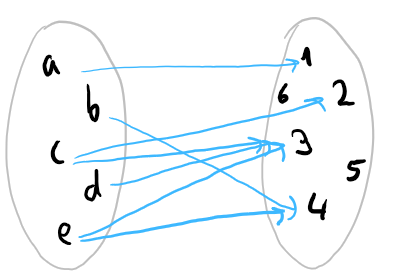
\includegraphics[width=.5\linewidth]{images/mengen_linkstotal.png}
	\end{center}
\end{frame}

\begin{frame}{Rechtstotalität}
	\begin{block}{Rechtstotale Relation}
		Eine Relation $R \subseteq A \times B$ heißt rechtstotal\pause , wenn für jedes $b \in B$ ein $a \in A$ existiert mit $(a,b) \in R$.
	\end{block}\pause
	
	Die rechte Seite der Relation ist also ``total'' aufgefüllt.\pause
	
	\markGreen{Wenn die Relation zusätzlich eine Abbildung ist, heißt diese dann} \markBlue{surjektiv}.\pause
	
	\begin{center}
		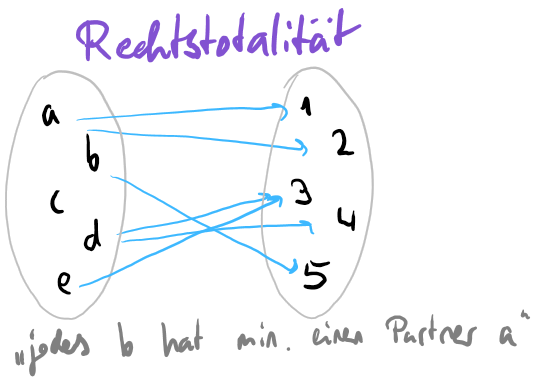
\includegraphics[width=.5\linewidth]{images/mengen_rechtstotal.png}
	\end{center}
\end{frame}

\begin{frame}{Linkseindeutigkeit}
	\begin{block}{Linkseindeutige Relation}
		Eine Relation $R \subseteq A \times B$ heißt linkseindeutig\pause , wenn für zwei beliebige Elemente $(a, \alpha) \in R, (b, \beta) \in R$ aus der Relation $R$ gilt: \pause wenn $a \neq b$, dann gilt auch $\alpha \neq \beta$. 
	\end{block}\pause
	
	Also: Keine zwei Elemente der linken Seite der Relation haben dasselbe rechte Element.\pause
	
	Angenommen, $a \neq b$ und $\alpha = \beta$. \pause $\Rightarrow$ offenbar nicht linkseindeutig.\pause
	
	\markGreen{Wenn die Relation zusätzlich eine Abbildung ist, heißt diese dann} \markBlue{injektiv}.\pause
	
	\begin{center}
		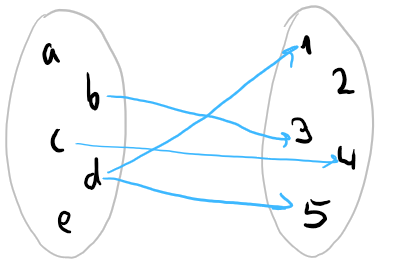
\includegraphics[width=.4\linewidth]{images/mengen_linkseindeutig.png}
	\end{center}
\end{frame}

\begin{frame}{Rechtseindeutig}
	\begin{block}{Rechtseindeutige Relation}
		Eine Relation $R \subseteq A \times B$ heißt rechtseindeutig\pause , wenn für zwei beliebige Elemente $(a, \alpha) \in R, (b, \beta) \in R$ aus der Relation $R$ gilt: \pause wenn $\alpha \neq \beta$, dann gilt auch $a \neq b$. 
	\end{block}\pause
	
	Also: Keine zwei Elemente der rechten Seite der Relation haben dasselbe linke Element.\pause
	
	\begin{center}
		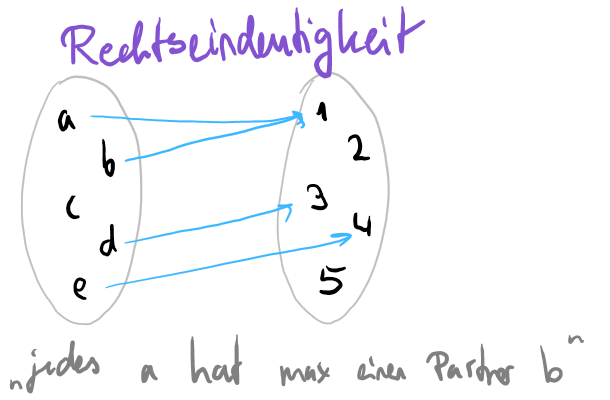
\includegraphics[width=.5\linewidth]{images/mengen_rechtseindeutig.png}
	\end{center}
\end{frame}

\ifdefined\printmode
\begin{frame}{Eigenschaften von Relationen}
	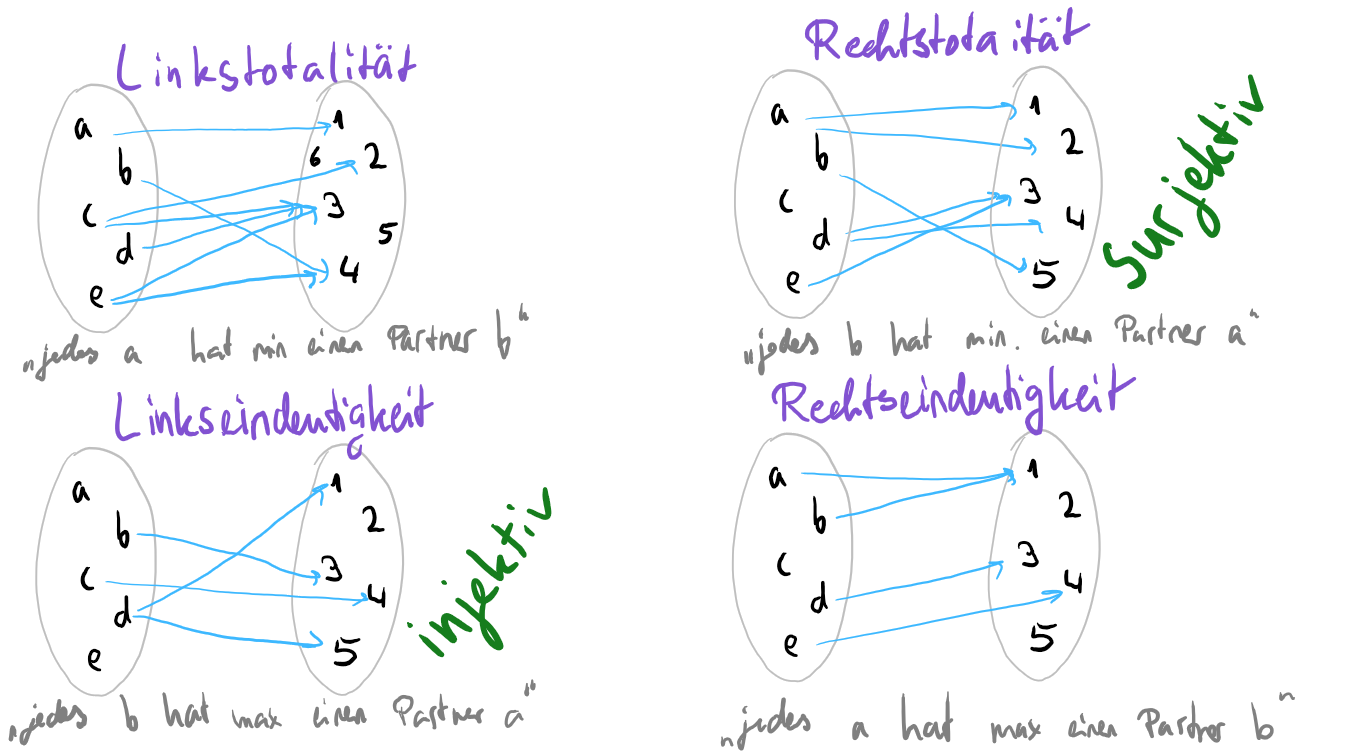
\includegraphics[width=\linewidth]{images/mengen_alle.png}
\end{frame}
\fi

\begin{frame}{Abbildung}
	\pause
	\begin{block}{Abbildung}
		Eine Relation $R$ heißt eine Abbildung, wenn sie linkstotal \emph{und} rechtseindeutig sind.
	\end{block}\pause
	
	\begin{itemize}
		\item Injektive Funktion: \pause \markGreen{linkstotal}, \markGreen{rechtseindeutig}, \markBlue{linkseindeutig}
		\pitem Surjektive Funktion: \pause \markGreen{linkstotal}, \markGreen{rechtseindeutig}, \markBlue{rechtstotal}
	\end{itemize}
	
	\pause
	
	\begin{block}{Bijektivität}
		Eine Relation heißt bijektiv, wenn sie injektiv und surjektiv ist.
	\end{block}
	
	\pause
	
	Damit ist sie \markGreen{linkstotal} und \markGreen{rechtseindeutig} (weil es eine Abbildung ist) und \markBlue{linkseindeutig} (injektiv) und \markBlue{rechtstotal} (surjektiv).
	
	\pause Tolle Eigenschaft: \pause Für jedes Element $(a, b) \in R$ der bijektiven Relation $R$ ist \emph{jedem} $a$ \emph{genau ein} $b$ zugeordnet. 
	
\end{frame}

\begin{frame}{Abbildungen Schreibweise}
	Seien $A = B = \R$, $f \subseteq A \times B$. \pause Wir suchen Relation, die für jedes $a \in A$ ein Element $(a, b) \in f$ enthält mit $b = a^2$.\pause
	
	$f = \{(0, 0), (0.1, 0.01), (2, 4), \dots\}$ 
	
	\pause Unendlich viele Elemente, und unmöglich alle zu nennen.
	
	\pause(Mathematischere) Schreibweise für Abbildungen:\pause
	
	$f : A \rightarrow B, a \mapsto a^2$\pause , also Quadratfunktion.
	
	\pause Ist diese Funktion injektiv oder surjektiv? \pause 
	
	\begin{itemize}
		\item Nicht injektiv, da z.B. $f(1) = f(-1)$\pause , also $(1, 1) \in f$ und $(-1, 1) \in f$.\pause
		\item Nicht surjektiv, da z.B. $-1$ nie als Funktionswert angenommen wird\pause , daher $(a, -1) \not\in f$ für beliebige $a \in A$.
	
	\end{itemize}
	
\end{frame}

%\ifdefined\fullcompile \else
\ifdefined\compileall
\else


\ifthenelse{\equal{\compiletype}{print}}
{

\begin{frame}{Informationen}
	
	\begin{columns}
		\begin{column}{0.5\textwidth}
			
			\begin{block}{Zum Tutorium}
				\begin{itemize}
					\item Lukas Bach
					\item Tutorienfolien auf: 
					\begin{itemize}
						\item \url{http://gbi.lukasbach.com}
					\end{itemize}
					\item Tutorium findet statt:
					\begin{itemize}
						\item Donnerstags, 14:00 - 15:30
						\item 50.34 Informatikbau, -107
					\end{itemize}
				\end{itemize}
			\end{block}
			
			\begin{block}{Mehr Material}
				\begin{itemize}
					\item Ehemalige GBI Webseite:
					\begin{itemize}
						\item \url{http://gbi.ira.uka.de}
						\item Altklausuren!
					\end{itemize}
				\end{itemize}
			\end{block}
			
		\end{column}
		\begin{column}{0.5\textwidth}
			
			\begin{block}{Zur Veranstaltung}
				\begin{itemize}
					\item Grundbegriffe der Informatik
					\item Klausurtermin:
					\begin{itemize}
						\item 06.03.2017, 11:00
						\item Zwei Stunden Bearbeitungszeit
						\item 6 ECTS für Informatiker und Informationswirte, 4 ECTS für Mathematiker und Physiker
					\end{itemize}
				\end{itemize}
			\end{block}
			
			\begin{block}{Zum Übungsschein}
				\begin{itemize}
					\item Übungsblatt jede Woche
					\item Ab 50\% insgesamt hat man den Übungsschein
					\item Keine Voraussetzung für die Klausur, aber für das Modul
				\end{itemize}
			\end{block}
			
		\end{column}
	\end{columns}
	
\end{frame}

}{}

\ifdefined\livebeamermode
	\begin{frame}
		
\includegraphics[width=\linewidth]{images/thatsall.png}
	\end{frame}
\fi

\end{document}

\fi
%\fi
\def\tutdate{4.11.2016}
\ifdefined\compileall \else
\ifdefined\compiletype
	\documentclass[handout]{beamer}
\else
	\documentclass{beamer}
	\def\compiletype{livebeamer}
\fi

\usepackage{templates/beamerthemekitwide}

\usepackage[utf8]{inputenc}
\usepackage[T1]{fontenc}
\usepackage[ngerman]{babel}
\usepackage{listings}
\usepackage{hyperref}
\usepackage{graphicx}

\usepackage{amsmath}
\usepackage{amsthm}
\usepackage{amssymb}
\usepackage{polynom}

\usepackage{ifthen}
\usepackage{adjustbox} % for \adjincludegraphics

\newcommand{\markBlue}[1]{\textcolor{kit-blue100}{#1}}
\newcommand{\markGreen}[1]{\textcolor{kit-green100}{#1}}

\newcommand{\pitem}{\pause\item}
\newcommand{\p}{\pause}

% -- MATH MACROS
\newcommand{\thistheoremname}{}
\newcommand{\G}{\mathbb{Z}}
\newcommand{\B}{\mathbb{B}}
\newcommand{\R}{\mathbb{R}}
\newcommand{\N}{\mathbb{N}}
\newcommand{\Q}{\mathbb{Q}}
\newcommand{\C}{\mathbb{C}}
\newcommand{\Z}{\mathbb{Z}}
\newcommand{\F}{\mathbb{F}}
\newcommand{\mi}{\mathrm{i}}
\renewcommand{\epsilon}{\varepsilon}


\newenvironment<>{taskblock}[1]{%
	\setbeamercolor{block title}{fg=kit-orange15,bg=kit-orange100}
	\setbeamercolor{block body}{fg=black,bg=kit-orange30}%
	\begin{block}#2{#1}}{\end{block}}

\setbeamertemplate{enumerate items}[default]

% Aussagenlogik Symbole
\newcommand{\W}{w}
\renewcommand{\F}{f}

% Kodierung
\newcommand{\frepr}{\textbf{repr}}
\newcommand{\fRepr}{\textbf{Repr}}
\newcommand{\fZkpl}{\textbf{Zkpl}}
\newcommand{\fbin}{\textbf{bin}}
\newcommand{\fdiv}{\textbf{ div }}
\newcommand{\fmod}{\textbf{ mod }}

\title[Grundbegriffe der Informatik]{Grundbegriffe der Informatik\\Tutorium 33}
\subtitle{}
\author{Lukas Bach, lukas.bach@student.kit.edu}
\date{\tutdate}

\institute{}

\titlelogo{lukasbach}

\titleimage{bg}
%\titleimage{bg-advent}


\ifthenelse{\equal{\compiletype}{livebeamer}}
	{
		\def\livebeamermode{1}
	}{}

\ifthenelse{\equal{\compiletype}{print}}
	{
		\def\printmode{1}
	}{}

\setbeamercovered{invisible}

%\usepackage[citestyle=authoryear,bibstyle=numeric,hyperref,backend=biber]{biblatex}
%\addbibresource{templates/example.bib}
%\bibhang1em

\begin{document}
	
\selectlanguage{ngerman}


%title page
\begin{frame}
	\titlepage
\end{frame}

%table of contents
\ifdefined\printmode
	\ifdefined\compileall \else
	\begin{frame}{Gliederung}
		\tableofcontents
	\end{frame}
\fi\fi

\fi

\section{Wiederholung}
\begin{frame}{Wiederholung}
	\pause
	
	$A := \{a, b, c\}, B := \{b, c, d\}, C := \{a, d\}$
	
	\begin{itemize}
		\pitem $A \cap B$ \pause $= \{b, c\}$
		\pitem $A \cup B$ \pause $= \{a, b, c, d\}$
		\pitem $A \backslash B$ \pause $= \{a\}$
		\pitem $C^2$ \pause $ = C \times C$ \pause $= \{(a, a), (a, d), (d, a), (d, d)\}$
		\pitem $2^C$ \pause $ = \{\emptyset$ \pause $, \{a, d\}$, \pause $\{a\}$, \pause $\{d\}\}$
		\pitem Unterschied zwischen $\{a, b\}$ und $(a, b)$?
		\pitem Definition von...
		\begin{itemize}
			\pitem Alphabet?
			\pitem Abbildung?
		\end{itemize}
	\end{itemize}
\end{frame}

\section{Wörter}

\begin{frame}{Wörter}
	\pause
	\begin{block}{Konkatenation}
		Durch Konkatenation werden einzelne Buchstaben aus einem Alphabet miteinander verbunden.
	\end{block}

	\begin{itemize}
		\pitem Symbol: $\cdot$\pause , also zwei Buchstaben $a$ und $b$ miteinander konkateniert: $a \cdot b$.
		\pitem Nicht kommutativ\pause : $a \cdot b \neq b \cdot a$
		\pitem Aber assoziativ\pause : $(a \cdot b) \cdot c = a \cdot (b \cdot c)$
		\pitem Kurzschreibweise\pause : Ohne Punkte\pause , also $a \cdot b = ab$
	\end{itemize}
\end{frame}

\begin{frame}{Wörter}
	\pause
	\begin{block}{Wörter: Intuitivere Definition}
		Ein Wort $w$ \pause entsteht durch die Konkatenation durch Buchstaben aus einem Alphabet.
	\end{block}

	\pause Also Abfolge von Zeichen.

	\pause Sei $A := \{a, b, c\}$.

	\begin{itemize}
		\pitem Mögliche Worte: \pause $w_1 := a \cdot b$\pause , $w_2 = b \cdot c \cdot c$\pause , $w_3 = a \cdot c \cdot c \cdot b \cdot a$.
		\pitem Keine möglichen Worte: \pause $d$.
		\pitem Konkatenation nicht kommutativ\pause : Wort $abc$ \pause ist ungleich dem Wort $bca$.
	\end{itemize}
\end{frame}

\begin{frame}{Wörter}
	\pause
	\begin{block}{Wörter: Abstraktere Definition}
		Ein Wort $w$ \pause über dem Alphabet $A$ \pause ist definiert als surjektive Abbildung \pause $w : \Z_n \rightarrow A$. \pause Dabei heißt $n$ \pause die Länge $|w|$ des Wortes.
	\end{block}

	\begin{itemize}
		\pitem $\Z_n$ \pause $ = \{i \in \N : \pause 0 \leq i < n \}$
		
		\pause $\Z_3 \pause = \{0, 1, 2\}, \pause \Z_2 = \{0, 1\}, \Z_0 = \emptyset$.
		
		\pitem Länge oder Kardinalität eines Wortes: \pause $|w|$. \pause $|abcde|$ \pause $= 5$.
		
		\pitem Wort $w = abdec$ als Relation aufgeschrieben: \pause $w = \{(0, a), (1, b), (2, d), (3, e), (4, c)\}$. \pause Also $w(0) = a, w(1) = b, w(2) = d, \dots$
		
		\pause Damit sieht man auch: $|w| = |\{(0, a), (1, b), (2, d), (3, e), (4, c)\}| = 5$.
	\end{itemize}
\end{frame}

\begin{frame}{Wörter}
	\pause
	\begin{itemize}
		\item Wort der Kardinalität 0?
	\end{itemize}

	\pause

	\begin{block}{Das leere Wort}
		Das leere Wort \pause $\varepsilon$ \pause ist definiert ein Wort mit Kardinalität 0\pause , also mit 0 Zeichen.
	\end{block}

	\begin{itemize}
		\pitem Leere Wort wird interpretiert als ``nicht sichtbar'' und kann überall platziert werden\pause : $aabc \pause = a\epsilon abc = \epsilon\epsilon a\epsilon bc \epsilon$.
		\pitem $|\{\epsilon\}|$ \pause $ = 1$\pause , die Menge ist nicht leer! \pause Das leere Wort ist nicht \emph{nichts}! \pause (Vergleiche leere Menge)
		\pitem $|\epsilon| = 0$.
	\end{itemize}
\end{frame}

\begin{frame}{Mehr über Wörter}

	\pause
	
	\begin{block}{$A^n$}
		Zu einem Alphabet $A$ \pause ist $A^n$ definiert als die Menge aller Wörter \pause der Länge $n$ \pause über dem Alphabet $A$.
	\end{block}

	\begin{itemize}
		\pitem Nicht mit Mengenpotenz verwechseln!
		\pitem $A := \{a, b, c\}$\pause , $A^2 = \pause \{aa, ab, ac, ba, bb, bc, ca, cb, cc\}$. \pause $A^1 \pause = A, \pause A^0 = \{\epsilon\}$.
	\end{itemize}
	
	\pause Die Menge aller Wörter \pause \emph{beliebiger} Länge: \pause
	\begin{itemize}
		\item $A^* := \bigcup_{i \in \N_0} A_i$
		\pitem $A := \{a, b, c\}$\pause . $aa \in A^*\pause , abcabcabc \in A^*\pause , aaaa \in A^*\pause , \epsilon \in A^*$.
	\end{itemize}
\end{frame}

\begin{frame}{Mehr über Wörter}
	
	\pause
	
	Konkatenation von Wörtern:
	
	\begin{itemize}
		\pitem $lager \cdot regal$ \pause $ = lagerregal$
		\pitem $lag \cdot erregal = lagerregal$
	\end{itemize}
	
	\pause
	
	\begin{block}{Konkatenation von Wörtern.}
		\begin{align*}
		w_1\cdot w_2 : \Z_{m+n} &\rightarrow A_1\cup A_2 \\
		i & \mapsto \begin{cases}
		w_1(i) & \text{ falls } 0\leq i<m \\
		w_2(i-m) & \text{ falls } m \leq i<m+n
		\end{cases}
		\end{align*}
	\end{block}

	\pause
	
	\begin{itemize}
		\item Warum $\Z_{m+n}$? \pause Wörter $w_1$ und $w_2$ \pause mit $|w_1| = m$ und $|w_2| = n$ werden konkateniert\pause , also neues Wort hat Länge $m + n$.
	\end{itemize}

\end{frame}

\begin{frame}{Mehr über Wörter}
	
	\begin{block}{Konkatenation von Wörtern.}
		\begin{align*}
		w_1\cdot w_2 : \Z_{m+n} &\rightarrow A_1\cup A_2 \\
		i & \mapsto \begin{cases}
		w_1(i) & \text{ falls } 0\leq i<m \\
		w_2(i-m) & \text{ falls } m \leq i<m+n
		\end{cases}
		\end{align*}
	\end{block}

	\pause
	
	\begin{center}
	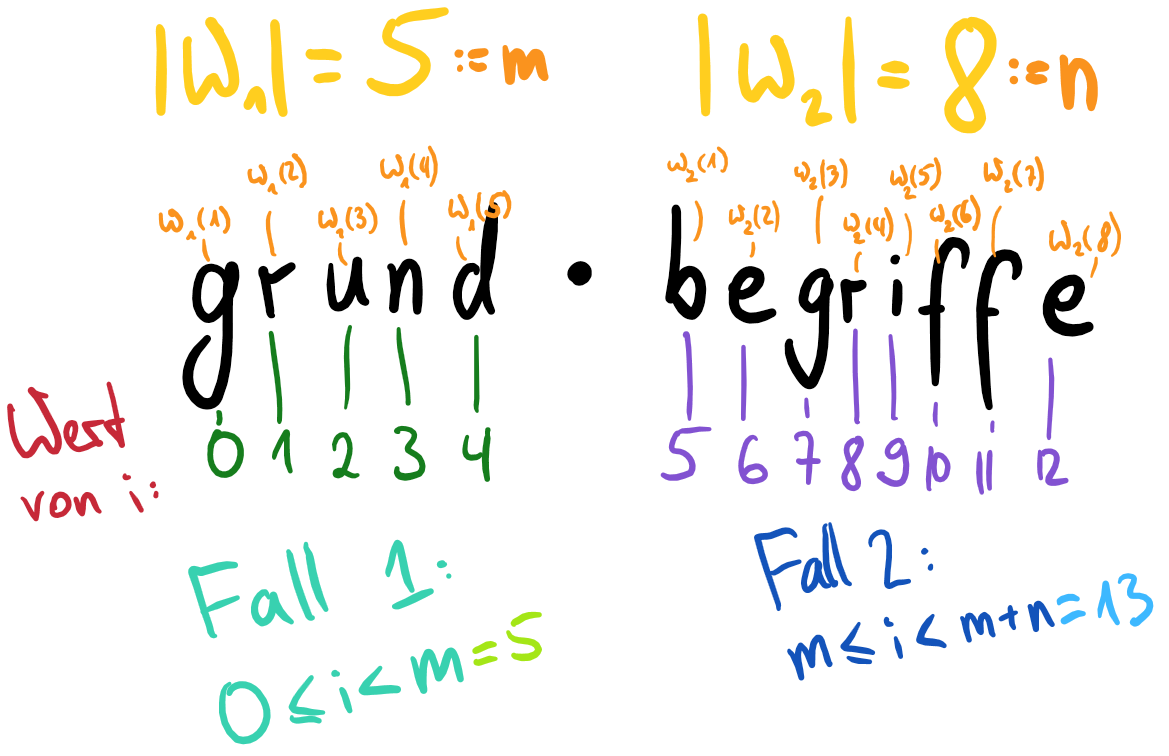
\includegraphics[width=.6\linewidth]{images/wortkonkatenation.png}
	\end{center}

\end{frame}

\begin{frame}{Mehr über Wörter}
	\begin{itemize}
		\pitem Immernoch: \pause Reihenfolge ist wichtig! \pause $OTT \cdot O = OTTO \pause \neq OOTT = O \cdot OTT$
		\pitem Auf wieviele Weisen kann man $abc$ als Konkatenation nichtleerer Wörter schreiben? \pause $abc$\pause , $a \cdot bc$\pause , $ab \cdot c$\pause , $a \cdot b \cdot c$. 
		\pitem Wortkonkatenation mit dem leeren Wort\pause : $w \cdot \epsilon$ \pause $ = w$ \pause $ = \epsilon \cdot w$.
	\end{itemize}
\end{frame}

\begin{frame}{Mehr über Wörter}
	\pause
	
	\begin{block}{Wort Potenzen}
		Sich direkt wiederholende Teilworte kann man als Wortpotenz darstellen\pause , daher $w_i^n = w_i \cdot w_i \cdots w_i$ (n $\times$ mal).
	\end{block}

	\begin{itemize}
		\pitem $a^4 = aaaa$\pause , $b^3 = bbb$\pause , $c^0 = \pause \epsilon$\pause , $d^1 = \pause d$.
		\pitem $a^3c^2b^6 \pause = aaaccbbbbbb$.
		\pitem $b \cdot a \cdot (n \cdot a)^2$ \pause $ = banana$.
		\pitem $(a^3b^2)^2c(a^2bcb^3)^3dd$ \pause $=(aaabb)^2c(aabcbbb)^3dd$ \pause $ = aaabb \cdot aaabb \cdot \quad c \quad \cdot aabcbbb \cdot aabcbbb \cdot aabcbbb \cdot \quad dd$.
	\end{itemize}
\end{frame}

\begin{frame}{Übung zu Wörter}
	Sei $A$ ein Alphabet.
	
	\begin{taskblock}{Übung zu Wörter}
		\begin{enumerate}
			\item Finde Abbildung $f: A^* \rightarrow A^*$, sodass für alle $w \in A^*$ gilt: \\\quad $2 \cdot |w| = |f(w)|$.
			\item Finde Abbildung $g: A^* \rightarrow A^*$, sodass für alle $w \in A^*$ gilt: \\\quad $|w| + 1 = |g(w)|$.
			\item Finde Abbildung $h: A^* \rightarrow A^*$, sodass für alle $w \in A^*$ gilt: \\\quad $\lfloor \frac{|w|}{2}\rfloor = |h(w)|$. (Zusatz)
			\item Sind $f, g, h$ injektiv und/oder surjektiv?
		\end{enumerate}
	\end{taskblock}

	\pause
	
	\begin{enumerate}
		\item $f: A^* \rightarrow A^*, w \mapsto w \cdot w$.
		\pitem $g: A^* \rightarrow A^*, w \mapsto w \cdot x, x \in A$.
		\pitem $h: A^* \rightarrow A^*, w \mapsto \hat{w}$ mit $ \hat{w}_i = 
			\left\{
			\begin{array}{ll}
			w_i  & \mbox{wenn } i \leq \lfloor\frac{|w|}{2}\rfloor \\
			\epsilon & \mbox{sonst }
			\end{array}
			\right\}
		$ und $i \in \Z_{|w|}$.
	\end{enumerate}
\end{frame}

\begin{frame}{Übung zu Wörter}
	\begin{enumerate}
		\item $f: A^* \rightarrow A^*, w \mapsto w \cdot w$.
		\begin{itemize}
			\pitem $f$ ist injektiv\pause , denn jedes $w$ aus der Bildmenge wird von maximal einem Wort abgebildet.
			\pitem $f$ ist nicht surjektiv\pause , denn z.B. bildet nichts auf $x \in A$ ab (oder auf andere Wörter mit ungerader Anzahl an Buchstaben).
		\end{itemize}
		\pitem $g: A^* \rightarrow A^*, w \mapsto w \cdot x, x \in A$.
		\begin{itemize}
			\pitem $g$ ist injektiv.
			\pitem $g$ ist nicht surjektiv\pause , denn z.B. bildet nichts auf $\epsilon$ ab.
		\end{itemize}
		\pitem $h: A^* \rightarrow A^*, w \mapsto \hat{w}$ mit $ \hat{w}_i = 
		\left\{
		\begin{array}{ll}
		w_i  & \mbox{wenn } i \leq \lfloor\frac{|w|}{2}\rfloor \\
		\epsilon & \mbox{sonst }
		\end{array}
		\right\}
		$ und $i \in \Z_{|w|}$.
		\begin{itemize}
			\pitem $h$ ist nicht injektiv\pause , denn z.B. $x = h(xy) = h(xz)$ mit $x,y,z \in A$.
			\pitem $h$ ist surjektiv\pause , denn für jedes $w \in A^*$ existiert ein $\hat{w} \in A^*$ mit $\hat{w} = w \cdot w$ sodass $h(\hat{w}) = w$.
		\end{itemize}
	\end{enumerate}
\end{frame}

\section{Formale Sprachen}

\begin{frame}{Formale Sprache}
	\begin{itemize}
		\pitem Was war nochmal $A^*$? Menge aller Wörter \emph{beliebiger} Länge über Alphabet $A$.
	\end{itemize}

	\pause
	
	\begin{block}{Formale Sprache}
		Eine Formale Sprache $L$ \pause über einem Alphabet $A$ ist eine Teilmenge $L \subseteq A^*$.
	\end{block}

	\begin{itemize}
		\pitem Zufälliges Beispiel: \pause $A := \{b, n, a\}$.
		\begin{itemize}
			\pitem $L_1 := \{ban, baan, nba, aa\}$ ist eine mögliche formale Sprache über $A$.
			\pitem $L_2 := \{banana, bananana, banananana, ...\}$ \pause $ = \{w : w = bana(na)^k, k \in \N\}$ auch.
			\pitem $L_3 := \{ban, baan, baaan, ...\}$ auch. \pause Andere Schreibweise? \pause \\ $ L_3 = \{w : w = ba^kn, k \in \N \}$
		\end{itemize}
		\pitem Formale Sprachen sind also nicht zwangsweise endliche Mengen.
		\pitem Praktischeres Beispiel: $A := \{w : w $ ist ein ASCII Symbol $\}$.
		\begin{itemize}
			\pitem $L_4 := \{class, if, else, while, for, ...\}$ ist eine formale Sprache über $A$.
			\pitem $L_5 := \{w : w = a \cdot b$ mit $a$ als Großbuchstabe und $b$ als Groß- oder Kleinbuchstabe $ \} \pause \backslash L_4$ \pause ist eine formale Sprache von korrekten Klassennamen in Java.
		\end{itemize}
	\end{itemize}
\end{frame}

\begin{frame}{Übung zu formalen Sprachen}
	\pause
	
	$A := \{a, b\}$
	
	\begin{itemize}
		\pitem Sprache $L$ aller Wörter über $A$, die nicht das Teilwort $ab$ enthalten?
		\begin{itemize}
			\pitem Was passiert wenn ein solches Wort ein $a$ enthält? \pause Dann keine $b$'s mehr!
			\pitem $L = \{w_1 \cdot w_2 : w_1 \in \{b\}^*$ und $w_2 \in \{a\}^* \}$
			\pitem Andere Möglichkeit\pause : Suche Wörter mit $ab$ und nehme diese Weg.
			\pitem $L = \{a, b\}^*\pause \backslash\{ w_1 \cdot ab \cdot w_2 : w_1, w_2 \in \{a,b\}^* \}$
		\end{itemize}
	\end{itemize}
\end{frame}

\begin{frame}{Übung zu formalen Sprachen}
	
	Sei $A := \{a, b\}, B := \{0, 1\}$.
	
	\begin{taskblock}{Aufgabe zu formalen Sprachen}
		\begin{enumerate}
			\item Sprache $L_1 \subseteq A^*$ von Wörtern, die mindestens drei $b$'s enthalten.
			\item Sprache $L_2 \subseteq A^*$ von Wörtern, die gerade Zahl von $a$'s enthält.
			\item Sprache $L_3 \subseteq B^*$ von Wörtern, die, interpretiert als Binärzahl eine gerade Zahl sind.
		\end{enumerate}
	\end{taskblock}

	\pause
	
	\begin{enumerate}
		\item $L_1 \pause = \{w = w_1  b  w_2  b  w_3 b w_4 : w_1,w_2,w_3,w_4 \in A^* \}$
		\pitem $L_2 \pause = \{w = (w_1 a w_2 a w_3)^* : w_1,w_2,w_3 \in \{b\}^* \}$ \pause (Ist da $\epsilon$ drin?)
		\pitem $L_3 \pause = \{w = w \cdot 0 : w \in B^* \}$
	\end{enumerate}
\end{frame}

\ifdefined\compileall
\else


\ifthenelse{\equal{\compiletype}{print}}
{

\begin{frame}{Informationen}
	
	\begin{columns}
		\begin{column}{0.5\textwidth}
			
			\begin{block}{Zum Tutorium}
				\begin{itemize}
					\item Lukas Bach
					\item Tutorienfolien auf: 
					\begin{itemize}
						\item \url{http://gbi.lukasbach.com}
					\end{itemize}
					\item Tutorium findet statt:
					\begin{itemize}
						\item Donnerstags, 14:00 - 15:30
						\item 50.34 Informatikbau, -107
					\end{itemize}
				\end{itemize}
			\end{block}
			
			\begin{block}{Mehr Material}
				\begin{itemize}
					\item Ehemalige GBI Webseite:
					\begin{itemize}
						\item \url{http://gbi.ira.uka.de}
						\item Altklausuren!
					\end{itemize}
				\end{itemize}
			\end{block}
			
		\end{column}
		\begin{column}{0.5\textwidth}
			
			\begin{block}{Zur Veranstaltung}
				\begin{itemize}
					\item Grundbegriffe der Informatik
					\item Klausurtermin:
					\begin{itemize}
						\item 06.03.2017, 11:00
						\item Zwei Stunden Bearbeitungszeit
						\item 6 ECTS für Informatiker und Informationswirte, 4 ECTS für Mathematiker und Physiker
					\end{itemize}
				\end{itemize}
			\end{block}
			
			\begin{block}{Zum Übungsschein}
				\begin{itemize}
					\item Übungsblatt jede Woche
					\item Ab 50\% insgesamt hat man den Übungsschein
					\item Keine Voraussetzung für die Klausur, aber für das Modul
				\end{itemize}
			\end{block}
			
		\end{column}
	\end{columns}
	
\end{frame}

}{}

\ifdefined\livebeamermode
	\begin{frame}
		
\includegraphics[width=\linewidth]{images/thatsall.png}
	\end{frame}
\fi

\end{document}

\fi
\def\tutdate{11.11.2016}
\ifdefined\compileall \else
\ifdefined\compiletype
	\documentclass[handout]{beamer}
\else
	\documentclass{beamer}
	\def\compiletype{livebeamer}
\fi

\usepackage{templates/beamerthemekitwide}

\usepackage[utf8]{inputenc}
\usepackage[T1]{fontenc}
\usepackage[ngerman]{babel}
\usepackage{listings}
\usepackage{hyperref}
\usepackage{graphicx}

\usepackage{amsmath}
\usepackage{amsthm}
\usepackage{amssymb}
\usepackage{polynom}

\usepackage{ifthen}
\usepackage{adjustbox} % for \adjincludegraphics

\newcommand{\markBlue}[1]{\textcolor{kit-blue100}{#1}}
\newcommand{\markGreen}[1]{\textcolor{kit-green100}{#1}}

\newcommand{\pitem}{\pause\item}
\newcommand{\p}{\pause}

% -- MATH MACROS
\newcommand{\thistheoremname}{}
\newcommand{\G}{\mathbb{Z}}
\newcommand{\B}{\mathbb{B}}
\newcommand{\R}{\mathbb{R}}
\newcommand{\N}{\mathbb{N}}
\newcommand{\Q}{\mathbb{Q}}
\newcommand{\C}{\mathbb{C}}
\newcommand{\Z}{\mathbb{Z}}
\newcommand{\F}{\mathbb{F}}
\newcommand{\mi}{\mathrm{i}}
\renewcommand{\epsilon}{\varepsilon}


\newenvironment<>{taskblock}[1]{%
	\setbeamercolor{block title}{fg=kit-orange15,bg=kit-orange100}
	\setbeamercolor{block body}{fg=black,bg=kit-orange30}%
	\begin{block}#2{#1}}{\end{block}}

\setbeamertemplate{enumerate items}[default]

% Aussagenlogik Symbole
\newcommand{\W}{w}
\renewcommand{\F}{f}

% Kodierung
\newcommand{\frepr}{\textbf{repr}}
\newcommand{\fRepr}{\textbf{Repr}}
\newcommand{\fZkpl}{\textbf{Zkpl}}
\newcommand{\fbin}{\textbf{bin}}
\newcommand{\fdiv}{\textbf{ div }}
\newcommand{\fmod}{\textbf{ mod }}

\title[Grundbegriffe der Informatik]{Grundbegriffe der Informatik\\Tutorium 33}
\subtitle{}
\author{Lukas Bach, lukas.bach@student.kit.edu}
\date{\tutdate}

\institute{}

\titlelogo{lukasbach}

\titleimage{bg}
%\titleimage{bg-advent}


\ifthenelse{\equal{\compiletype}{livebeamer}}
	{
		\def\livebeamermode{1}
	}{}

\ifthenelse{\equal{\compiletype}{print}}
	{
		\def\printmode{1}
	}{}

\setbeamercovered{invisible}

%\usepackage[citestyle=authoryear,bibstyle=numeric,hyperref,backend=biber]{biblatex}
%\addbibresource{templates/example.bib}
%\bibhang1em

\begin{document}
	
\selectlanguage{ngerman}


%title page
\begin{frame}
	\titlepage
\end{frame}

%table of contents
\ifdefined\printmode
	\ifdefined\compileall \else
	\begin{frame}{Gliederung}
		\tableofcontents
	\end{frame}
\fi\fi

\fi


\section{Aussagenlogik}

\begin{frame}{Aussagenlogik}
	\begin{itemize}
		\pitem Das wars erst mal zu formalen Sprachen.
		\pitem Heute ist Freitag.
		\pitem Die Menge aller Männer dieser Welt ist disjunkt zur Menge aller Frauen dieser Welt.
	\end{itemize}

	\pause
	
	Das sind alles Aussagen. \pause Aussagen sind entweder \emph{wahr} \pause oder \emph{falsch}.
\end{frame}

\begin{frame}{Aussagenlogik}
	\pause 
	
	Wir kapseln Aussagen und verwendet Variablen dafür. \pause 
	
	Zum Beispiel:
	
	\begin{itemize}
		\pitem $A := $ ``Die Straße ist nass.''
		\pitem $B := $ ``Es regnet.''
	\end{itemize}

	\pause Aussagen lassen sich verknüpfen:
	
	\begin{itemize}
		\pitem \markGreen{Logisches Und:} \pause $A \land B \pause = A$ und $B \pause = $ Die Straße ist nass und es regnet.
		\pitem \markGreen{Logisches Oder:} \pause $A \lor B \pause = A$ oder $B \pause = $ Die Straße ist nass oder es regnet\pause . Es kann auch beides wahr sein.
		\pitem \markGreen{Negierung:} \pause $\lnot A \pause = $ nicht $A \pause = $ Die Straße ist nicht nass.
		\pitem \markGreen{Implikation:} \pause $A \rightarrow B \pause = $ Aus $A$ folgt $B \pause = $ Wenn die Straße nass ist, dann regnet es.
		\pitem \markGreen{Äquivalenz:} \pause $A \leftrightarrow B \pause = A$ und $B$ sind äquivalent $\pause = $ Die Straße ist \emph{genau dann} nass, \emph{wenn} es regnet.
		\begin{itemize}
			\pitem $A \leftrightarrow B = (A \rightarrow B) \land (B \rightarrow A)$\pause , also die Straße ist nass wenn es regnet \emph{und} es regnet wenn die Straße nass ist.
		\end{itemize}
	\end{itemize}

\end{frame}

\begin{frame}{Übung zu Aussagenlogik}
	
	\begin{itemize}
		\item $A := $ ``Die Straße ist nass.''
		\item $B := $ ``Es regnet.''
		\item $C := $ ``$\pi$ ist gleich $3$.''
	\end{itemize}

	\begin{itemize}
		\pitem Was ist $B \rightarrow C$? \pause ``Wenn es regnet, ist $\pi$ gleich $3$.''
	\end{itemize}

	\pause
	
	% Aus Skriptum, Kapitel 5.3 Boolesche Funktionen
	\begin{center}
		\begin{tabular}{c|c||c|c|c|c}%*{2}{>{$}c<{$}}|*{4}{>{$}c<{$}}
			\hline
			$x_1$ & $x_2$ & $\lnot x_1$ & $x_1 \land x_2$ & $x_1 \lor x_2$ & $x_1 \rightarrow x_2$ \\
			\hline
			\F & \F & \W & \F & \F & \W \\
			\F & \W & \W & \F & \W & \W \\
			\W & \F & \F & \F & \W & \F \\
			\W & \W & \F & \W & \W & \W \\
			\hline
		\end{tabular}
	\end{center}
	
\end{frame}

\begin{frame}{Syntax der Aussagenlogik}
	\pause
	Menge der Aussagevariablen:
	
	\pause\quad $Var_{AL} \pause \subseteq \{P_i : i \in \N_0\}$ \pause oder $\{P, Q, R, S, \dots\}$
	
	\pause Alphabet der Aussagenlogik:
	
	\pause\quad $A_{AL} = \{(, ), \lnot, \land, \lor, \rightarrow, \leftrightarrow\} \cup Var_{AL}$
\end{frame}

\begin{frame}{Boolesche Funktionen}
\begin{block}{Boolesche Funktionen}
	Eine boolsche Funktion ist eine Abbildung \pause der Form $f: \B^n \rightarrow \B$ \pause mit $\B = \{w, f\}$.
\end{block}

Typische Boolsche Funktionen\pause : $b_\lnot (x) \pause = \lnot x$\pause , $b_\lor (x_1, x_2) \pause = x_1 \lor x_2$ \dots
\end{frame}

\begin{frame}{Interpretationen}
	\begin{block}{Interpretation}
		\pause Eine Interpretation ist eine Abbildung $I : V \rightarrow \B$\pause , die einer Variablenmenge eine ``Interpretation''\pause , also wahr oder falsch zuordnet.
	\end{block}

\pause Weiter legt man $val_I(F)$ als Auswertung einer aussagenlogischer Formel $F$ fest.
\pause
	\newcommand{\val}{val}
	\begin{align*}
	\val_I(X)         &= I(X) \\
	\val_I(\lnot G)   &= b_{\lnot}(\val_I(G)) \\
	\val_I(G \land H) &= b_{\land}(\val_I(G), \val_I(H)) \\
	\val_I(G \lor H)  &= b_{\lor}(\val_I(G)  \val_I(H)) \\
	\val_I(G \rightarrow H)&= b_{\rightarrow}(\val_I(G), \val_I(H))
	\end{align*}
\end{frame}

\begin{frame}{Übung zu Interpretationen}
	
	
	\begin{itemize}
		\item Wie viele Interpretationen gibt es bei k = 1, 2, 3 Variablen?
		\item Wie viele Interpretationen gibt es bei k+1 Variablen im Vergleich zu k Variablen?
	\end{itemize}
	
\end{frame}	

\begin{frame}{Übung zur Aussagenlogik}
	\pause Sei $A := \W, B := \W, C := \F$.
	
	\begin{itemize}
		\pitem Ist $(A \land B) \lor \lnot C$ wahr oder falsch? \pause $(A \land B) \lor \lnot C \pause = (\W \land \W) \lor \lnot \F \pause = \W \lor \lnot \F = \pause \W \lor \W \pause = \W$\pause , die Aussage ist also wahr.
		\pitem Ist $\lnot (A \lor A)$ wahr oder falsch? \pause Falsch! \pause Wann ist $\lnot (A \lor A)$ im allgemeinen wahr? \pause Genau dann, wenn $\lnot A$ wahr ist.
	\end{itemize}

	\pause

	\begin{block}{Aussagen Äquivalenz}
		Erinnerung: \pause $A \leftrightarrow B$ heißt: \pause $A \rightarrow B \land B \rightarrow A$. 
		
		\pause Wenn zwei Aussagen äquivalent sind, sind ihre Wahrheitswerte immer gleich\pause , wenn die Wahrheitswerte, von denen sie abhängen, gleich sind. 
		
		\pause Mann sagt und schreibt dann: \pause $A$ ist \emph{genau dann} wahr, \emph{wenn} $B$ wahr ist.
	\end{block}

	\begin{itemize}
		\pitem $\lnot (A \lor A)$ ist genau dann wahr\pause , wenn $\lnot A$ wahr ist\pause , also gilt:  $\lnot (A \lor A) \pause \leftrightarrow \lnot A$. 
	\end{itemize}
\end{frame}

\begin{frame}{Mehr zu Äquivalenz}
\pause
	\begin{block}{Alternative Definition zu Äquivalenz}
		Zwei Formeln G und H heißen äquivalent, wenn für jede Interpretation gilt $val_I(G) = val_I(H)$.
	\end{block}\pause

	Vorher Äquivalenz von Formeln unter gegebener Interpretation\pause , diesmal Äquivalenz von Formeln unter beliebiger Interpretation.\pause

	\textbf{Bemerkung}\\
	\begin{itemize}
		\pitem Man schreibt $G \equiv  H$
		\pitem $\mathbb{B}^V \rightarrow \mathbb{B}: I \mapsto val_I(G)$
	\end{itemize}\pause
	\textbf{Beispiele}\\\pause
	$(\lnot(\lnot P))$ ist äquivalent zu $P$\\\pause
	$(\lnot(P\land Q))$ ist äquivalent zu $((\lnot P) \lor (\lnot Q))$
\end{frame}

\begin{frame}{Beispiele zu Äquivalenz}
	\begin{itemize}
		\pitem Ein Wort $w$ hat die Länge $n$ $\leftrightarrow |w| = n$.
		\pitem Die Vereinigung zweier Mengen $A$ und $B$ hat die Kardinalität $|A| + |B|$ \pause $\leftrightarrow$ $A \cap B = \emptyset$ \pause $\leftrightarrow$ $A$ und $B$ sind disjunkt.
		\pitem $p$ ist eine rationale Zahl \pause $\leftrightarrow$ $p$ lässt sich darstellen als $p = \frac{a}{b}, a\in \Z, b \in \N$ \pause $\leftrightarrow$ $p \in \Q$.
	\end{itemize}	
\end{frame}

\begin{frame}{Wahrheitstabellen}
	\begin{itemize}
		\item $(((P \rightarrow Q) \lor Q) \rightarrow (P \land \lnot Q))$
	\end{itemize}

	\begin{center}
		\begin{tabular}{c|c||c|c|c|c}%*{2}{>{$}c<{$}}|*{4}{>{$}c<{$}}
			\hline
				$P$ & $Q$ & $(P \land Q)$ & $\lor Q$ & $\rightarrow$ & $(P \land \lnot Q)$ \\\hline
				
				\visible<1->{\W} & \visible<1->{\W} & \visible<2->{\W} & \visible<6->{\W} & \visible<14->{\F} & \visible<10->{\F} \\\hline
				
				\visible<1->{\W} & \visible<1->{\F} & \visible<3->{\F} & \visible<7->{\F} & \visible<15->{\W} & \visible<11->{\W} \\\hline
				
				\visible<1->{\F} & \visible<1->{\W} & \visible<4->{\F} & \visible<8->{\W} & \visible<16->{\F} & \visible<12->{\F} \\\hline
				
				\visible<1->{\F} & \visible<1->{\F} & \visible<5->{\F} & \visible<9->{\F} & \visible<17->{\W} & \visible<13->{\F} \\\hline
				
		\end{tabular}
	\end{center}
\end{frame}

\begin{frame}{Übungen zu Aussagenlogik}
	\begin{taskblock}{Übungen zu Aussagenlogik}
		\begin{itemize}
			\item Schreibe Wahrheitstabellen zu den Formeln um den Wahrheitsgehalt festzustellen.
				\item $\lnot(P \land Q) \land \lnot (Q \land P)$
				\item $(P \land Q \land R) \leftrightarrow (\lnot P \lor Q)$
				\item $(A\land(B\lor C))\leftrightarrow ((A\land B)\lor(A\land C))$
			\item Welche dieser Aussagen sind wahr?
				\item $\lnot (P \land Q) = \lnot P \lor \lnot Q$
				\item $P \land P = P \lor P$
				\item $(P \lor Q) \land R = (P \land R) \lor (Q \land R)$
		\end{itemize}
	\end{taskblock}
\end{frame}

\begin{frame} {Wahrheitstabellen}
	\begin{center}
		\begin{tabular}{|c|c|c|c|c|c|c|}
			\hline
			$A$&$B$& $\lnot A$& $A \land B$ & $A\lor B$ &$A\rightarrow B$ &$A \leftrightarrow B$\\
			\hline
			w&w&f&w&w&w&w\\
			w&f&f&f&w&f&f\\
			f&w&w&f&w&w&f\\
			f&f&w&f&f&w&w\\
			\hline
		\end{tabular}
	\end{center}

	\begin{taskblock}{Aufgabe}
		Finde einen logischen Ausdruck in A und B unter Verwendung von $\land, \lor$ und $\lnot$, der die Aussage ``Entweder A oder B'' repräsentiert	
	\end{taskblock}
\end{frame}

\begin{frame}{Wahrheitstabellen}
	
	\begin{taskblock}{Aufgabe}
		Finde einen logischen Ausdruck in A und B unter Verwendung von $\land, \lor$ und $\lnot$, der die Aussage ``Entweder A oder B'' repräsentiert	
	\end{taskblock}

	\textbf{Lösung}
	\begin{center}
		\begin{tabular}{|c|c|c|c|c|}
			\hline
			$A$&$B$& $A \land \lnot B$& $\lnot A \land B$ & $(A \land \lnot B) \lor (\lnot A \land B) $\\
			\hline
			w&w&f&f&f\\
			w&f&w&f&w\\
			f&w&f&w&w\\
			f&f&f&f&f\\
			\hline
		\end{tabular}
	\end{center}
\end{frame}


\begin{frame}{Weitere Begriffe}\pause
	\begin{block}{Tautologie}\pause
		Die Formel $G$ ist eine Tautologie (oder allgemeingültig)\pause , wenn $G$ für alle Interpretationen wahr ist.
	\end{block}\pause
	\begin{block}{Erfüllbarkeit}\pause
		Eine Formel $G$ ist erfüllbar\pause , wenn sie für mindestens eine Interpretation wahr ist.
	\end{block}
	\pause
	\begin{block}{Lemma}
		Wenn $G\equiv H$ ist, dann ist $G \leftrightarrow H$ eine Tautologie.
	\end{block}
\end{frame}

\begin{frame} {Übung zu Tautologien}
Sind das Tautologien?
\begin{itemize}
	\item $(G \rightarrow (H \rightarrow K)) \rightarrow ((G \rightarrow H) \rightarrow (G \rightarrow K))$ \pause \hspace{0.3cm} Ja
	\item $(\lnot P \rightarrow Q) \land R \lor P$ \pause \hspace{0.3cm} Nein
	\item $G \rightarrow (H \rightarrow G)$ \pause \hspace{0.3cm} Ja
	\item $(\lnot P \rightarrow \lnot Q) \rightarrow ((\lnot P \rightarrow Q) \rightarrow P)$ \pause \hspace{0.3cm} Ja
\end{itemize}
\end{frame}


\begin{frame} {Übung zu Erfüllbarkeit}
	Sind die folgenden Ausdrücke erfüllbar?
	\begin{itemize}
		\item $ \lnot (A \lor \lnot A) $ \pause \hspace{0.3cm} nein
		\item $(P \land \lnot Q) \lor (\lnot P \land R)$ \pause \hspace{0.3cm} Ja
		
	\end{itemize}
\end{frame}

\ifdefined\compileall
\else


\ifthenelse{\equal{\compiletype}{print}}
{

\begin{frame}{Informationen}
	
	\begin{columns}
		\begin{column}{0.5\textwidth}
			
			\begin{block}{Zum Tutorium}
				\begin{itemize}
					\item Lukas Bach
					\item Tutorienfolien auf: 
					\begin{itemize}
						\item \url{http://gbi.lukasbach.com}
					\end{itemize}
					\item Tutorium findet statt:
					\begin{itemize}
						\item Donnerstags, 14:00 - 15:30
						\item 50.34 Informatikbau, -107
					\end{itemize}
				\end{itemize}
			\end{block}
			
			\begin{block}{Mehr Material}
				\begin{itemize}
					\item Ehemalige GBI Webseite:
					\begin{itemize}
						\item \url{http://gbi.ira.uka.de}
						\item Altklausuren!
					\end{itemize}
				\end{itemize}
			\end{block}
			
		\end{column}
		\begin{column}{0.5\textwidth}
			
			\begin{block}{Zur Veranstaltung}
				\begin{itemize}
					\item Grundbegriffe der Informatik
					\item Klausurtermin:
					\begin{itemize}
						\item 06.03.2017, 11:00
						\item Zwei Stunden Bearbeitungszeit
						\item 6 ECTS für Informatiker und Informationswirte, 4 ECTS für Mathematiker und Physiker
					\end{itemize}
				\end{itemize}
			\end{block}
			
			\begin{block}{Zum Übungsschein}
				\begin{itemize}
					\item Übungsblatt jede Woche
					\item Ab 50\% insgesamt hat man den Übungsschein
					\item Keine Voraussetzung für die Klausur, aber für das Modul
				\end{itemize}
			\end{block}
			
		\end{column}
	\end{columns}
	
\end{frame}

}{}

\ifdefined\livebeamermode
	\begin{frame}
		
\includegraphics[width=\linewidth]{images/thatsall.png}
	\end{frame}
\fi

\end{document}

\fi
\def\tutdate{17.11.2016}
\ifdefined\compileall \else
\ifdefined\compiletype
	\documentclass[handout]{beamer}
\else
	\documentclass{beamer}
	\def\compiletype{livebeamer}
\fi

\usepackage{templates/beamerthemekitwide}

\usepackage[utf8]{inputenc}
\usepackage[T1]{fontenc}
\usepackage[ngerman]{babel}
\usepackage{listings}
\usepackage{hyperref}
\usepackage{graphicx}

\usepackage{amsmath}
\usepackage{amsthm}
\usepackage{amssymb}
\usepackage{polynom}

\usepackage{ifthen}
\usepackage{adjustbox} % for \adjincludegraphics

\newcommand{\markBlue}[1]{\textcolor{kit-blue100}{#1}}
\newcommand{\markGreen}[1]{\textcolor{kit-green100}{#1}}

\newcommand{\pitem}{\pause\item}
\newcommand{\p}{\pause}

% -- MATH MACROS
\newcommand{\thistheoremname}{}
\newcommand{\G}{\mathbb{Z}}
\newcommand{\B}{\mathbb{B}}
\newcommand{\R}{\mathbb{R}}
\newcommand{\N}{\mathbb{N}}
\newcommand{\Q}{\mathbb{Q}}
\newcommand{\C}{\mathbb{C}}
\newcommand{\Z}{\mathbb{Z}}
\newcommand{\F}{\mathbb{F}}
\newcommand{\mi}{\mathrm{i}}
\renewcommand{\epsilon}{\varepsilon}


\newenvironment<>{taskblock}[1]{%
	\setbeamercolor{block title}{fg=kit-orange15,bg=kit-orange100}
	\setbeamercolor{block body}{fg=black,bg=kit-orange30}%
	\begin{block}#2{#1}}{\end{block}}

\setbeamertemplate{enumerate items}[default]

% Aussagenlogik Symbole
\newcommand{\W}{w}
\renewcommand{\F}{f}

% Kodierung
\newcommand{\frepr}{\textbf{repr}}
\newcommand{\fRepr}{\textbf{Repr}}
\newcommand{\fZkpl}{\textbf{Zkpl}}
\newcommand{\fbin}{\textbf{bin}}
\newcommand{\fdiv}{\textbf{ div }}
\newcommand{\fmod}{\textbf{ mod }}

\title[Grundbegriffe der Informatik]{Grundbegriffe der Informatik\\Tutorium 33}
\subtitle{}
\author{Lukas Bach, lukas.bach@student.kit.edu}
\date{\tutdate}

\institute{}

\titlelogo{lukasbach}

\titleimage{bg}
%\titleimage{bg-advent}


\ifthenelse{\equal{\compiletype}{livebeamer}}
	{
		\def\livebeamermode{1}
	}{}

\ifthenelse{\equal{\compiletype}{print}}
	{
		\def\printmode{1}
	}{}

\setbeamercovered{invisible}

%\usepackage[citestyle=authoryear,bibstyle=numeric,hyperref,backend=biber]{biblatex}
%\addbibresource{templates/example.bib}
%\bibhang1em

\begin{document}
	
\selectlanguage{ngerman}


%title page
\begin{frame}
	\titlepage
\end{frame}

%table of contents
\ifdefined\printmode
	\ifdefined\compileall \else
	\begin{frame}{Gliederung}
		\tableofcontents
	\end{frame}
\fi\fi

\fi

%TODO POP Quiz

\section{Vollständige Induktion}
\begin{frame} {Was ist überhaupt vollständige Induktion?}
	\begin{itemize}
		\item Beweisverfahren
		\item In der Regel zu zeigen: Eine Aussage gilt für alle $n \in \mathbb{N}_+$, manchmal auch für alle $n \in \mathbb{N}_0$
		\item Man schließt ``induktiv'' von einem n auf n+1
		\item Idee: Wenn die Behauptung für ein beliebiges \textbf{festes} n gilt, dann gilt sie auch für den Nachfolger n+1 (und somit auch für dessen Nachfolger und schließlich für alle n)
	\end{itemize}
\end{frame}

\begin{frame}{Struktur des Beweises}
	Behauptung: (\textit {kurz} \textbf{Beh.:})\\
	Beweis: (\textit{kurz} \textbf{Bew.:})
	\begin{itemize}
		\pause
		\item Induktionsanfang: (\textit{kurz} \textbf{IA:})
		\begin{itemize}
			\item Zeigen, dass Behauptung für Anfangswert gilt (oft $n=1$)
			\item Auch mehrere (z.B. zwei) Anfangswerte möglich
		\end{itemize}
		\pause
		\item Induktionsvoraussetzung: (\textit{kurz} \textbf{IV:})
		\begin{itemize}
			\item Sei $n \in \mathbb{N}_+$ (bzw. $n \in \mathbb{N}_0$) fest aber beliebig und es gelte [Behauptung einsetzen]
		\end{itemize}
		\pause
		\item Induktionsschritt: (\textit{kurz} \textbf{IS:})
		\begin{itemize}
			\item Behauptung für n+1 auf n zurückführen
			\item Wenn induktive Definition gegeben: verwenden!
			\item Sonst: Versuche Ausdruck, in dem (n+1) vorkommt umzuformen in einen Ausdruck, in dem nur n vorkommt
		\end{itemize}
	\end{itemize}
\end{frame}
%Zwei Beispiele, Lösungen siehe gleicher Ordner
% https://www.cl.cam.ac.uk/~mgk25/kuhn-fa.pdf
%Einfacheres S.8
\begin{frame}
	\textbf{Aufgabe}\\
	\begin{eqnarray*}
		&x_0 := 0\\
		&\text{Für alle } n \in \mathbb{N}_0: x_{n+1} := x_n + 2n +1
	\end{eqnarray*}			
	\textit{Zeige mithilfe vollständiger Induktion, dass für alle} $n \in \mathbb{N}_0$ \\
	\begin{center}$x_n = n^2$\end{center}
	gilt.
\end{frame}

\section{Formale Sprache}

\begin{frame}{Formale Sprache}
	\begin{itemize}
		\pitem Was war nochmal $A^*$? Menge aller Wörter \emph{beliebiger} Länge über Alphabet $A$.
		\pitem Was war nochmal eine formale Sprache?
	\end{itemize}
	
	\pause
	
	\begin{block}{Formale Sprache}
		Eine Formale Sprache $L$ \pause über einem Alphabet $A$ ist eine Teilmenge $L \subseteq A$.
	\end{block}

	\pause Als Beispiel von vorigen Folien:
	
	\begin{itemize}
		\pitem $A := \{b, n, a\}$.
		\begin{itemize}
			\pitem $L_1 := \{ban, baan, nba, aa\}$ ist eine mögliche formale Sprache über $A$.
			\pitem $L_2 := \{banana, bananana, banananana, ...\}$ \pause $ = \{w : w = bana(na)^k, k \in \N\}$ auch.
			\pitem $L_3 := \{ban, baan, baaan, ...\}$ auch. \pause Andere Schreibweise? \pause \\ $ L_3 = \{w : w = ba^kn, k \in \N \}$
		\end{itemize}
	\end{itemize}
\end{frame}

\begin{frame}{Produkt von Sprachen}
	\begin{block}{Produkt von formalen Sprachen}
		Von zwei formalen Sprachen $L_1, L_2$ \pause lässt sich das Produkt \pause $L_1 \cdot L_2$ \pause bilden mit \pause $L_1 \cdot L_2 = \{w_1w_2 : w_1 \in L_1 $ und $w_2 \in L_2 \}$.
	\end{block}

	Sei $A := \{a, b\}, B := \{A, B, C, D, E, F\}$.
	
	\begin{itemize}
		\pitem Sprache $L_1 \subseteq A$, die zuerst drei $a$'s enthält und dann beliebig viele $b$'s? $L_1 = \{aaa\}\cdot\{b\}^*$.
		\pitem Sprache $L_2 \subseteq A$, die das Teilwort $ab$ nicht enthält? \pause $L_2 = \{b\}^*\{a\}^*$.
		\pitem Sprache $L_3 \subseteq A$, die alle Wörter über $A$ enthält außer $\epsilon$? \pause $L_3 = A \cdot A^* \pause = A^* \backslash \{\epsilon\}$.
		\pitem Sprache $L_4$, die alle erlaubten Java Variablennamen enthält.
		\begin{itemize}
			\pitem $B := \{\_,a,b,...,z,A,B,...,Z\}$
			\pitem $C := B \cup \Z_9$
			\pitem $L_4 \subseteq C \pause = (B \cdot C^*) \backslash \{if, class, while, ...\}$
		\end{itemize}
	\end{itemize}
\end{frame}

\begin{frame}{Produkt von Sprachen}	
	\begin{taskblock}{Übung zu Produkt von formalen Sprachen}
		Sei $A$ ein beliebiges Alphabet und $M := \{L : L $ ist formale Sprache über $A \} \pause = 2^A$. \pause Produkt von Sprachen lässt sich auch als Abbildung bzw. Verknüpfung $\cdot : M \times M \rightarrow M$ darstellen.
		
		Zeige: 
		\begin{itemize}
			\pitem Die Verknüpfung $\cdot$ ist assoziativ.
			\pitem Es gibt (mindestens) ein Element $e \in M$, sodass für alle $x \in M$ gilt: $x \cdot e = e \cdot x = x$. (Neutrales Element)
			\pitem Es gibt ein Element $o \in M$, sodass für alle $x \in M$ gilt: $x \cdot o = o = o \cdot x$. (Absorbierendes Element)
		\end{itemize}
	\end{taskblock}
\end{frame}

\begin{frame}{Produkt von Sprachen}
	\pause 
	
	Seien $L_1, L_2, L_3 \in M$.
	
	\begin{itemize}
		\item Die Verknüpfung $\cdot$ ist assoziativ:
		\begin{itemize}
			\pitem $(L_1 \cdot L_2) \cdot L_3 \pause = (\{w_1\cdot w_2 : w_1 \in L_1, w_2 \in L_2\}) \cdot L_3 \pause = \{w_1w_2w_3 : w_1 \in L_1, w_2 \in L_2, w_3 \in L_3\} \pause = L_1 \cdot (\{w_2w_3 : w_2 \in L_2, w_3 \in L_3\}) \pause = L_1 \cdot (L_2 \cdot L_3)$.
		\end{itemize}
	
		\pitem Es gibt (mindestens) ein Element $e \in M$, sodass für alle $x \in M$ gilt: $x \cdot e = e \cdot x = x$. (neutrales Element)
		\begin{itemize}
			\pitem $e := \{\epsilon\}$.
			\pitem $L_1 \cdot \{\epsilon\} \pause = L_1 \pause = \{\epsilon\} \cdot L_1$
		\end{itemize}
	
		\pitem Es gibt ein Element $o \in M$, sodass für alle $x \in M$ gilt: $x \cdot o = o = o \cdot x$. (Absorbierendes Element)
		\begin{itemize}
			\pitem $o := \emptyset$
			\pitem $L_1 \cdot \emptyset = \emptyset = \emptyset \cdot L_1$
		\end{itemize}
	\end{itemize}

	$(M, \cdot)$ ist damit keine Gruppe\p , es existieren keine Invers-Element.
\end{frame}

\begin{frame}{Potenz von Sprachen}
	
	\begin{block}{Potenz von Sprachen}
		Potenz von formellen Sprachen ist wie folgt definiert:
		\begin{itemize}
			\pitem $L^0 := \{\epsilon\}$
			\pitem $L^{i+1} := L^i \cdot L$ für $i \in \N_+$.
		\end{itemize}
	\end{block}

	\begin{itemize}
		\pitem $L_1 := \{a\}$.
		\begin{itemize}
			\pitem $L_1^0 = \{\epsilon\}$. \pause $L_1^1 \pause = \{\epsilon\} \cdot L_1 \pause = L_1$.
			\pitem $L_1^2 = (\{\epsilon\} \cdot L_1) \cdot L_1 \pause = \{aa\}$.
		\end{itemize}
		\pitem $L_2 := \{ab\}^3\{c\}^4$
		\begin{itemize}
			\pitem $L_2^0 = \{\epsilon\}, L_2^1 = ...$
			\pitem $L_2^2 \pause = (\{ab\}^3\{c\}^4)^2 \pause = (\{ab\}^3\{cccc\})^2 \pause = \{abababcccc\}^2 \pause = \{abababccccabababcccc\}$.
		\end{itemize}
		\pitem $L_3 := (\{a\} \cup \{b\})^2 \pause = \{aa, ab, ba, bb\}$
	\end{itemize}

\end{frame}

\begin{frame}{Konkatenationsabschluss bei formalen Sprachen}
	\p
	\begin{block}{Konkatenationsabschluss}
		Zu einer formalen Sprache $L$ \pause ist der Konkatenationsabschluss $L^*$ definiert \pause als $L^* := \bigcup\limits_{i \in \N_0} L^i$.
	\end{block}
	\p
	\begin{block}{$\epsilon$-freie Konkatenationsabschluss}
		Zu einer formalen Sprache $L$ \pause ist der $\epsilon$-freie Konkatenationsabschluss $L^+$ definiert \pause als $L^+ := \bigcup\limits_{i \in \N_+} L^i$.
	\end{block}

	\begin{itemize}
		\pitem Warum gilt $\epsilon \notin L^+$ von beliebiger formeller Sprache $L$?
		\pitem $L := \{a, b, c\}.  L^* \pause = \{\epsilon, a, aa, ab, ac, aaa, aab, \dots, b, ba, bb, \dots \}$
		\pitem $L := \{aa, bc\}.  L^* \pause = \{\epsilon, aa, bc, aa\cdot aa, aa\cdot bc, bc \cdot aa, bc \cdot bc, aa \cdot aa \cdot aa, \dots \}$
	\end{itemize}
\end{frame}

\begin{frame}{Übung zu Konkatenationsabschluss}
	\pause Sei $L := \{a\}^*\{b\}^*$.
	\begin{itemize}
		\pitem Was ist alles in $L$ drin?
		\begin{itemize}
			\pitem $aaabbabbaaabba$? \pause Nein.
			\pitem $aaabb$, $abbaaabba$? \pause Ja, nein.
			\pitem $aaabb$, $abb$, $aaabba$? \pause Ja, ja, nein.
			\pitem $aaabb$, $abb$, $aaabb$, $a$? \pause Alles drin.
		\end{itemize}
		\pitem Was ist alles in $L^*$ drin?
		\begin{itemize}
			\pitem $aaabbabbaaabba$? \pause Ja.
			\pitem $aaabb$, $abbaaabba$? \pause Ja.
			\pitem $aaabb$, $abb$, $aaabba$? \pause Ja.
			\pitem $aaabb$, $abb$, $aaabb$, $a$? \pause Ja.
			\pitem Alle Wörter aus $\{a,b\}^*$! \pause $\rightarrow L^* = \{a,b\}^*$.
		\end{itemize}
	\end{itemize}
\end{frame}

\begin{frame}{Übung zu Konkatenationsabschluss}
	\begin{exampleblock}{Erinnerung}
		\begin{center}
			$L^* := \bigcup\limits_{i \in \N_0} L^i$\qquad
			$L^+ := \bigcup\limits_{i \in \N_+} L^i$
		\end{center}
	\end{exampleblock}

	\begin{taskblock}{Beweisaufgabe}
		Beweise: $L^* \cdot L = L^+$.
	\end{taskblock}

	\pause
	\begin{columns}
		\begin{column}{0.4\textwidth}
			$\subseteq$:
			
			\p\markBlue{Vorraussetzung:} \p $w \in L^* \cdot L$ mit $w = w'w'', w' \in L^*$ und $w'' \in L$.
			
			\vspace{.3cm}
			
			\p Dann existiert ein $i \in \N_0$ mit $w' \in L^i$\p , also $w = w'w'' \in L^i \cdot L \p = L^{i+1}$.
			
			\vspace{.3cm}
			
			\p Weil $i+1\in \N_+$\p , gilt: $L^{i+1} \subseteq L^+$\p , also $w \in L^+$.
		\end{column}
		
		\begin{column}{0.6\textwidth}
			$\supseteq$:
			
			\p\markBlue{Vorraussetzung:} \p $w \in L^*\cdot L$.
			
			\vspace{.3cm}
			
			\p Dann existiert ein $i \in \N_+$ mit $w \in L^i$. \p Da $i \in \N_+$\p , existiert ein $j \in \N_0$ mit $i = j+1$\p , also für ein solches $j \in \N_0$\p : $w \in L^{j+1} \p = L^j \cdot L$.
			
			\vspace{.3cm}
			
			\p Also $w = w'w''$ mit $w' \in L^j$ und $w'' \in L$.
			
			\vspace{.3cm}
			
			\p Wegen $L^j \subseteq L^*$ \p ist $w = w'w'' \p \in L^* \cdot L$.
		\end{column}
	\end{columns}
\end{frame}

\begin{frame}{Übung zu formalen Sprachen}
	$L_1, L_2$ seien formale Sprachen.
	\begin{itemize}
		\pitem Wie sieht $L_1 \cdot L_2$ aus?
		\pitem Wie sieht $L_1^3$ aus?
		\pitem Wie sieht $L_1^2 \cdot L_2 \cdot L_2^0 \cdot L_1^*$ aus?
		\pitem Wie sieht $(L_1^*)^0 \cdot L_2^+$ aus?
	\end{itemize}	
\end{frame}



\section{Übersetzung und Kodierung}

\begin{frame}{Herführung zu Zahlendarstellungen}
	\pause Wir betrachten die Alphabete $A_{dez} := \Z_{10}, A_{bin} := \{0, 1\}, A_{oct} := \Z_8$.
	\begin{itemize}
		\pitem Was können wir daraus machen?
		\pitem $A_{dez}^* \supset \{42, 1337, 999\}$.
		\pitem $A_{bin}^* \supset \{101010, 10100111001, 1111100111\}$.
		\pitem $A_{oct}^* \supset \{52, 2471, 1747\}$.
		\pitem Wir suchen eine Möglichkeit, diese \markGreen{Zahlen} zu \markGreen{deuten}.
		\pitem Aber irgendwie so, dass $42_{\in A_{dez}} \stackrel{Deutung}{=} 101010_{\in A_{bin}} \stackrel{Deutung}{=} 52_{\in A_{oct}}$.
	\end{itemize}
\end{frame}

\begin{frame}{Definition von Zahlendarstellungen}
	\pause
	
	\begin{block}{$Num_k$}
		Einer Zeichenkette $Z_k$ aus Ziffern \p wird mit $Num_k$ eine eindeutige Zahl zugeordnet:
		
		\vspace{.2cm}
		
		\vspace{.2cm}
		
		 \p $Num_k(\epsilon) = 0$
		
		\vspace{.2cm}
		
		 \p $Num_k(wx) = k \cdot Num_k(w) + num_k(x)$ mit $w \in Z_k^*$ und $x \in Z_k$.
	\end{block}

	\pause
	
	\begin{block}{$num_k$}
		Einer einzelnen Ziffer $x \in Z_k$ aus einem Alphabet von Ziffern $Z_k$ wird mit $num_k(x)$ der Wert der Zahl zugewiesen.
	\end{block}

	\pause
	
	\begin{itemize}
		\item Wichtig: $Num_k(w) \neq num_k(w)$!
		\pitem Was ist: $num_{10}(3) \p = 3\p , num_{10}(7) \p = 7\p , num_{10}(11) = \p $ nicht definiert.
		\pitem Für Zahlen $\geq k$: Benutze $Num_k$!
	\end{itemize}
\end{frame}

\begin{frame}{Beispiel zu Zahlendarstellungen}
	$Num_k(\epsilon) = 0$.
	
	$Num_k(wx) = k \cdot Num_k(w) + num_k(x)$ mit $w \in Z_k^*$ und $x \in Z_k$.
	
	\vspace{.3cm}
	
	\p Was ist $Num_{10}(123)$?
	\begin{itemize}
		\pitem $Num_{10}(123) \p = 10 \cdot Num_{10} (12) + num_{10}(3) \p = 10 \cdot ( Num_{10} (1) + num_{10}(2)) + num_{10}(3) \p = 10 \cdot ( num_{10}(1) + 10 \cdot num_{10}(2) ) + num_{10}(3) \p = 10 \cdot ( 1 + 10 \cdot 2 ) + 3 \p = 123$.
	\end{itemize}
	\p Yay?
	
	\p Was ist der dezimale Zahlenwert der Binärzahl 1010? \p Diesmal Basis $k = 2$.
	\begin{itemize}
		\pitem $Num_{2}(1010) \p = 2 \cdot Num_2(101) + num_2(0) \p = 2 \cdot (2 \cdot Num_2(10) + num_2(1) + num_2(0) \p = 2 \cdot (2 \cdot (2 \cdot Num_2(1) + num_2(0) ) + num_2(1) ) + num_2(0) \p = 2 \cdot (2 \cdot (2 \cdot num_2(1) + num_2(0) ) + num_2(1) ) + num_2(0) \p = 2 \cdot ( 2 \cdot (2 \cdot 1 + 0) + 1) + 0) = 10$.
	\end{itemize}
	\p Yay!
\end{frame}

\begin{frame}{Aufgaben zu Zahlendarstellungen}
	$Num_k(\epsilon) = 0$.
	
	$Num_k(wx) = k \cdot Num_k(w) + num_k(x)$ mit $w \in Z_k^*$ und $x \in Z_k$.
	
	\begin{taskblock}{Übungen zu Zahlendarstellungen}
		Berechne den numerischen Wert der folgenden Zahlen anderer Zahlensysteme nach dem vorgestellten Schema:
		\begin{itemize}
			\item $Num_8(345)$.
			\item $Num_2(11001)$.
			\item $Num_2(1000)$.
			\item $Num_4(123)$.
			\item $Num_{16}(4DF)$. (Zusatz)
		\end{itemize}
	\end{taskblock}

	Anmerkung: Hexadezimalzahlen sind zur Basis $16$ und verwenden als Ziffern (in aufsteigender Reihenfolge: $1, 2, 3, 4, 5, 6, 7, 8, 9, A, B, C, D, E, F$.
\end{frame}

\begin{frame}{Aufgaben zu Zahlendarstellungen}
	\pause Lösungen:
	\begin{itemize}
		\pitem $Num_8(345) \p = 229$.
		\pitem $Num_2(11001) \p = 25$.
		\pitem $Num_2(1000) \p = 8$.
		\pitem $Num_4(123) \p = 27$.
		\pitem $Num_{16}(4DF) \p = 1247$. 
	\end{itemize}
\end{frame}

\begin{frame}{Einfachere Umrechnung von Zahlendarstellungen}
	Es gilt: $2(2(2(2(2 \cdot 1 + 0)+1)+0)+1)+0 \p = 2^4 \cdot 1 + 2^4 \cdot 0 + 2^3 \cdot 1 + 2^2 \cdot 0 + 2^1 \cdot 1 + 2^0 \cdot 0$.
	
	\p Daher, einfachere Rechenweise: $Num_k(w) = k^0 \cdot w(0) + k^1 \cdot w(1) + k^2 \cdot w(2) + ...$.
	
	\p Was sind folgende Zahlen in Dezimal im Kopf gerechnet?
	
	\begin{itemize}
		\pitem $Num_2(10101) \p = 21$.
		\pitem $Num_2(11101) \p = 29$.
		\pitem $Num_2(1111111111) \p = 1023$.
	\end{itemize}
	
\end{frame}
		
\begin{frame}{Einfachere Umrechnung von Zahlendarstellungen}
	$Num_k(w) = k^0 \cdot w(0) + k^1 \cdot w(1) + k^2 \cdot w(2) + ...$.
	
	\p Was sind folgende Zahlen in Dezimal im Kopf gerechnet?
	
	\begin{itemize}
		\pitem $Num_{16}(A1) \p = 161$.
		\pitem $Num_{16}(BC) \p = 188$.
		\pitem $Num_{16}(14) \p = 20$.
	\end{itemize}
	
\end{frame}

\begin{frame}{Rechnen mit $div$ und $mod$}
	\pause
	\begin{block}{$div$ Funktion}
		Die Funktion $div$ \markGreen{dividiert ganzzahlig.} \p (Schneidet also den Rest ab).
	\end{block}
	\pause
	\begin{block}{$mod$ Funktion}
		Die Modulo Funktion $mod$ gibt den \markGreen{Rest einer ganzzahligen Division} zurück.
	\end{block}
	\pause
	\begin{itemize}
		\item $22$ div $8 \p = 2 \p $ $(\frac{22}{8} = 2,75)$.
		\pitem $22$ mod $8 \p = 6$.
	\end{itemize}

	\pause Fülle die Tabelle aus:
	
	\begin{tabular}{r | c c c c c c c c c c c c c}
		x & 0 & 1 & 2 & 3 & 4 & 5 & 6 & 7 & 8 & 9 & 10 & 11 & 12\\\hline
		x $div$ 4 & \p 0 & \p 0 & \p 0 & \p 0 & \p 1 & \p 1 & \p 1 & \p 1 & \p 2 & \p 2 & \p 2 & \p 2& \p 3\\
		x $mod$ 4 & \p 0 & \p 1 & \p 2 & \p 3 & \p 0 & \p 1 & \p 2 & \p 3 & \p 0 & \p 1 & \p 2 & \p 3& \p 0\\
	\end{tabular}
\end{frame}

% k ary representation Repr_k repr_k
% huffman codierung?

\ifdefined\compileall
\else


\ifthenelse{\equal{\compiletype}{print}}
{

\begin{frame}{Informationen}
	
	\begin{columns}
		\begin{column}{0.5\textwidth}
			
			\begin{block}{Zum Tutorium}
				\begin{itemize}
					\item Lukas Bach
					\item Tutorienfolien auf: 
					\begin{itemize}
						\item \url{http://gbi.lukasbach.com}
					\end{itemize}
					\item Tutorium findet statt:
					\begin{itemize}
						\item Donnerstags, 14:00 - 15:30
						\item 50.34 Informatikbau, -107
					\end{itemize}
				\end{itemize}
			\end{block}
			
			\begin{block}{Mehr Material}
				\begin{itemize}
					\item Ehemalige GBI Webseite:
					\begin{itemize}
						\item \url{http://gbi.ira.uka.de}
						\item Altklausuren!
					\end{itemize}
				\end{itemize}
			\end{block}
			
		\end{column}
		\begin{column}{0.5\textwidth}
			
			\begin{block}{Zur Veranstaltung}
				\begin{itemize}
					\item Grundbegriffe der Informatik
					\item Klausurtermin:
					\begin{itemize}
						\item 06.03.2017, 11:00
						\item Zwei Stunden Bearbeitungszeit
						\item 6 ECTS für Informatiker und Informationswirte, 4 ECTS für Mathematiker und Physiker
					\end{itemize}
				\end{itemize}
			\end{block}
			
			\begin{block}{Zum Übungsschein}
				\begin{itemize}
					\item Übungsblatt jede Woche
					\item Ab 50\% insgesamt hat man den Übungsschein
					\item Keine Voraussetzung für die Klausur, aber für das Modul
				\end{itemize}
			\end{block}
			
		\end{column}
	\end{columns}
	
\end{frame}

}{}

\ifdefined\livebeamermode
	\begin{frame}
		
\includegraphics[width=\linewidth]{images/thatsall.png}
	\end{frame}
\fi

\end{document}

\fi
\def\tutdate{24.11.2016}
\ifdefined\compileall \else
\ifdefined\compiletype
	\documentclass[handout]{beamer}
\else
	\documentclass{beamer}
	\def\compiletype{livebeamer}
\fi

\usepackage{templates/beamerthemekitwide}

\usepackage[utf8]{inputenc}
\usepackage[T1]{fontenc}
\usepackage[ngerman]{babel}
\usepackage{listings}
\usepackage{hyperref}
\usepackage{graphicx}

\usepackage{amsmath}
\usepackage{amsthm}
\usepackage{amssymb}
\usepackage{polynom}

\usepackage{ifthen}
\usepackage{adjustbox} % for \adjincludegraphics

\newcommand{\markBlue}[1]{\textcolor{kit-blue100}{#1}}
\newcommand{\markGreen}[1]{\textcolor{kit-green100}{#1}}

\newcommand{\pitem}{\pause\item}
\newcommand{\p}{\pause}

% -- MATH MACROS
\newcommand{\thistheoremname}{}
\newcommand{\G}{\mathbb{Z}}
\newcommand{\B}{\mathbb{B}}
\newcommand{\R}{\mathbb{R}}
\newcommand{\N}{\mathbb{N}}
\newcommand{\Q}{\mathbb{Q}}
\newcommand{\C}{\mathbb{C}}
\newcommand{\Z}{\mathbb{Z}}
\newcommand{\F}{\mathbb{F}}
\newcommand{\mi}{\mathrm{i}}
\renewcommand{\epsilon}{\varepsilon}


\newenvironment<>{taskblock}[1]{%
	\setbeamercolor{block title}{fg=kit-orange15,bg=kit-orange100}
	\setbeamercolor{block body}{fg=black,bg=kit-orange30}%
	\begin{block}#2{#1}}{\end{block}}

\setbeamertemplate{enumerate items}[default]

% Aussagenlogik Symbole
\newcommand{\W}{w}
\renewcommand{\F}{f}

% Kodierung
\newcommand{\frepr}{\textbf{repr}}
\newcommand{\fRepr}{\textbf{Repr}}
\newcommand{\fZkpl}{\textbf{Zkpl}}
\newcommand{\fbin}{\textbf{bin}}
\newcommand{\fdiv}{\textbf{ div }}
\newcommand{\fmod}{\textbf{ mod }}

\title[Grundbegriffe der Informatik]{Grundbegriffe der Informatik\\Tutorium 33}
\subtitle{}
\author{Lukas Bach, lukas.bach@student.kit.edu}
\date{\tutdate}

\institute{}

\titlelogo{lukasbach}

\titleimage{bg}
%\titleimage{bg-advent}


\ifthenelse{\equal{\compiletype}{livebeamer}}
	{
		\def\livebeamermode{1}
	}{}

\ifthenelse{\equal{\compiletype}{print}}
	{
		\def\printmode{1}
	}{}

\setbeamercovered{invisible}

%\usepackage[citestyle=authoryear,bibstyle=numeric,hyperref,backend=biber]{biblatex}
%\addbibresource{templates/example.bib}
%\bibhang1em

\begin{document}
	
\selectlanguage{ngerman}


%title page
\begin{frame}
	\titlepage
\end{frame}

%table of contents
\ifdefined\printmode
	\ifdefined\compileall \else
	\begin{frame}{Gliederung}
		\tableofcontents
	\end{frame}
\fi\fi

\fi

\section{Übersetzungen}

\begin{frame} {Übersetzungen}
	\begin{block} {Definition der Semantikabbildung}
		Sei \textit{Sem} die Menge der Bedeutungen. \p Ferner seien $A$ und $B$ Alphabete \p und $L_A \subseteq A^* \text{ und } L_B \subseteq B^*$.\\
		\p Weiter sei $sem_A:L_A \rightarrow Sem$ \p und $sem_B: L_B \rightarrow Sem$\\
		\p Dann heißt $f: L_A \rightarrow L_B$ Übersetzung \p , wenn gilt: für jedes $w \in L_A$ gilt $sem_A(w) = sem_B(f(w))$.
	\end{block}
	\begin{itemize}
		\pitem Bedeutungserhaltende Abbildungen von Wörtern auf Wörter
	\end{itemize}
	\textbf{Beispiel}\\
	\p Betrachte $Trans_{2,16}: \mathbb{Z}_{16}^* \rightarrow \mathbb{Z}_{2}^*$ mit $ Trans_{2,16}(w) = Repr_2(Num_{16}(w))$
	\begin{itemize}
		\pitem $Trans_{2,16}(A3) = Repr_2(Num_{16}(A3)) = Repr_2(163) = 10100011$
	\end{itemize}
\end{frame}
\begin{frame}{Wozu Übersetzungen}
	\begin{itemize}
		\pitem Lesbarkeit (vergleiche $DF_{16}$ mit $11011111_2$)
		\pitem Verschlüsselung
		\pitem Kompression (Informationen platzsparend aufschreiben)
		\pitem Kontextabhängige Semantiken (Deutsch $\rightarrow$ Englisch)
		\pitem Fehlererkennung
	\end{itemize} 
\end{frame}


\begin{frame}{Codierungen}	
	\begin{block}{Definitionen}
		\begin{itemize}
			\pitem Codewort $f(w)$ \p einer Codierung $f: L_A \rightarrow L_B$
			\pitem Code: $\{f(w)|w \in L_A\} = f(L_A)$
			\pitem Codierung: \textbf{Injektive} Übersetzung
			\begin{itemize}
				\pitem Ich komme immer eindeutig von einem Codewort f(w) zu $w$ zurück
			\end{itemize}
		\end{itemize}
	\end{block}\p
	\textbf{Bemerkung}\\
	\begin{itemize}
		\pitem Was ist, wenn $L_A$ unendlich ist (man kann nicht alle Möglichkeiten aufzählen)
		\pitem Auswege: Homomorphismen, Block-Codierungen
	\end{itemize}
\end{frame}


\subsection{Homomorphismen}

\begin{frame}{Homomorphismen}
	\begin{block} {Definition von Homomorphismen}\p
		Seien $A, B$ Alphabete. \p Dann ist $h: A^* \rightarrow B^*$ \p ein Homomorphismus\p , falls für alle $w_1, w_2 \in A^*$ gilt:\\ \p
		\begin{equation*}
		h(w_1w_2) = h(w_1)h(w_2)
		\end{equation*}
	\end{block}

	\begin{itemize}
		\pitem Ein Homomorphismus ist Abbildung, die mit Konkatenation verträglich ist
		\pitem Homomorphismus ist $\varepsilon$-frei, wenn für jedes $x \in A: h(x) \neq \varepsilon$
		\pitem Homomorphismen lassen das leere Wort unverändert, also $h(\varepsilon) = \varepsilon$
	\end{itemize}
\end{frame}

\begin{frame}
	Sei $h$ ein Homomorphismus.
	
	\begin{taskblock}{Übung zu Homomorphismen}
			\begin{enumerate}
				\pitem $h(a) = 001$ und $h(b) = 1101$. Was ist dann $h(bba)$? 
				\pitem[$\rightarrow$] $h(bba) = h(b)h(b)h(a) = 1101 \cdot 1101 \cdot 001 = 11011101001$
				\pitem Sei $h(a) = 01, h(b) = 11 \text{ und } h(c) = \varepsilon$. Nun sei $h(w)= 011101$. Was war $w$? 
				\pitem[$\rightarrow$] $aba$ oder $cabccac$, ... Allgemein: $w \in \{c\}^* \cdot \{a\} \cdot \{c\}^* \cdot \{b\} \cdot \{c\}^* \cdot \{a\} \cdot \{c\}^*$ \\ \p $\epsilon$-Freiheit hat also die Eindeutigkeit zerstört!
				\pitem Kann h aus 2 eine Codierung sein?
				\pitem[$\rightarrow$] Nein, da nicht injektiv!
				\pitem Warum will man $\varepsilon$-freie Homomorphismen?
				\pitem[$\rightarrow$] Information geht sonst verloren!
				\pitem Was heißt hier "Information geht verloren"? 
				\pitem[$\rightarrow$] Es gibt $w_1 \neq w_2$ mit $h(w_1) = h(w_2)$
			\end{enumerate}
	\end{taskblock}
\end{frame}

\begin{frame}
	\begin{itemize}
		\pitem Information kann auch anders "verloren" gehen
		\pitem[$\rightarrow$] z.B. $h(a) = 0, h(b) = 1, h(c) = 10$ \p -- Wie das?
	\end{itemize} \pause
	\begin{block}{Präfixfreiheit}
		\p Gegeben ist ein Homomorphismus $h: A^* \rightarrow B^*$.\\
		\p Wenn für keine zwei verschiedenen $x_1, x_2 \in A$ gilt\p , dass $h(x_1)$  Präfix von $h(x_2)$ ist\p , dann ist $h$ präfixfrei. 
	\end{block}
	\pause
	\begin{block}{Satz}
		Präfixfreie Codes sind injektiv.
	\end{block} \pause
	\textbf{Beispiele}\\
	\begin{itemize}
		\pitem $h(a) = 01 \text{ und } h(b) = 1101 $ ist präfixfrei
		\pitem $g(a) = 01 \text{ und } g(b) = 011$ ist nicht präfixfrei
	\end{itemize}
\end{frame}

\subsection{Huffman Codierung}

\begin{frame}{Huffman-Codierung}
	\begin{itemize}
		\pitem Komprimiert eine Zeichenkette
		\pitem Kodiert häufiger vorkommende Zeichen zu kürzeren Codewörter als Zeichen die seltener vorkommen.
		\pitem Vorgehensweise:
		\begin{enumerate}
			\pitem Zähle Häufigkeiten aller Zeichen der Zeichenkette
			\pitem Schreibe alle vorkommenden Zeichen und ihre Häufigkeiten nebeneinander
			\pitem Wiederhole, bis der Baum fertig ist:
			\begin{itemize}
				\pitem Verbinde die zwei Zeichen mit niedrigsten Häufigkeiten zu neuem Knoten über diesen
				\pitem Dieser hat als Zahl die aufsummierte Häufigkeiten
			\end{itemize}
			\pitem Danach: Alle linken Kanten werden mit $0$ kodiert, alle rechten Kanten mit $1$
		\end{enumerate}
	\end{itemize}

	\p Das Ergebnis ist eine Zeichenkette aus $\{0,1\}$\p , die kürzer ist als die ursprüngliche Zeichenkette in binär.
\end{frame}

\begin{frame}{Huffman-Codierung}
	Gegeben
	\begin{itemize}
		\item $w \in A^*$ 
		\only<1>{ \\ }\textbf{w } = \texttt{ afebfecaffdeddccefbeff }
		\pause
		\item Anzahl der Vorkommen aller Zeichen in w ($N_x(w)$)
	\end{itemize}		
	\only<2>{
		\textbf{Häufigkeiten:}\\
		\begin{tabular}{c c c c c c c}
			\hline
			x &a&b&c&d&e&f\\
			\hline
			$N_x(w)$& 2& 2&3&3& 5& 7\\
			\hline
		\end{tabular}							
	}
	\pause
	Zwei Phasen zur Bestimmung eines Huffman-Codes
	\begin{enumerate}
		\item Konstruieren eines "Baumes"
		\begin{itemize}
			\item Blätter entsprechen den Zeichen
			\item Kanten mit 0 und 1 beschriften\\ 
			\only<3>{
				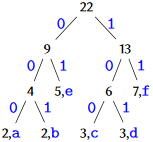
\includegraphics[scale=0.8]{images/Baum.PNG}
				\begin{tabular}{c c c c c c c}
					\textbf{Häufigkeiten:}\\
					\hline
					x  &a&b&c&d&e&f\\
					\hline
					$N_x(w)$& 2& 2&3&3& 5& 7\\
					\hline
				\end{tabular}	
			}
		\end{itemize} 
		\pause
		\item Ablesen der Codes aus dem Baum (Pfadbeschriftungen)
	\end{enumerate}
	\only<4>{
		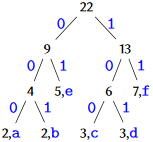
\includegraphics[scale=0.46]{images/Baum.png}
		\hspace{0.4cm}
		\begin{tabular}{c c c c c c c}
			\textbf{Häufigkeiten:}\\
			\hline
			x &a&b&c&d&e&f\\
			\hline
			$N_x(w)$ & 2& 2&3&3& 5& 7\\
			
			\textbf{Codewörter:}\\
			\hline
			x &a&b&c&d&e&f\\
			\hline
			h(x)& 000& 001&100&101& 01& 11\\
			\hline
		\end{tabular}							
	}		
\end{frame}

\begin{frame}{Übung zu Huffman Codierung}
	\begin{taskblock}{Übung}
		Sei $A = \{$\texttt a, b, c, d, e, f, g, h$\}$\\
		\begin{itemize}
			\item Codiere das Wort \texttt{badcfehg} mit Hilfe der Huffman-Codierung \pause
			\item [$\rightarrow$]Mögliche Lösung: 001 100 010 011 101 000 111 110
			\pause
			\item Wie lauten die Codewörter, wenn für das Wort $w$ gilt: $N_a(w) = 1, N_b(w) = 2, N_c(w) = 2, N_d(w) =8, N_e(w) =16, N_f(w) =32, N_g(w) = 64, N_h(w) = 128$
			
		\end{itemize} \pause
		Mögliche Lösung:\\
		\begin{tabular}{|c|c c c c c c c c|}
			\hline
			x &a&b&c&d&e&f&g&h\\
			\hline
			h(x)& 0000000& 0000001&000001&00001& 0001&001& 01&1\\
			\hline
		\end{tabular}
	\end{taskblock}
\end{frame}	

	\begin{frame}
	\begin{itemize}
		\item Wie lang wäre das zweite Wort (\texttt{abbcccc} $\texttt{d}^{8}$...$\texttt{g}^{64}\texttt{h}^{128}$) mit dem ersten Code codiert? 
		\pause
		\item[$\rightarrow$] 741 Symbole. Also dreimal so lang wie das Original. \pause
		\item Wie lang wäre das zweite Wort mit dem zweiten Code codiert?\pause
		\item[$\rightarrow$] 501 Symbole. Also nur zweimal so lang wie das Original. \pause
		\item Was fällt euch auf?
	\end{itemize}
\end{frame}		

\begin{frame}{Wahr oder falsch?}
	Sei $h: A^* \rightarrow \mathbb{Z}_2$ eine Huffman-Codierung
	\begin{itemize}
		\item h ist ein $\varepsilon$-freier Homomorphismus \pause \textbf{Wahr!}\pause
		\item Häufigere Symbole werden mit langen Worten codiert, seltene mit kürzeren \pause \textbf{Falsch!}\pause
		\item Die Kompression ist am stärksten, wenn die Häufigkeiten aller Zeichen ungefähr gleich sind. \pause \textbf{Falsch!} \pause
		\item h ist präfixfrei \pause \textbf{Wahr!} \pause
		\item Es kann noch kürzere Codierungen geben \pause \textbf{Falsch!}
	\end{itemize}
\end{frame}

	
\begin{frame}{Huffman-Codierung}
	\begin{block}{Eigenschaften}
		Sei $A$ ein Alphabet und $w \in A$. Dann gilt für die Huffman-Codierung h:
		\begin{itemize}
			\item $h: A^* \rightarrow \mathbb{Z}_2$
			\item $h$ ist $\varepsilon$-freier Homomorphismus
			\item $h$ ist präfixfreier Homomorphismus
			\item Häufigere Symbole werden mit kurzen Worten codiert, seltene mit längeren
			\item Produziert kürzestmögliche Codierungen
		\end{itemize}
	\end{block}
\end{frame}

\begin{frame}{Block-Codierung mit Huffman}
	\begin{itemize}
		\pitem Wir betrachten nicht mehr einzelne Symbole, sondern Blöcke von fester Länge $b > 1$
		\pitem Blätter des Huffman-Baums sind jetzt \textit{Wörter der Länge b}
	\end{itemize}

	\vspace{.5cm}
	
	Beispiel an der Tafel: Codierung von $aab\cdot deg \cdot deg \cdot aab \cdot ole \cdot aab \cdot deg \cdot aab$.\p
	
	\vspace{.5cm}
	
	\p
	\begin{itemize}
		\pitem Alphabet $A =\{$\texttt{a,b,c,d} $\}$
		\pitem Text über $A$, der nur aus Teilwörtern der Länge 10 zusammengesetzt ist, in denen jeweils immer nur ein Symbol vorkommt
		%\item z.B. \texttt{aaaaaaaaaabbbbbbbbbbcccccccccc}...
		\pitem Angenommen $\texttt{a}^{10}$, ..., $\texttt{d}^{10}$ kommen alle gleich häufig vor. Wie lang ist dann die Huffman-Codierung? \pause
		\pitem[$\rightarrow$] Ein Fünftel, weil jeder Zehnerblock durch zwei Bits codiert wird
	\end{itemize}
	
\end{frame}



\section{Speicher}


\begin{frame}{Speicher}
	\begin{itemize}
		\pitem Ein \textbf{Bit} ist Zeichen aus $A = \{0, 1\}$
		\pitem Ein \textbf{Byte} ist ein Wort aus acht Bits
		\pitem Abkürzungen
		\begin{itemize}
			\pitem Für Bit: \texttt{bit}
			\pitem Für Byte: \texttt{B}
		\end{itemize}
	\end{itemize}
\end{frame}

\begin{frame}{Präfixe}
	\begin{center}
		\textbf{Dezimal}\\
		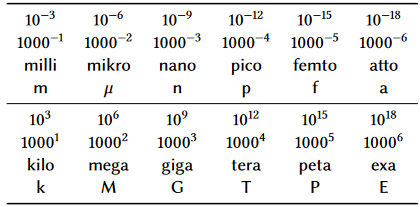
\includegraphics[scale=0.6]{images/dezimal.png}\\ \pause
		\textbf{Binär}\\
		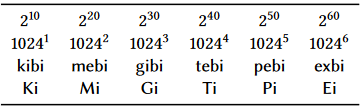
\includegraphics[scale=0.6]{images/binaer.png}
	\end{center}
	
\end{frame}

\begin{frame}{Gesamtzustand eines Speichers}
	\p Zu jedem Zeitpunkt ist
	\begin{itemize}
		\pitem für jede \markBlue{Adresse} festgelegt, welcher \markBlue{Wert} dort ist
		\pitem beides meist Bitfolgen
	\end{itemize}
	\p Vorstellung: Tabelle mit zwei Spalten\\
	\begin{center}
		\begin{tabular}{|l l|}
			\hline
			\textbf{Adresse} & \textbf{Wert} \\
			\hline
			Adresse 1& Wert 1 \\
			Adresse 2 & Wert 2 \\
			Adresse 3 & Wert 3 \\
			...&...\\
			Adresse n & Wert n\\
			\hline
		\end{tabular}
	\end{center}
\end{frame}

\begin{frame}{Zustand eines Speichers -- formal}
	\p\begin{block}{Definition des Speicherzustandes}
		Sei $Adr$ die Menge aller Adressen und $Val$ die Menge aller Werte.\\
		Dann ist \\ \begin{center}
			$m: Adr \rightarrow Val$
		\end{center}
		der aktuelle Zustand des Speichers. Dabei ist $m(a)$ der aktuelle Wert an der Adresse $a$.
	\end{block}
\end{frame}


\begin{frame}{Lesen und Speichern}
	\pause
	\begin{block}{$Mem$}
		Menge aller möglichen Speicherzustände, also Menge aller Abbildungen von $Adr$ nach $Val$
		\begin{center}
			$Mem:= Val^{Adr}$
		\end{center}
	\end{block}
	\p Anmerkung: \p Für zwei Mengen $A$, $B$ gilt\p : $A^B := \{f: B \rightarrow A\}$.\p
	\begin{block}{$memread$}
		\begin{center}
			$memread: Mem \times Adr \rightarrow Val \text{ mit } (m, a) \mapsto m(a)$
		\end{center}
	\end{block}
	\pause
	\begin{block}{$memwrite$}
		$memwrite: Mem \times Adr \times Val \rightarrow Mem \text{ mit } (m, a,v) \mapsto m'$\\
		Für $m'$ wird folgendes gefordert:
		\begin{center}
			$m(a') :=\begin{cases} 
			v& \text{ falls } a' = a\\
			m(a') &\text{ falls } a' \neq a
			\end{cases} $ 
		\end{center}
	\end{block}
\end{frame}

\begin{frame}{Eigenschaften von $memread$ und $memwrite$}
	
	\begin{block}{Eigenschaften (``Invarianten'')}
		\begin{itemize}
			\pitem $memread(memwrite(m,a,v),a) = v$ \p (Also: An $a$ einen Wert $v$ zu schreiben und danach bei $a$ zu lesen gibt den Wert $v$ zurück \p $\Rightarrow$ Konsistente Datenhaltung)
			\pitem $memread(memwrite(m, a', v'),a) = memread(m,a)$ \p (Also: Auslesen einer Speicherstelle ist unabhängig davon, was vorher an eine andere Adresse geschrieben wurde \p $\Rightarrow$ Unabhängige Datenhaltung)
		\end{itemize}
	\end{block}

\end{frame}

\begin{frame}
	\textbf{Aufgaben}\\
	Aktueller Speicherzustand: \\
	\vspace{0.2cm}
	\begin{tabular}{|c| c|}
		\hline
		Adresse & Wert\\
		\hline
		00000& 01110\\
		00001& 00100\\
		00010& 00111\\
		00011& 00000\\
		...& ...\\
		\hline
	\end{tabular}\\
	\vspace{0.3cm}
	Was ist?
	\begin{itemize}
		\item $memread(memwrite(m, memread(m, 00011), 01010), 00000)$ \pause
		\item[$\rightarrow$] 01010
	\end{itemize}
	
\end{frame}

\ifdefined\compileall
\else


\ifthenelse{\equal{\compiletype}{print}}
{

\begin{frame}{Informationen}
	
	\begin{columns}
		\begin{column}{0.5\textwidth}
			
			\begin{block}{Zum Tutorium}
				\begin{itemize}
					\item Lukas Bach
					\item Tutorienfolien auf: 
					\begin{itemize}
						\item \url{http://gbi.lukasbach.com}
					\end{itemize}
					\item Tutorium findet statt:
					\begin{itemize}
						\item Donnerstags, 14:00 - 15:30
						\item 50.34 Informatikbau, -107
					\end{itemize}
				\end{itemize}
			\end{block}
			
			\begin{block}{Mehr Material}
				\begin{itemize}
					\item Ehemalige GBI Webseite:
					\begin{itemize}
						\item \url{http://gbi.ira.uka.de}
						\item Altklausuren!
					\end{itemize}
				\end{itemize}
			\end{block}
			
		\end{column}
		\begin{column}{0.5\textwidth}
			
			\begin{block}{Zur Veranstaltung}
				\begin{itemize}
					\item Grundbegriffe der Informatik
					\item Klausurtermin:
					\begin{itemize}
						\item 06.03.2017, 11:00
						\item Zwei Stunden Bearbeitungszeit
						\item 6 ECTS für Informatiker und Informationswirte, 4 ECTS für Mathematiker und Physiker
					\end{itemize}
				\end{itemize}
			\end{block}
			
			\begin{block}{Zum Übungsschein}
				\begin{itemize}
					\item Übungsblatt jede Woche
					\item Ab 50\% insgesamt hat man den Übungsschein
					\item Keine Voraussetzung für die Klausur, aber für das Modul
				\end{itemize}
			\end{block}
			
		\end{column}
	\end{columns}
	
\end{frame}

}{}

\ifdefined\livebeamermode
	\begin{frame}
		
\includegraphics[width=\linewidth]{images/thatsall.png}
	\end{frame}
\fi

\end{document}

\fi
\def\tutdate{1.12.2016}

\ifdefined\compileall \else
\ifdefined\compiletype
	\documentclass[handout]{beamer}
\else
	\documentclass{beamer}
	\def\compiletype{livebeamer}
\fi

\usepackage{templates/beamerthemekitwide}

\usepackage[utf8]{inputenc}
\usepackage[T1]{fontenc}
\usepackage[ngerman]{babel}
\usepackage{listings}
\usepackage{hyperref}
\usepackage{graphicx}

\usepackage{amsmath}
\usepackage{amsthm}
\usepackage{amssymb}
\usepackage{polynom}

\usepackage{ifthen}
\usepackage{adjustbox} % for \adjincludegraphics

\newcommand{\markBlue}[1]{\textcolor{kit-blue100}{#1}}
\newcommand{\markGreen}[1]{\textcolor{kit-green100}{#1}}

\newcommand{\pitem}{\pause\item}
\newcommand{\p}{\pause}

% -- MATH MACROS
\newcommand{\thistheoremname}{}
\newcommand{\G}{\mathbb{Z}}
\newcommand{\B}{\mathbb{B}}
\newcommand{\R}{\mathbb{R}}
\newcommand{\N}{\mathbb{N}}
\newcommand{\Q}{\mathbb{Q}}
\newcommand{\C}{\mathbb{C}}
\newcommand{\Z}{\mathbb{Z}}
\newcommand{\F}{\mathbb{F}}
\newcommand{\mi}{\mathrm{i}}
\renewcommand{\epsilon}{\varepsilon}


\newenvironment<>{taskblock}[1]{%
	\setbeamercolor{block title}{fg=kit-orange15,bg=kit-orange100}
	\setbeamercolor{block body}{fg=black,bg=kit-orange30}%
	\begin{block}#2{#1}}{\end{block}}

\setbeamertemplate{enumerate items}[default]

% Aussagenlogik Symbole
\newcommand{\W}{w}
\renewcommand{\F}{f}

% Kodierung
\newcommand{\frepr}{\textbf{repr}}
\newcommand{\fRepr}{\textbf{Repr}}
\newcommand{\fZkpl}{\textbf{Zkpl}}
\newcommand{\fbin}{\textbf{bin}}
\newcommand{\fdiv}{\textbf{ div }}
\newcommand{\fmod}{\textbf{ mod }}

\title[Grundbegriffe der Informatik]{Grundbegriffe der Informatik\\Tutorium 33}
\subtitle{}
\author{Lukas Bach, lukas.bach@student.kit.edu}
\date{\tutdate}

\institute{}

\titlelogo{lukasbach}

\titleimage{bg}
%\titleimage{bg-advent}


\ifthenelse{\equal{\compiletype}{livebeamer}}
	{
		\def\livebeamermode{1}
	}{}

\ifthenelse{\equal{\compiletype}{print}}
	{
		\def\printmode{1}
	}{}

\setbeamercovered{invisible}

%\usepackage[citestyle=authoryear,bibstyle=numeric,hyperref,backend=biber]{biblatex}
%\addbibresource{templates/example.bib}
%\bibhang1em

\begin{document}
	
\selectlanguage{ngerman}


%title page
\begin{frame}
	\titlepage
\end{frame}

%table of contents
\ifdefined\printmode
	\ifdefined\compileall \else
	\begin{frame}{Gliederung}
		\tableofcontents
	\end{frame}
\fi\fi

\fi

% Zur Anpassung: Dekommentiere folgende Zeilen, um weniger \pause zu haben
% \renewcommand{\ip}{} % inline pause, für mitten im satz

% Dekommentiere folgende Zeilen, um Stil besser an deine Folien anzupassen
%\renewenvironment{taskblock}[1]{\textbf{Aufgabe: #1}\\}{}
%\renewcommand{\markBlue}[1]{\textbf{#1}}
%\renewcommand{\markGreen}[1]{\textbf{#1}}

% begin of slides

\section{Zum Übungsblatt}

\begin{frame}{Anmerkungen zum letzten Übungsblatt}
	\begin{itemize}
		\pitem Was ist sind die folgenden Mengen?
		\begin{itemize}
			\pitem $\N$ \pause = Menge der natürlichen Zahlen (1, 2, 3, ...)
			\pitem $\N_0$ \pause = $\N \cup \{0\}$
			\pitem $\R$ \pause = Menge der Reellen Zahlen
			\pitem $\R^+$ \pause = Menge der positiven reellen Zahlen
			\pitem $\R_0$ \pause gibt es nicht! $0$ ist auch so schon in $\R$
			\pitem $\R_0^+$ genauso nicht!
		\end{itemize}
		\pitem Aufgabe: $R: A^* \rightarrow A^*$
		\begin{itemize}
			\item $R(\epsilon) = \epsilon$
			\item $\forall x \in A: R(x) = x$
			\item $\forall w \in A^* \forall x \in A \forall y \in A: R(xwy) = yR(w)x$
			\item Zeige: $\forall n \in \N_0 : \forall w \in A^n: |R(w)| = |w|$
		\end{itemize}
	\end{itemize}
\end{frame}

\section{MIMA}

\begin{frame}{Was ist die MIMA?}
	\begin{itemize}
		\pitem Theoretischer, idealisierter Prozessor
		\pitem Funktioniert wie ein echter Prozessor, ist aber simpler
		\pitem Nah an Technischer Informatik
	\end{itemize}

	\bp
	
	Grundaufbau:
	
	\begin{itemize}
		\pitem Adressen als $20bit$ Datenwort
		\pitem Speicherworte als $24bit$ Datenwort
		\pitem Maschinenbefehle als...
		\begin{itemize}
			\item $4bit$ Befehl und $20bit$ Adresse
			\item oder $8bit$ Befehl und unwichtigem Rest
		\end{itemize}
	\end{itemize}
\end{frame}

\begin{frame}{Aufbau der MIMA: Steuerwerk}
	\begin{center}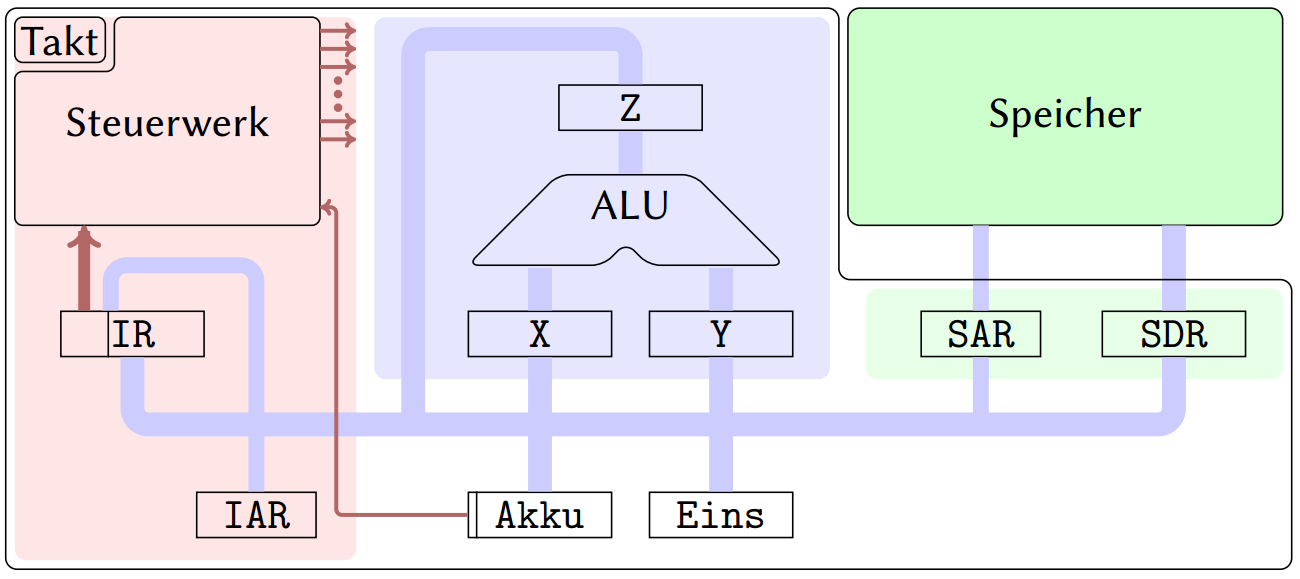
\includegraphics[width=.6\textwidth]{images/mima_aufbau.png}\end{center}
	
	\bp
	
	\textcolor{kit-red50}{\textbf{Steuerwerk}}
	
	\begin{columns}
		\begin{column}{0.5\textwidth}
			\begin{itemize}
				\pitem Instruction Register (IR) enthält den nächsten auszuführenden Befehl
				\pitem Instruction Adress Register (IAR) enthält die Adresse des nächsten Befehls
			\end{itemize}
		\end{column}
		
		\begin{column}{0.5\textwidth}
			\begin{itemize}
				\pitem Takt bestimmt die ``Tickrate'', also die Geschwindigkeit
				\pitem Steuerwerk interpretiert alle Befehle und führt sie aus
				\pitem Welche Befehle es gibt: Siehe später
			\end{itemize}
		\end{column}
	\end{columns}
	
\end{frame}


\begin{frame}{Aufbau der MIMA: Akku und Eins}
	\begin{center}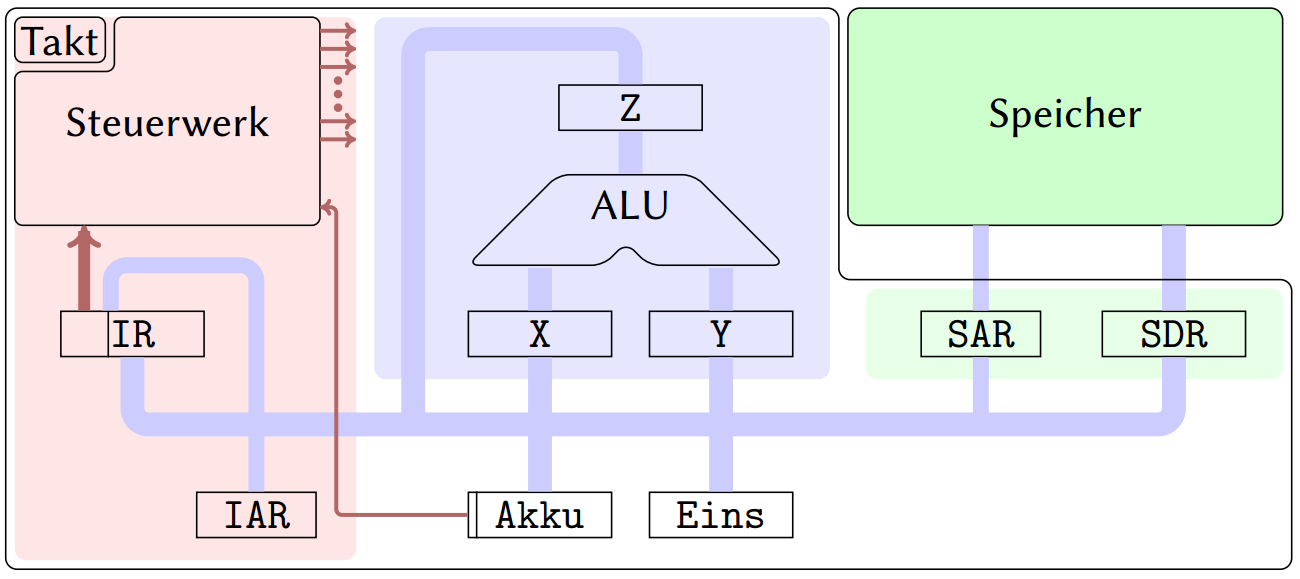
\includegraphics[width=.6\textwidth]{images/mima_aufbau.png}\end{center}
	
	\bp
	
	\textcolor{kit-orange50}{\textbf{Akku und Eins}}
	
	\begin{columns}
		\begin{column}{0.5\textwidth}
			\begin{itemize}
				\pitem Akku dient als Zwischenspeicher für Datenworte
				\pitem Hält maximal ein Wort
			\end{itemize}
		\end{column}
		
		\begin{column}{0.5\textwidth}
			\begin{itemize}
				\pitem Eins liefert die Konstante 1, hält also Strom
				\pitem z.B. erhöhen des IAR
			\end{itemize}
		\end{column}
	\end{columns}
	
\end{frame}


\begin{frame}{Aufbau der MIMA: ALU}
	\begin{center}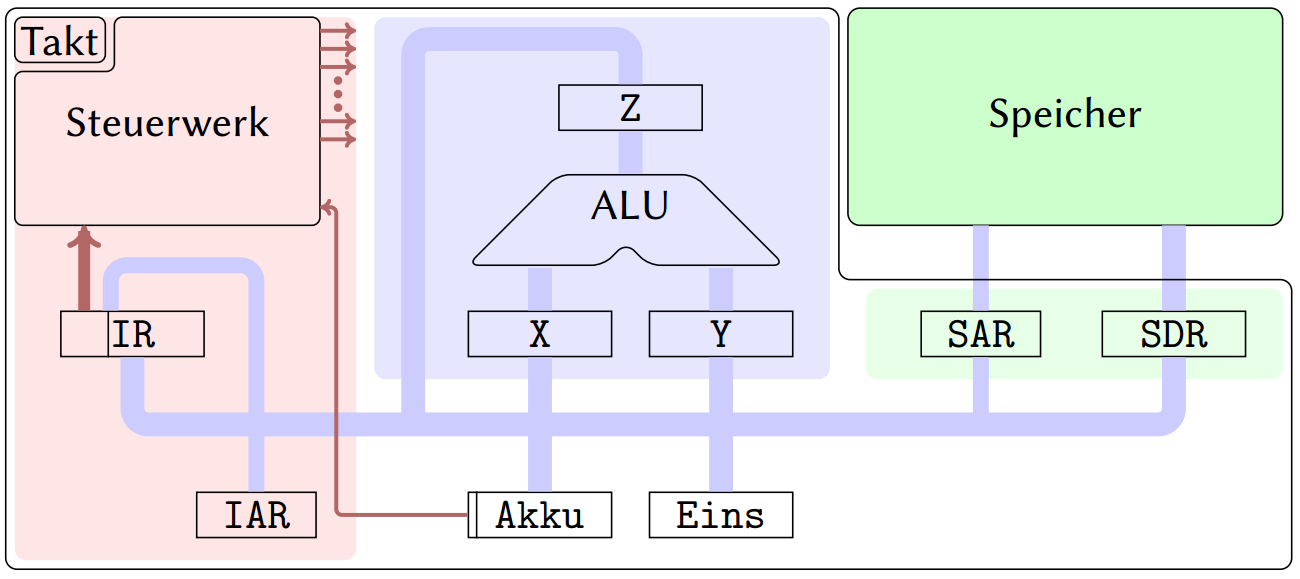
\includegraphics[width=.6\textwidth]{images/mima_aufbau.png}\end{center}
	
	\bp
	
	\textcolor{kit-blue50}{\textbf{Arithmetic Logic Unit (ALU) / Rechenwerk}}
	
	\begin{columns}
		\begin{column}{0.5\textwidth}
			\begin{itemize}
				\pitem Durchführt arithmetische Operationen
				\pitem $\fmod, \fdiv, +, -, ...$, bitweises OR/AND/...
			\end{itemize}
		\end{column}
		
		\begin{column}{0.5\textwidth}
			\begin{itemize}
				\pitem $X$ und $Y$ sind Eingaberegister
				\pitem $Z$ ist Ausgaberegister
			\end{itemize}
		\end{column}
	\end{columns}

\end{frame}


\begin{frame}{Aufbau der MIMA: ALU}
\begin{center}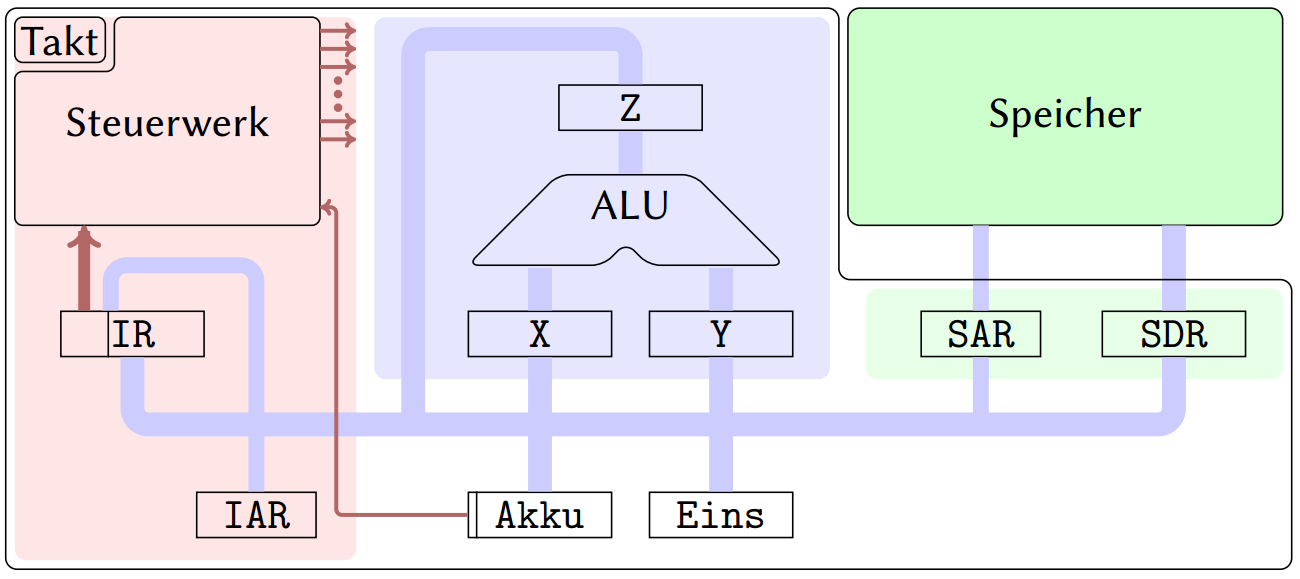
\includegraphics[width=.6\textwidth]{images/mima_aufbau.png}\end{center}

\bp

\textcolor{kit-green50}{\textbf{Speicher(werk)}}

Speicher selbst speichert Befehle und Daten. \ip Speicherwerk besteht aus:

\begin{columns}
	\begin{column}{0.5\textwidth}
		\begin{itemize}
			\pitem Speicheradressregister (SAR) ist die Adresse, bei der im Speicher gespeichert/gelesen werden soll
		\end{itemize}
	\end{column}
	
	\begin{column}{0.5\textwidth}
		\begin{itemize}
			\pitem Speicherdatenregister (SDR) Datum, das bei der Adresse gespeichert werden soll/ gelesen wurde.
		\end{itemize}
	\end{column}
\end{columns}

\end{frame}


\begin{frame}{Aufbau der MIMA: ALU}
\begin{center}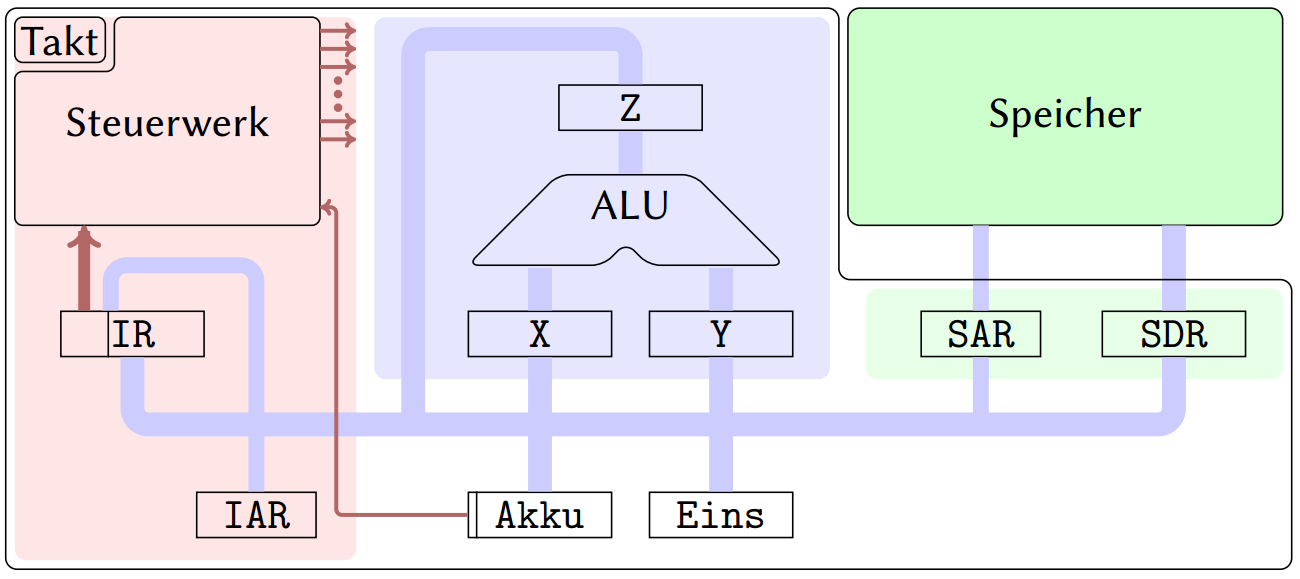
\includegraphics[width=.6\textwidth]{images/mima_aufbau.png}\end{center}

\bp

\textbf{Busse}

\begin{columns}
	\begin{column}{0.5\textwidth}
		\begin{itemize}
			\pitem ``Kabel'' zwischen den Verbindungen
			\pitem Ein kompletter Bus überträgt entweder $1$, $0$, oder nichts
		\end{itemize}
	\end{column}
	
	\begin{column}{0.5\textwidth}
		\begin{itemize}
			\pitem Kann nur eine einzige Information auf einmal übertragen
		\end{itemize}
	\end{column}
\end{columns}

\end{frame}

\begin{frame}{Konventionen zu MIMA Programmen}
	Um MIMA Programme und dazugehörige Definitionen verständlicher zu machen, vereinbaren wir folgende Konventionen:
	
	\bp
	
	\begin{itemize}
		\item Befehle (eigentlich Bitfolge) schreiben wir als Befehlname und Adresse
		\begin{itemize}
			\pitem $001000000000000000101010 \equiv STV$ $42$
		\end{itemize}
		\pitem $X \leftarrow Y \equiv $ ``Der Variable $X$ wird der Wert $Y$ zugewiesen''
		
	\end{itemize}
	
	
\end{frame}

\subsection{Maschinenbefehle}

% Folgende 3 Folien sollten nicht allzu ordentlich behandelt werden, mehr als vorzeitige Übersicht wieviele Befehle es gibt und als Referenz für die Tutanten für die Übungsaufgaben
\begin{frame}{MIMA Befehle}
	Eine MIMA-Maschine beherrscht folgende Maschinenbefehle:
	
	\vspace{.5cm}
	
	\begin{tabular}{r | l p{5cm} }
		Befehlssyntax & Formel & Bedeutung\\\hline\hline \ip
		$LDC$ $const$ & $Akku \leftarrow const$ & Lade eine Konstate $const$ in den Akku \\\hline \ip
		$LDV$ $adr$ & $Akku \leftarrow M(adr)$ & Lade einen Wert vom Speicher bei Adresse $adr$ in den Akku\\\hline\ip
		$STV$ $adr$ & $M(adr) \leftarrow Akku$ & Lade Speichere den Wert aus dem Akku im Speicher bei Adresse $adr$\\\hline\ip
		$LDIV$ $adr$ & $Akku \leftarrow M(M(adr))$ & Lade einen Wert vom Speicher bei der Adresse, die bei $adr$ gespeichert ist, und lade den Wert in den Akku\\\hline\ip
		$STIV$ $adr$ & $M(M(adr)) \leftarrow Akku$ & Speichere den Wert im Akku bei der Adresse, die in $adr$ gespeichert ist.
	\end{tabular}
\end{frame}

\begin{frame}{MIMA Befehle (2)}
	Eine MIMA-Maschine beherrscht folgende Maschinenbefehle:
	
	\vspace{.5cm}
	
	\begin{tabular}{r | l p{3cm} }
		Befehlssyntax & Formel & Bedeutung\\\hline\hline \ip
		$ADD$ $adr$ & $Akku \leftarrow Akku + M(adr)$ & Addiere den Wert bei $adr$ zum Akku dazu.\\\hline\ip
		$``OP''$ $adr$ & $Akku ``OP'' M(adr)$ & Wende bitweise Operation auf Akku mit Wert bei $adr$ an. $Op \in \{AND, OR, XOR\}$.
	\end{tabular}
\end{frame}

\begin{frame}{MIMA Befehle (3)}
	Eine MIMA-Maschine beherrscht folgende Maschinenbefehle:
	
	\vspace{.5cm}
	
	\begin{tabular}{r | p{8cm} }
		Befehlssyntax & Bedeutung\\\hline\hline \ip
		$NOT$ & Bitweise Invertierung aller Bits des Akku-Datenwortes\\\hline\ip
		$RAR$ & Rotiere alle Akku-Bits eins nach rechts\\\hline\ip
		$EQL$ $adr$ & Setze Akku auf $11\cdots11$, falls Wert bei $adr$ gleich Akku-Wert, setze Akku auf $00\cdots00$ sonst.\\\hline\ip
		$JMP$ $adr$ & Springe zu Befehlsadresse $adr$\\\hline\ip
		$JMN$ $adr$ & Springe zu Befehlsadresse $adr$, falls Akku negativ (also erstes Bit $=1$), sonst fahre normal fort.
	\end{tabular}
\end{frame}

% Bei folgenden Folien eventuell den Speicher auf die Tafel abschreiben und das Programm Befehl für Befehl durchgehen

% Laden und Speichern
\begin{frame}{MIMA Befehle: Sichern und Laden}
	\begin{itemize}
		\pitem Befehle zum laden und Speichern in den Speicher
		\pitem LDV um Daten vom Speicher zu laden, STV um Daten in den Speicher zu schreiben
		\pitem LDC um eine Konstante zu laden
		\pitem Daten werden in einem Zwischenspeicher gelagert, der nur ein Datenwort hält\ip : Akku.
	\end{itemize}

	\bp

	Beispiele:
	
	\begin{itemize}
		\pitem $LDV$ $9$ lädt das Datum, das im Speicher bei Adresse $9$ liegt, in den Akku.
		\pitem $STV$ $9$ speichert das Datum, das im Akku liegt, in den Speicher an Adresse $9$.
		\pitem $LDC$ $4$ lädt die Zahl $4$ in den Akku (also kein Speicherzugriff).
	\end{itemize}
\end{frame}

\begin{frame}{MIMA Befehle: Sichern und Laden}
	\begin{tabular}{r | l p{5cm} }
		Befehlssyntax & Formel & Bedeutung\\\hline\hline 
		$LDC$ $const$ & $Akku \leftarrow const$ & Lade eine Konstate $const$ in den Akku \\\hline 
		$LDV$ $adr$ & $Akku \leftarrow M(adr)$ & Lade einen Wert vom Speicher bei Adresse $adr$ in den Akku\\\hline
		$STV$ $adr$ & $M(adr) \leftarrow Akku$ & Lade Speichere den Wert aus dem Akku im Speicher bei Adresse $adr$\\\hline
	\end{tabular}

	\bp 
	\vspace{.5cm}
	\markGreen{Beispielprogramm mit initialem Speicherabbild}
	\vspace{.2cm}
	
	\begin{columns}
		\begin{column}{0.25\textwidth}
			LDC 5 \\ STV $a_1$ \\ LDC 7 \\ STV $a_2$ \\ $\vdots$
		\end{column}
		\begin{column}{0.25\textwidth}
			 $\vdots$ \\ LDV $a_1$ \\ STV $a_3$ \\ HALT
		\end{column}
		
		\begin{column}{0.5\textwidth}
			\begin{memory}
				\memrow{$a_1$}{0}	
				\memrow{$a_2$}{0}
				\memrow{$a_3$}{0}
			\end{memory}
		\end{column}
	\end{columns}

	%TODO Ergebnis
\end{frame}

% Laden und Speichern (indirekt)
\begin{frame}{MIMA Befehle: Indirektes Sichern und Laden}
	\begin{tabular}{r | l p{5cm} }
		Befehlssyntax & Formel & Bedeutung\\\hline\hline 
		$LDIV$ $adr$ & $Akku \leftarrow M(M(adr))$ & Lade einen Wert vom Speicher bei der Adresse, die bei $adr$ gespeichert ist, und lade den Wert in den Akku\\\hline
		$STIV$ $adr$ & $M(M(adr)) \leftarrow Akku$ & Speichere den Wert im Akku bei der Adresse, die in $adr$ gespeichert ist.
	\end{tabular}
	
	\bp 
	\vspace{.5cm}
	\markGreen{Beispielprogramm mit initialem Speicherabbild}
	\vspace{.2cm}
	
	\begin{columns}
		\begin{column}{0.5\textwidth}
			LDIV 4 \\ STV 5 \\ LDIV 5 \\ STIV 4 \\ HALT
		\end{column}
		
		\begin{column}{0.5\textwidth}
			\begin{memory}
				\memrow{$4$}{$6$}	
				\memrow{$5$}{$0$}
				\memrow{$6$}{$7$}
				\memrow{$7$}{$2$}
			\end{memory}
		\end{column}
	\end{columns}
\end{frame}

% Arithmetische Operationen
\begin{frame}{MIMA Befehle: Eins plus Eins}
	\begin{itemize}
		\pitem Befehle zu arithmetischen Operationen
		\pitem Eine ALU-Operation, angewandt auf dem Wert des Akkus und dem Wert an gegebener Adresse
		
		\bp
		
		\item Beispiele:
		\begin{itemize}
			\pitem $ADD$ $4$ addiert den Wert im Akku mit dem Wert aus dem Speicher an Adresse $4$ und legt das Resultat im Akku ab\ip . Achtung: Addition nicht mit dem Wert $4$!
			\pitem $AND$ $3$ führt bitweise Verundung zwischen dem Wert im Akku und dem Wert aus dem Speicher an Adresse $4$ durch und legt das Resultat im Akku ab.
		\end{itemize}
	\end{itemize}
\end{frame}


\begin{frame}{MIMA Befehle: Eins plus Eins}
	\begin{tabular}{r | l p{5cm} }
		Befehlssyntax & Formel & Bedeutung\\\hline\hline 
		$ADD$ $adr$ & $Akku \leftarrow Akku + M(adr)$ & Addiere den Wert bei $adr$ zum Akku dazu.\\\hline
		$``OP''$ $adr$ & $Akku ``OP'' M(adr)$ & Wende bitweise Operation auf Akku mit Wert bei $adr$ an. $Op \in \{AND, OR, XOR\}$.
	\end{tabular}
	
	\bp 
	\vspace{.5cm}
	\markGreen{Beispielprogramm mit initialem Speicherabbild}
	\vspace{.2cm}
	
	\begin{columns}
		\begin{column}{0.5\textwidth}
			LDC 5 \\ ADD 3 \\ AND 4 \\ STV 5 \\ LDC 12 \\ XOR 5 \\ HALT
		\end{column}
		
		\begin{column}{0.5\textwidth}
			\begin{memory}
				\memrow{$3$}{$3$}	
				\memrow{$4$}{$8$}
				\memrow{$5$}{$17$}
			\end{memory}
		\end{column}
	\end{columns}
\end{frame}

% Logische Operationen
\begin{frame}{MIMA Befehle: Bits und Bytes }
	\begin{itemize}
		\pitem $NOT$ invertiert alle Bits des Datums im Akku. \ip Beispiel $NOT$ mit $5$ im Akku, angenommen der Akku speichert bis zu 8 bits\ip : $5_{10} = 00000101_2$, nach der Invertierung: $1111 1010_2$.
		
		\pitem $RAR$ rotiert alle Bits des Datums im Akku um eine Stelle nach rechts. \ip Beispiel mit $5$ im Akku: $00000\markBlue{101}_2$ wird zu $\markBlue{1}00000\markBlue{10}_2$.
		
		\pitem $EQL$ $adr$ vergleicht den Wert im Akku mit dem Wert bei $addr$.
		\begin{itemize}
			\pitem Setzt Akku $= 11\cdots 11$ falls Werte gleich sind.
			\pitem Setzt Akku $= 00\cdots 00$ falls Werte nicht gleich sind.
		\end{itemize}
	\end{itemize}
\end{frame}
	
\begin{frame}{MIMA Befehle: Bits und Bytes }
	\begin{tabular}{r | p{8cm} }
		Befehlssyntax & Bedeutung\\\hline\hline 
		$NOT$ & Bitweise Invertierung aller Bits des Akku-Datenwortes\\\hline
		$RAR$ & Rotiere alle Akku-Bits eins nach rechts\\\hline
		$EQL$ $adr$ & Setze Akku auf $11\cdots11$, falls Wert bei $adr$ gleich Akku-Wert, setze Akku auf $00\cdots00$ sonst.\\\hline
	\end{tabular}
	
	\bp 
	\vspace{.5cm}
	\markGreen{Beispielprogramm mit initialem Speicherabbild}
	\vspace{.2cm}
	
	\begin{columns}
		\begin{column}{0.25\textwidth}
			LDC 5 \\ NOT \\ RAR \\ NOT \\ RAR \\ $\vdots$
		\end{column}
		\begin{column}{0.25\textwidth}
			$\vdots$ \\ RAR \\ EQL 15 \\ EQL 0 \\ HALT
		\end{column}
		
		\begin{column}{0.5\textwidth}
		\end{column}
	\end{columns}
\end{frame}

% Programmstruktur Operationen
\begin{frame}{MIMA Befehle: Springen}
	\begin{itemize}
		\pitem Normalerweise wird die Instruktionsadresse nach jedem Befehl um eins erhöht
		\pitem Also Befehle werden von oben nach unten abgearbeitet
		\pitem Mit Sprüngen kann man die MIMA zwingen, zu definiertem Befehl zu springen und damit die Vorgehensreihenfolge zu beeinflussen
		
		\vspace{.3cm} \bp
		
		\item $JMP$ $adr$ führt als nächsten Befehl den an Adresse $adr$ aus.
		\pitem $JMN$ $adr$ führt als nächsten Befehl den an Adresse $adr$ aus, \markGreen{falls der Akku negativ ist}.
		\begin{itemize}
			\pitem Also wenn das erste Bit im Akku negativ ist.
			\pitem Wenn vorher ein $EQL$ erfolgreich verglichen hat, wird also gesprungen.
			\pitem Wenn der Akku positiv ist, werden die Befehle nach $JMN$ normal weiter abgearbeitet.
		\end{itemize}
	\end{itemize}
\end{frame}
	
\begin{frame}{MIMA Befehle: Springen}
	\begin{tabular}{r | p{8cm} }
		Befehlssyntax & Bedeutung\\\hline\hline 
		$EQL$ $adr$ & Setze Akku auf $11\cdots11$, falls Wert bei $adr$ gleich Akku-Wert, setze Akku auf $00\cdots00$ sonst.\\\hline
		$JMP$ $adr$ & Springe zu Befehlsadresse $adr$\\\hline
		$JMN$ $adr$ & Springe zu Befehlsadresse $adr$, falls Akku negativ (also erstes Bit $=1$), sonst fahre normal fort.
	\end{tabular}
	
	\bp 
	\vspace{.5cm}
	\markGreen{Beispielprogramm mit initialem Speicherabbild}
	\vspace{.0cm}
	
	\begin{columns}
		\begin{column}{0.25\textwidth}
			\begin{align*}
				& \text{LDC 5} \\
				a_1: \quad  & \text{JMN } a_2 \\
				& \text{EQL 1} \\
				& \text{JMN } a_1 \\
				%& NOT \\ % sollte nicht erreicht sein
				%a_2: \quad & \text{JMP } a_3\\
				%& NOT \\ % sollte nicht erreicht sein
				%a_3: \quad & HALT
				\vdots
			\end{align*}
		\end{column}
		\begin{column}{0.25\textwidth}
			\begin{align*}
				%& \text{LDC 5} \\
				%a_1: \quad  & \text{JMN } a_2 \\
				%& \text{EQL 1} \\
				%& \text{JMN } a_1 \\
				\vdots \\
				& NOT \\ % sollte nicht erreicht sein
				a_2: \quad & \text{JMP } a_3\\
				& NOT \\ % sollte nicht erreicht sein
				a_3: \quad & HALT
			\end{align*}
		\end{column}
	
		\begin{column}{0.5\textwidth}
			\begin{memory}
				\memrow{$1$}{$5$}	
			\end{memory}
		\end{column}
	\end{columns}
\end{frame}

\subsection{Aufgaben}

\begin{frame}{Aufgaben}
	\begin{taskblock}{MIMA-Programm schreiben}
		Schreibe ein MIMA-Programm:
		\begin{itemize}
			\item Eingabe: Adresse $a_1$ einer positiven Zahl $x$.
			\item Ausgabe: Speichert $3 \cdot x$ in $a_1$.
		\end{itemize}
	\end{taskblock}
	
	\bp \vspace{.5cm} Lösung:
	
	LDV $a_1$ \\ ADD $a_1$ \\ ADD $a_1$ \\ STV $a_1$ \\ HALT
\end{frame}

\begin{frame}{Aufgaben}
	\begin{taskblock}{MIMA-Programm schreiben}
		Schreibe ein MIMA-Programm:
		\begin{itemize}
			\item Eingabe: Adresse $a_1$ einer positiven Zahl $x$.
			\item Ausgabe: Speichert $x \fmod 2$ in $a_1$.
		\end{itemize}
	\end{taskblock}

	\bp \vspace{.5cm} Lösung:
	
	LDC 1 \quad // 000000000000000000000001 \\ AND $a_1$ \\ STV $a_1$ \\ HALT
\end{frame}

\begin{frame}{Aufgaben}
	\begin{taskblock}{MIMA-Programm schreiben}
		Schreibe ein MIMA-Programm:
		\begin{itemize}
			\item Eingabe: Adresse $a_1$ einer positiven Zahl $x$.
			\item Ausgabe: Speichert $x \fdiv 2$ in $a_1$.
		\end{itemize}
	\end{taskblock}
	
	\bp \vspace{.5cm} Lösung:
	
	LDC 1 \\ NOT \\ AND $a_1$ \quad // Setze ``rechtestes'' Bit auf 0 \\ RAR \\ STV $a_1$ \\ HALT
\end{frame}

\ifdefined\compileall
\else


\ifthenelse{\equal{\compiletype}{print}}
{

\begin{frame}{Informationen}
	
	\begin{columns}
		\begin{column}{0.5\textwidth}
			
			\begin{block}{Zum Tutorium}
				\begin{itemize}
					\item Lukas Bach
					\item Tutorienfolien auf: 
					\begin{itemize}
						\item \url{http://gbi.lukasbach.com}
					\end{itemize}
					\item Tutorium findet statt:
					\begin{itemize}
						\item Donnerstags, 14:00 - 15:30
						\item 50.34 Informatikbau, -107
					\end{itemize}
				\end{itemize}
			\end{block}
			
			\begin{block}{Mehr Material}
				\begin{itemize}
					\item Ehemalige GBI Webseite:
					\begin{itemize}
						\item \url{http://gbi.ira.uka.de}
						\item Altklausuren!
					\end{itemize}
				\end{itemize}
			\end{block}
			
		\end{column}
		\begin{column}{0.5\textwidth}
			
			\begin{block}{Zur Veranstaltung}
				\begin{itemize}
					\item Grundbegriffe der Informatik
					\item Klausurtermin:
					\begin{itemize}
						\item 06.03.2017, 11:00
						\item Zwei Stunden Bearbeitungszeit
						\item 6 ECTS für Informatiker und Informationswirte, 4 ECTS für Mathematiker und Physiker
					\end{itemize}
				\end{itemize}
			\end{block}
			
			\begin{block}{Zum Übungsschein}
				\begin{itemize}
					\item Übungsblatt jede Woche
					\item Ab 50\% insgesamt hat man den Übungsschein
					\item Keine Voraussetzung für die Klausur, aber für das Modul
				\end{itemize}
			\end{block}
			
		\end{column}
	\end{columns}
	
\end{frame}

}{}

\ifdefined\livebeamermode
	\begin{frame}
		
\includegraphics[width=\linewidth]{images/thatsall.png}
	\end{frame}
\fi

\end{document}

\fi
\def\tutdate{8.12.2016}
\ifdefined\compileall \else
\ifdefined\compiletype
	\documentclass[handout]{beamer}
\else
	\documentclass{beamer}
	\def\compiletype{livebeamer}
\fi

\usepackage{templates/beamerthemekitwide}

\usepackage[utf8]{inputenc}
\usepackage[T1]{fontenc}
\usepackage[ngerman]{babel}
\usepackage{listings}
\usepackage{hyperref}
\usepackage{graphicx}

\usepackage{amsmath}
\usepackage{amsthm}
\usepackage{amssymb}
\usepackage{polynom}

\usepackage{ifthen}
\usepackage{adjustbox} % for \adjincludegraphics

\newcommand{\markBlue}[1]{\textcolor{kit-blue100}{#1}}
\newcommand{\markGreen}[1]{\textcolor{kit-green100}{#1}}

\newcommand{\pitem}{\pause\item}
\newcommand{\p}{\pause}

% -- MATH MACROS
\newcommand{\thistheoremname}{}
\newcommand{\G}{\mathbb{Z}}
\newcommand{\B}{\mathbb{B}}
\newcommand{\R}{\mathbb{R}}
\newcommand{\N}{\mathbb{N}}
\newcommand{\Q}{\mathbb{Q}}
\newcommand{\C}{\mathbb{C}}
\newcommand{\Z}{\mathbb{Z}}
\newcommand{\F}{\mathbb{F}}
\newcommand{\mi}{\mathrm{i}}
\renewcommand{\epsilon}{\varepsilon}


\newenvironment<>{taskblock}[1]{%
	\setbeamercolor{block title}{fg=kit-orange15,bg=kit-orange100}
	\setbeamercolor{block body}{fg=black,bg=kit-orange30}%
	\begin{block}#2{#1}}{\end{block}}

\setbeamertemplate{enumerate items}[default]

% Aussagenlogik Symbole
\newcommand{\W}{w}
\renewcommand{\F}{f}

% Kodierung
\newcommand{\frepr}{\textbf{repr}}
\newcommand{\fRepr}{\textbf{Repr}}
\newcommand{\fZkpl}{\textbf{Zkpl}}
\newcommand{\fbin}{\textbf{bin}}
\newcommand{\fdiv}{\textbf{ div }}
\newcommand{\fmod}{\textbf{ mod }}

\title[Grundbegriffe der Informatik]{Grundbegriffe der Informatik\\Tutorium 33}
\subtitle{}
\author{Lukas Bach, lukas.bach@student.kit.edu}
\date{\tutdate}

\institute{}

\titlelogo{lukasbach}

\titleimage{bg}
%\titleimage{bg-advent}


\ifthenelse{\equal{\compiletype}{livebeamer}}
	{
		\def\livebeamermode{1}
	}{}

\ifthenelse{\equal{\compiletype}{print}}
	{
		\def\printmode{1}
	}{}

\setbeamercovered{invisible}

%\usepackage[citestyle=authoryear,bibstyle=numeric,hyperref,backend=biber]{biblatex}
%\addbibresource{templates/example.bib}
%\bibhang1em

\begin{document}
	
\selectlanguage{ngerman}


%title page
\begin{frame}
	\titlepage
\end{frame}

%table of contents
\ifdefined\printmode
	\ifdefined\compileall \else
	\begin{frame}{Gliederung}
		\tableofcontents
	\end{frame}
\fi\fi

\fi

\section{Kontextfreie Grammatiken}
\begin{frame}{Kontextfreie Grammatiken}
	\ip Zur Rekapitulation...
	
	\begin{itemize}
		\pitem Was ist ein Alphabet, was eine formale Sprache?
		\pitem Was kennen wir für Operationen auf formalen Sprachen?
	\end{itemize}

	\bp 
	
	Betrachte $L := \{a^nba^n : n \in \N \}$. \ip Wie kann man diese Sprache darstellen?
\end{frame}

\begin{frame}{Kontextfreie Grammatiken}
	\begin{block}{Kontextfreie Grammatik}
		Ein Tupel G = (N, T, S, P) mit
		\begin{itemize}
			\pitem $N$ Alphabet (Nichtterminalsymbole)
			\pitem $T$ Alphabet mit $N \cap T = \emptyset$ (Terminalsymbole)
			\pitem $S \in N$ (Startsymbol)
			\pitem $P \subseteq N \times (N \cup T)^* \text{ mit } |P| \in \mathbb{N}_0$
		\end{itemize}
	\end{block}

	\begin{itemize}
		\pitem Was ist $N \times (N \cup T)^*$? \pause Bei $N := \{a,b,c\}, T = \{S, A, B\}$\ip : $N \times (N \cup T)^* = \{(a, abSAcB), (a, SSS), (b, BSabc), ...\}$.
		\pitem Andere Schreibweise: $P : N \rightarrow (N \cup T)^*$.
		\pitem Für $(X, w) \in P$ schreibt man $X \rightarrow w$
		\pitem Statt $\{X\rightarrow w_1, X \rightarrow w_2 \}$ schreibt man auch $\{X \rightarrow w_1 | w_2\}$
	\end{itemize}
	
\end{frame}

\begin{frame}{Ableitungsschritt}
	Erinnerung: $N = Nichtterminalsymbole$, $T = Terminalsymbole$. \pause
	
	\begin{block}{Ableitungsschritt}
		\ip $v \in (N \cup T)^*$  \ip ist in einem Schritt aus $u \in (N \cup T)^*$ ableitbar\ip , wenn 
		\begin{itemize}
			\pitem $u = w_1 X w_2 \text{ und } v = w_1 w_X w_2 \text{ für } w_1, w_2 \in (N \cup T)^* $
			\pitem und $X \rightarrow w_X$ in $P$
		\end{itemize}
	\end{block}

	\bp\markBlue{Notation}\\
	$u\Rightarrow v$\\
	\bp\markBlue{Beispiel}\\
	$G:= (\{S,B\}, \{a,b\}, S, \{S \rightarrow aBa|aSa, B \rightarrow b\})$
	
	\begin{itemize}
		\pitem $S \ip\Rightarrow aSa \ip\Rightarrow aaSaa \ip\Rightarrow aaaBaaa \ip\Rightarrow aaabaaa$. \ip Fertig.
		\pitem $aaaSaaa \not\Rightarrow aaaabaaaa$! \ip $\Rightarrow$ heißt \markGreen{eine} Ableitung!
	\end{itemize}
\end{frame}

\begin{frame}{Ableitungsfolge}
	\bp
	\begin{block}{Ableitungsfolge}
		Wir definieren $\Rightarrow^i$ für $i \in \mathbb{N}_0$ folgendermaßen:\\\vspace{.3cm}
		\bp Für $u,v \in (N \cap T)^*$ gelte:
		\begin{itemize}
			\pitem $u \Rightarrow^0 v$ genau dann, wenn $u = v$ gilt.
			\pitem $u \Rightarrow^{i+1} v$ genau dann, wenn ein $w \in (N \cup T)^* $ existiert, für das $u \Rightarrow w \Rightarrow^i v$ gilt.
			Für $u \Rightarrow^i v$ sagt man "\markGreen{v ist aus $u$ in $i$ Schritten ableitbar}".
		\end{itemize}
	\end{block}

	\bp

	\textbf{Beispiel}\\
	$G:= (\{S,B\}, \{a,b\}, S, \{S \rightarrow aBa|aSa, B \rightarrow b\})$\\
	\ip Dann gilt $aaaSaaa \Rightarrow^0 aaaSaaa$ \ip \\
	und $aaaSaaa \Rightarrow^2 aaaabaaaa$
\end{frame}

\begin{frame}\bp
	\begin{block}{Ableitbarkeit}
		Für $u,v \in (N \cup T)^*$ gelte $u \Rightarrow^* v$ \ip genau dann, wenn ein $i \in \mathbb{N}_0$ existiert\ip , mit $u \Rightarrow^i v$. \ip Man sagt dann "\markGreen{v ist aus u ableitbar}".
	\end{block}\bp
	\textbf{Beispiel}\\
	$G:= (\{S,B\}, \{a,b\}, S, \{S \rightarrow aBa|aSa, B \rightarrow b\})$\\
	\ip Dann gilt $S \Rightarrow^* aaaSaaa$ \ip \\
	und $aSa \Rightarrow^* aaaabaaaa$ \ip \\
	aber $aSa \not\Rightarrow abba$.
\end{frame}

\begin{frame}{Ableitungsbaum}
	\begin{columns}
		\begin{column}{0.5\textwidth}
			\begin{itemize}
				\pitem Startsymbol ist Wurzel
				\pitem Nichtterminale sind innere Knoten
				\pitem Für $X \Rightarrow w $ sind die Zeichen von $w$ die Kinder von X
				\pitem Terminale sind die Blätter
			\end{itemize}
		\end{column}
		
		\begin{column}{0.5\textwidth}\bp
			\textbf{Beispiel}\\
			$G:= (\{S,B\}, \{a,b\}, S, \{S \rightarrow aBa|aSa, B \rightarrow b\})$\bp\\
			Dann gilt $S \Rightarrow^* aaabaaa$\\
			\center 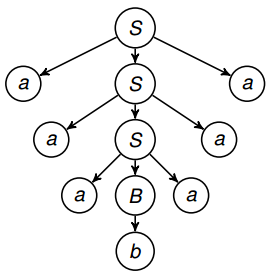
\includegraphics[scale=0.7]{images/Ableitungsbaum.png}
		\end{column}
	\end{columns}
	
\end{frame}

\begin{frame}{Übung zu Kontextfreien Grammatiken}
	\begin{taskblock}{Übung}
		Gegeben ist die Kontextfreie Grammatik (N, T, S, P) mit:
		
		\begin{itemize}
			\item Nichtterminalsymbolen $N := \{A, B, S\}$.
			\item Terminalsymbolen $T := \{a, b, c\}$
			\item Startsymbol $S$
			\item Produktionen $P := \{S \rightarrow aaS | bbS | SAS | \epsilon, A \rightarrow cB , B \rightarrow a, b, c, \epsilon\}$.
		\end{itemize}
	
		\bp
	
		Aufgabe: Welche der folgenden Wörter sind ableitbar? Konstruiere den Ableitungsbaum und zeige, wie sie abgeleitet werden.
		
		\begin{itemize}
			\item $ccbbcbbbbcbbaaaa$? %ja
			\item $aabbaabbaabb$? %ja
			\item $c$?
		\end{itemize}
	\end{taskblock}
\end{frame}

\begin{frame}{Formale Sprachen erzeugen}
	\bp\begin{block}{Erzeugte Sprache}
		Sei $G = (N, T, S, P)$ eine kontextfreie Grammatik. \ip Dann nennen wir $L(G) := \{w \in T^*| S \Rightarrow^* w\}$ die von G erzeugte Sprache.
	\end{block}

	\bp
	
	\begin{block}{Kontextfreie Sprache}
		Eine formale Sprache $L$ heißt genau dann kontextfrei, wenn eine kontextfreie Grammatik $G$ existiert, mit $L(G) = L$.
	\end{block}

	\bp

	$G:= (\{S,B\}, \{a,b\}, S, \{S \rightarrow aBa|aSa, B \rightarrow b\})$\\\vspace{.3cm}
	\ip Dann ist $L(G) = \{a^nba^n|n \in \mathbb{N_+}\}$
\end{frame}

\begin{frame}{Verständnisfragen}
	\begin{itemize}
		\item $G = (\{X\}, \{a,b\}, X, \{X \rightarrow \varepsilon| aX| bX\})$
		\begin{itemize}
			\item Welche Wörter lassen sich in drei Schritten ableiten?
			\pause		 		
			\item[$\rightarrow$] $\{aa, ab, ba, bb\}$
			\pause
			\item Was ist $L(G)$?
			\pause		 		
			\item[$\rightarrow$] $L(G) = \{a,b\}^*$
		\end{itemize}
		\pause
		\item Gibt es auch eine Grammatik $G$ mit $L(G) = \{\}$?
		\pause
		\item[$\rightarrow$] $G_1 := (\{X\}, \{a,b\}, X, \{X\rightarrow X\})$ oder $G_2 := (\{X\}, \{a,b\}, X, \{\})$
		\pause
		\item Wahr oder falsch? Wenn $w_1 \Rightarrow w_2$ gilt, dann gilt auch $w_1 \rightarrow w_2$
		\pause
		\item Was ist der Unterschied von $\Rightarrow$ und $\Rightarrow^*$ ?
	\end{itemize}
\end{frame}

\begin{frame}
	\begin{taskblock}{Aufgaben zu kontextfreien Grammatiken}
		\begin{itemize}
			\item Sei $L_1 := \{wbaaw'|w, w' \in \{a,b\}^*\}$. Konstruiere eine Grammatik $G_1$ mit $L(G_1) = L_1$.
			\pause
			\item[$\rightarrow$] $G_1 := (\{X, Y\}, \{a,b\}, X, \{X \rightarrow YbaaY, Y \rightarrow aY|bY|\varepsilon\})$.
			\pause
			\item  Welche Sprache erzeugt $ G_2 = (\{S, X, Y\}, \{a,b\}, S, P_2)$  mit $P_2 = \{S \rightarrow X|Y, X \rightarrow aaXb|aab, Y \rightarrow aYbb|abb\}$?
			\pause			
			\item[$\rightarrow$] $L(G_2) = \{a^{2k}b^{k} | k \in \mathbb{N}_+\} \cup \{a^kb^{2k}| k \in \mathbb{N}_+\}$
			%\pause
			%\item Sei $L_3 := \{w \in \{a,b\}^*| \forall \text{ Präfixe } v \text{ von } w : |N_a(v) - N_b(v)| \leq 1 \}$. Konstruiere eine Grammatik $G_3$ mit $L(G_3) = L_3$
			%\pause
			%\item[$\rightarrow$] $G_3 = (\{X\}, \{a,b\}, X, \{X\rightarrow abX|baX|a|b|\varepsilon\})$
		\end{itemize}
	\end{taskblock}	
\end{frame}

\begin{frame}{Beispiel zu kontextfreien Grammatiken}
	$G= (\{X\}, \{\textcolor{blue}{(}, \textcolor{blue}{)}\}, X, \{X \rightarrow XX|\textcolor{blue}{(} X \textcolor{blue}{)}| \varepsilon\} )$
	\begin{itemize}
		\pitem Welche Wörter sind ableitbar?
		\pause
		\item[$\rightarrow$] "wohlgeformte Klammerausdrücke"
		\pause
		\item Welche Eigenschaften besitzen diese Wörter?
		\pause
		\item[$\rightarrow$]$N_{\textcolor{blue}{(}}(w) = N_{\textcolor{blue}{)}}(w)$ \pause Ist diese Eigenschaft hinreichend?
		\pause
		\item[$\rightarrow$]Nein, es muss gelten: Für alle Präfixe $v$ von $w$ gilt $ N_{\textcolor{blue}{(}}(v) \geq N_{\textcolor{blue}{)}}(v)$
		\pause
		\item Andere Grammatik möglich, die alle wohlgeformten Klammerausdrücke erzeugt?
		\pause
		\item[$\rightarrow$]  $G= (\{X\}, \{\textcolor{blue}{(}, \textcolor{blue}{)}\}, X, \{X \rightarrow \textcolor{blue}{(} X \textcolor{blue}{)}X| \varepsilon\} )$
	\end{itemize}
\end{frame}

\begin{frame}{Grenze kontextfreier Grammatiken}
	Es gibt auch Sprachen, die wir nicht mit einer kontextfreien Grammatik erzeugen können!
	
	\vspace{.3cm} \bp
	Beispiel aus der Vorlesung:\\
	$L_{vv} = \{vcv| v \in \{a,b\}^*\} \subseteq \{a, b, c\}^*$
\end{frame}


\section{Relationen vol. 2}
\begin{frame}{Relationen}
	\pause
	\begin{block}{Erinnerung Relationen}
		Es seien A und B Mengen. \ip Eine Teilmenge $R \subseteq A \times B$ heißt Relation.
	\end{block}
\end{frame}

\begin{frame}
	\bp
	
	\begin{block}{Definition Produkt von Relationen}
		Es seinen $A, B \text{ und  } C$ Mengen und $R \subseteq A \times B, S \subseteq B \times C$ Relationen. Dann ist \\$S \circ R := \{(a,c) \in A \times C | \text{ } \exists b \in B \text{ mit } (a,b) \in R \land (b,c) \in S\}$ \\
		das Produkt der Relationen $R$ und $S$.
	\end{block}
	\bp\textbf{Bemerkung}\\
	\ip $S \circ R$ ist eine Relation auf $A$ und $C$\ip , bildet also von $A$ nach $C$ ab.
	\bp\begin{block}{Assoziativität des Produktes}
		Es seien $ A, B, C$ und $D$ Mengen und $R \subseteq A \times B, S \subseteq B \times C$ sowie $T \subseteq C \times D$ Relationen. \ip Dann gilt\ip \\
		$(T \circ S) \circ R = T \circ (S \circ R)$.
	\end{block}
\end{frame}

\begin{frame}
	\bp\begin{block}{Homogene Relation}
		Es seien A und B Mengen und $R \subseteq A \times B$ eine Relation. \ip $R$ heißt homogen, wenn $A=B$ und heterogen, wenn $A \neq B $ gilt.
	\end{block}
	
	\bp\begin{block}{Identität}
		Sei $M$ eine Menge. $I_M := \{(x,x)| x \in M\}$		
	\end{block}

	\bp\begin{block}{Potenz von Relationen}
		Sei $M$ eine Menge und $R \subseteq M  \times M$ eine homogene Relation. \ip Dann definieren wir $R^i$ für $i \in \mathbb{N}_0$ folgendermaßen: 
		\begin{itemize}
			\pitem $R^0 := I_M$
			\pitem Für alle $i \in \mathbb{N}_0: R^{i+1} := R^i \circ R$
		\end{itemize}
	
		\ip Also $R^4 = R \circ R \circ R \circ R$.
	\end{block}
\end{frame}

\begin{frame}{Reflexitivität}
	\bp\begin{block}{Satz über das neutrale Element}
		Es seien $A$ und $B$ Mengen und $R \subseteq A \times B$ eine Relation. Dann gilt: $R \circ I_B = R = I_A \circ R$.
	\end{block}
	
	\bp\begin{block}{Reflexivität}
		Sei M eine Menge und $R \subseteq M \times M$ eine homogene Relation. Wenn für alle $x \in M: (x,x) \in R$, nennt man $R$ reflexiv.
		
		\ip Also jedes Element der Definitionsmenge der Relation wird auf sich selbst abgebildet (und vielleicht auch auf andere Elemente abgebildet).
	\end{block}
	
	\bp\begin{block}{Lemma}
		Sei $M$ eine Menge und $R \subseteq M \times M$ eine homogene Relation. $R$ ist genau dann reflexiv, wenn $I_M \subseteq R$ gilt.
	\end{block}
\end{frame}

\begin{frame}{Transitivität}
	\bp\begin{block}{Transitivität}
		Sei $M$ eine Menge und $R \subseteq M \times M$ eine homogene Relation. \\ \ip R heißt transitiv, wenn: \ip\\ $\forall x, y, z \in M: (x,y) \in R \land (y, z) \in R \rightarrow (x,z) \in R$
	\end{block}
	
	\bp\begin{block}{Lemma}
		Sei $M$ eine Menge und $R \subseteq M \times M$ eine homogene Relation. $R$ ist genau dann transitiv, wenn $R \circ R \subseteq R$.
	\end{block}
\end{frame}

\begin{frame}
	\textbf{Aufgaben}\\
	Sei $M := \{1, 2, 3 \}$.
	\begin{itemize}
		\item Ist $R:= \{(1,1), (1,2), (2,3)\}$ transitiv? \pause Nein!
		\pause
		\item Ist $R$ reflexiv? \pause Nein!
		\pause
		\item Wie müsste R aussehen, um transitiv zu sein?
		\pause
		\item Ist $S:= \{(1,1), (1,2), (1,3), (2,2), (2,3)\}$ reflexiv? \pause Nein!
		\pause
		\item Ist $S$ transitiv? \pause \hspace{0.3cm} Ja!
		\item Wie müsste S aussehen, um reflexiv zu sein?
	\end{itemize}
\end{frame}

\begin{frame}{Reflexiv-transitive Hülle}
	\bp\begin{block}{Definition}
		Sei M eine Menge und $R \subseteq M \times M$ eine homogene Relation. \\Dann nennt man $R^* := \bigcup\limits_{i \in \mathbb{N}_0} R^i$ die reflexiv-transitive Hülle von R.
	\end{block}
	\bp\begin{block}{Satz}
		\begin{itemize}
			\item $R^*$ ist reflexiv
			\item $R^*$ ist transitiv
			\item $R^*$ ist die kleinste Relation, die reflexiv und transitiv ist und $R \subseteq R^*$ erfüllt.
		\end{itemize}
	\end{block}
	\bp\textbf{Bemerkung}\\
	\begin{itemize}
		\item Sei M eine Menge und $R\subseteq M \times M$ eine homogene, reflexive und transitive Relation. Dann gilt $R^* = R$.
	\end{itemize}
	
\end{frame}
\begin{frame}
	\textbf{Aufgaben}\\
	\begin{itemize}
		\item Sei $M = \{1, 2, 3\}$ und $R := \{(1,1), (1,2), (2,3)\}$ Was ist $R^*$?
		\pause
		\item[$\rightarrow$] $R^* = \{(1,1), (1,2), (1,3), (2,2), (2,3), (3,3)\}$ 
		\pause
		\item Sei $M$ eine Menge und $R \subseteq M \times M$ eine homogene Relation. Was ist $(R^*)^*$ ?
		\pause
		\item[$\rightarrow$]  $(R^*)^* = R^*$
		\pause
		\item $M := \{1,2,3,4\} \text{ und } R := \{(1,2), (2,3), (3,4), (4,1)\} \subseteq M \times M$. Ist R reflexiv? Ist R transitiv? \pause \hspace{0.3cm} Nein und nein!
	\end{itemize}
\end{frame}

\begin{frame}
	Die Relationen $R$ und $S$ über $\mathbb{N}_0$ seien gegeben durch:
	\begin{itemize}
		\item Für alle $a, b \in \mathbb{N}_0: aRb \Leftrightarrow a|b$ ($a$ ist Teiler von $b$)
		\item Für alle $a, b \in \mathbb{N}_0: aSb \Leftrightarrow ggT(a,b) = 1$ 
	\end{itemize}
	Prüfe auf Reflexivität und Transitivität!
	\pause
	\begin{itemize}
		\item[$\rightarrow$] R ist transitiv, aber nicht reflexiv.
		\pause
		\item[$\rightarrow$] S ist reflexiv, aber nicht transitiv. [TODO]
	\end{itemize}
\end{frame}
\ifdefined\compileall
\else


\ifthenelse{\equal{\compiletype}{print}}
{

\begin{frame}{Informationen}
	
	\begin{columns}
		\begin{column}{0.5\textwidth}
			
			\begin{block}{Zum Tutorium}
				\begin{itemize}
					\item Lukas Bach
					\item Tutorienfolien auf: 
					\begin{itemize}
						\item \url{http://gbi.lukasbach.com}
					\end{itemize}
					\item Tutorium findet statt:
					\begin{itemize}
						\item Donnerstags, 14:00 - 15:30
						\item 50.34 Informatikbau, -107
					\end{itemize}
				\end{itemize}
			\end{block}
			
			\begin{block}{Mehr Material}
				\begin{itemize}
					\item Ehemalige GBI Webseite:
					\begin{itemize}
						\item \url{http://gbi.ira.uka.de}
						\item Altklausuren!
					\end{itemize}
				\end{itemize}
			\end{block}
			
		\end{column}
		\begin{column}{0.5\textwidth}
			
			\begin{block}{Zur Veranstaltung}
				\begin{itemize}
					\item Grundbegriffe der Informatik
					\item Klausurtermin:
					\begin{itemize}
						\item 06.03.2017, 11:00
						\item Zwei Stunden Bearbeitungszeit
						\item 6 ECTS für Informatiker und Informationswirte, 4 ECTS für Mathematiker und Physiker
					\end{itemize}
				\end{itemize}
			\end{block}
			
			\begin{block}{Zum Übungsschein}
				\begin{itemize}
					\item Übungsblatt jede Woche
					\item Ab 50\% insgesamt hat man den Übungsschein
					\item Keine Voraussetzung für die Klausur, aber für das Modul
				\end{itemize}
			\end{block}
			
		\end{column}
	\end{columns}
	
\end{frame}

}{}

\ifdefined\livebeamermode
	\begin{frame}
		
\includegraphics[width=\linewidth]{images/thatsall.png}
	\end{frame}
\fi

\end{document}

\fi
\def\tutdate{15.12.2016}
\ifdefined\compileall \else
\ifdefined\compiletype
	\documentclass[handout]{beamer}
\else
	\documentclass{beamer}
	\def\compiletype{livebeamer}
\fi

\usepackage{templates/beamerthemekitwide}

\usepackage[utf8]{inputenc}
\usepackage[T1]{fontenc}
\usepackage[ngerman]{babel}
\usepackage{listings}
\usepackage{hyperref}
\usepackage{graphicx}

\usepackage{amsmath}
\usepackage{amsthm}
\usepackage{amssymb}
\usepackage{polynom}

\usepackage{ifthen}
\usepackage{adjustbox} % for \adjincludegraphics

\newcommand{\markBlue}[1]{\textcolor{kit-blue100}{#1}}
\newcommand{\markGreen}[1]{\textcolor{kit-green100}{#1}}

\newcommand{\pitem}{\pause\item}
\newcommand{\p}{\pause}

% -- MATH MACROS
\newcommand{\thistheoremname}{}
\newcommand{\G}{\mathbb{Z}}
\newcommand{\B}{\mathbb{B}}
\newcommand{\R}{\mathbb{R}}
\newcommand{\N}{\mathbb{N}}
\newcommand{\Q}{\mathbb{Q}}
\newcommand{\C}{\mathbb{C}}
\newcommand{\Z}{\mathbb{Z}}
\newcommand{\F}{\mathbb{F}}
\newcommand{\mi}{\mathrm{i}}
\renewcommand{\epsilon}{\varepsilon}


\newenvironment<>{taskblock}[1]{%
	\setbeamercolor{block title}{fg=kit-orange15,bg=kit-orange100}
	\setbeamercolor{block body}{fg=black,bg=kit-orange30}%
	\begin{block}#2{#1}}{\end{block}}

\setbeamertemplate{enumerate items}[default]

% Aussagenlogik Symbole
\newcommand{\W}{w}
\renewcommand{\F}{f}

% Kodierung
\newcommand{\frepr}{\textbf{repr}}
\newcommand{\fRepr}{\textbf{Repr}}
\newcommand{\fZkpl}{\textbf{Zkpl}}
\newcommand{\fbin}{\textbf{bin}}
\newcommand{\fdiv}{\textbf{ div }}
\newcommand{\fmod}{\textbf{ mod }}

\title[Grundbegriffe der Informatik]{Grundbegriffe der Informatik\\Tutorium 33}
\subtitle{}
\author{Lukas Bach, lukas.bach@student.kit.edu}
\date{\tutdate}

\institute{}

\titlelogo{lukasbach}

\titleimage{bg}
%\titleimage{bg-advent}


\ifthenelse{\equal{\compiletype}{livebeamer}}
	{
		\def\livebeamermode{1}
	}{}

\ifthenelse{\equal{\compiletype}{print}}
	{
		\def\printmode{1}
	}{}

\setbeamercovered{invisible}

%\usepackage[citestyle=authoryear,bibstyle=numeric,hyperref,backend=biber]{biblatex}
%\addbibresource{templates/example.bib}
%\bibhang1em

\begin{document}
	
\selectlanguage{ngerman}


%title page
\begin{frame}
	\titlepage
\end{frame}

%table of contents
\ifdefined\printmode
	\ifdefined\compileall \else
	\begin{frame}{Gliederung}
		\tableofcontents
	\end{frame}
\fi\fi

\fi

% pop quiz

\section{Prädikatenlogik}
\begin{frame}{Grundlagen zu Prädikatenlogik}
	Prädikatenlogik (PL) \ip \markBlue{erweitert} Aussagenlogik durch Ergänzen von ``Prädikaten''\ip , einer Art von Funktionen, die Wahrheitswerte zurückgeben.
	
	\bp
	
	Alphabet der Prädikatenlogik:
	
	\begin{itemize}
		\pitem $\lnot, \land, \lor, \rightarrow, \leftrightarrow, (, )$, also Alphabet der Aussagenlogik.
		\pitem $\forall$ Allquantor \ip ($\forall x$ heißt ``für alle $x$ gilt...)
		\pitem $\exists$ Existenzquantor \ip ($\exists x$ heißt ``es existiert min. ein $x$... für das gilt...)
		\pitem $x,y,z,x_i \in Var_{PL}$ Variablen
		\pitem $c, d, c_i \in Const_{PL}$ Konstanten
		\pitem $f, g, h, f_i \in Fun_{PL}$ Funktionen %TODO Selligkeit ar(f_i) = anzahl parameter
		\pitem $R, S, R_i \in Rel_{PL}$ Relationen (funktionieren ähnlich wie Funktionen)
		\pitem $\objequiv$ Objektgleichheit
		\pitem $,$ Komma
	\end{itemize}
\end{frame}

\begin{frame}{Gliederung der Prädikatenlogik}
	\begin{block}{Terme}
		Ein Term ist ein Element aus der Sprache über $A_{Ter} := \{\markBlue{(}, \markBlue{)}, \markBlue{,}\} \cup Var_{PL} \cup Const_{PL} \cup Fun_{PL}$.
	\end{block}

	\bp
	
	\begin{block}{Atomare Formeln}
		Atomare Formeln sind zum Beispiel
		\begin{itemize}
			\pitem Objektgleichheiten $f_1 \objequiv f_2$
			\pitem Relation von Termen $R(t_1, t_2, ...)$
		\end{itemize}
	\end{block}

	\begin{block}{Stelligkeit einer Funktion}
		Die Stelligkeit $ar(f) \in \N_+$ einer Funktion gibt die Anzahl der Parameter von $f$ an. \ip (Analog Stelligkeit von Relationen $ar(R)$)
	\end{block}
	
	%\bp
\end{frame}

\begin{frame}{Verständnis von Termen, Atomaren Formeln, Stelligkeit}
\begin{itemize}
	\item Woraus kann ein Term bestehen? \pause
	\item[$\rightarrow$] Aus Klammern $\markBlue{(}, \markBlue{)}$, Kommas $\markBlue{,}$, Variablen, Konstanten, Funktionen.\pause
	\item Was davon sind atomare Formeln: $R(x) \land S(f(x, c))$, $R(x, g(c, f(y, x))$?\pause
	\item[$\rightarrow$] Nein, ja.\pause
	\item Was sind die Stelligkeiten folgender Funktionen: $f(a, b, c), g(a), h(a, b)$? \pause \item[$\rightarrow$] $4,1,2$.
\end{itemize}	
\end{frame}

\begin{frame}{Grammatik der Prädikatenlogik}
	Prädikatenlogische Formeln werden durch die Grammatik $G := (N_{Ter}, A_{Ter}, T, P_{Ter})$ erzeugt mit:
	
	\bp
	
	\begin{itemize}
		\pitem $m+1$ Nichtterminalsymbolen $N_{Ter} := \{T\} \cup \{L_i | i \in \N_+ \text{ und } i \leq m \}$ ($m = $ Maximale Stelligkeit von Funktionen)
		\pitem Terminalsymbolen: Alphabet, aus dem Terme erzeugbar sind
		%\pitem Startsymbol $T$
		\pitem Produktionen
		\begin{alignat*}{2}
		L_{i+1} &\to L_i , T &\qquad& \text{für jedes } i\in\N_+\text{ mit } i<m   \\
		L_1  &\to T \\ % ACHTUNG Komma ist hier ein Terminalsymbol, kein Trennsymbol
		T &\to c_i && \text{für jedes } c_i\in Const_{PL}\\
		T &\to x_i && \text{für jedes } x_i\in Var_{PL}\\
		T &\to f_i(L_{ar(f_i)} ) && \text{für jedes } f_i\in Fun_{PL}
		\end{alignat*}
	\end{itemize}

	\bp
	
	Beispiel: Seien Funktionen $f,g$ mit $ar(f) = 2, ar(g) = 1$, Konstante $c$ und Variablen $x,y$ gegeben. Was kann man damit machen?
\end{frame}

\begin{frame}{Grammatik der Prädikatenlogik}
	
	
	\begin{columns}
		\begin{column}{0.6\textwidth}
			Beispiel: Seien Funktionen $f,g$ mit $ar(f) = 2, ar(g) = 1$, Konstante $c$ und Variablen $x,y$ gegeben. Was kann man damit machen?\vspace{.2cm}
			
			\bp
			
			Dann: 
			\begin{itemize}
				\item $N_{Ter}=\{ T, L_1, L_2 \}$
				\item $\begin{aligned}[t]
				P_{Ter} = \{  L_2 & \to L_1 , T \\% ACHTUNG Komma ist hier ein Terminalsymbol, kein Trennsymbol
				L_1 & \to T  \\
				T   & \to c \\
				T   & \to x \\
				T   & \to y \\
				T   & \to g ( L_1 ) \\
				T   & \to f ( L_2 ) \}
				\end{aligned}
				$
			\end{itemize}
		\end{column}
		
		\begin{column}{0.4\textwidth}
			\bp
			
			\begin{taskblock}{Aufgabe zu Grammatiken und Prädikatenlogik}
				Welche dieser Formeln entsprechen dieser Grammatik?
				\vspace{.2cm}
				\begin{itemize}
					\pitem $f(c, g(x))$
					\pitem $f(x, y, c)$
					\pitem $g(f(c, c))$
					\pitem $g(g(f(g(x), g(f(c, c))))$
					\pitem $g(c\ip, f)c)$
				\end{itemize}
			
				\ip Bilde die Ableitungsbäume zu den korrekten Formeln.
			\end{taskblock}
		\end{column}
	\end{columns}
\end{frame}

\begin{frame}{Bindungsstärken}
	\begin{block}{Bindungsstärke}
		Verschiedene Operanden ``binden'' stärker als andere. \ip Wenn ein Operand stärker als die umliegenden Operanden bindet, tritt derselbe Effekt auf, wie wenn Klammerung geschehen würde.
	\end{block}

	\bp
	
	Bindungsstärken absteigen:
	\begin{itemize}
		\ip \item $\forall / \exists\ip,\lnot\ip,\land\ip,\lor\ip,\rightarrow/\leftarrow\ip,\leftrightarrow$
	\end{itemize}

	\bp
	
	Finde äquivalente Formeln, die mit möglichst wenig Klammern auskommen:
	\begin{itemize}
		\pitem $\exists x \forall y (R(f(x), g(x)) \lor \forall z R(c, x)$ %TODO finish
	\end{itemize}

\end{frame}

\begin{frame}{Interpretation von prädikatenlogischen Formeln}
	
\end{frame}

\begin{frame}

\end{frame}

\ifdefined\compileall
\else


\ifthenelse{\equal{\compiletype}{print}}
{

\begin{frame}{Informationen}
	
	\begin{columns}
		\begin{column}{0.5\textwidth}
			
			\begin{block}{Zum Tutorium}
				\begin{itemize}
					\item Lukas Bach
					\item Tutorienfolien auf: 
					\begin{itemize}
						\item \url{http://gbi.lukasbach.com}
					\end{itemize}
					\item Tutorium findet statt:
					\begin{itemize}
						\item Donnerstags, 14:00 - 15:30
						\item 50.34 Informatikbau, -107
					\end{itemize}
				\end{itemize}
			\end{block}
			
			\begin{block}{Mehr Material}
				\begin{itemize}
					\item Ehemalige GBI Webseite:
					\begin{itemize}
						\item \url{http://gbi.ira.uka.de}
						\item Altklausuren!
					\end{itemize}
				\end{itemize}
			\end{block}
			
		\end{column}
		\begin{column}{0.5\textwidth}
			
			\begin{block}{Zur Veranstaltung}
				\begin{itemize}
					\item Grundbegriffe der Informatik
					\item Klausurtermin:
					\begin{itemize}
						\item 06.03.2017, 11:00
						\item Zwei Stunden Bearbeitungszeit
						\item 6 ECTS für Informatiker und Informationswirte, 4 ECTS für Mathematiker und Physiker
					\end{itemize}
				\end{itemize}
			\end{block}
			
			\begin{block}{Zum Übungsschein}
				\begin{itemize}
					\item Übungsblatt jede Woche
					\item Ab 50\% insgesamt hat man den Übungsschein
					\item Keine Voraussetzung für die Klausur, aber für das Modul
				\end{itemize}
			\end{block}
			
		\end{column}
	\end{columns}
	
\end{frame}

}{}

\ifdefined\livebeamermode
	\begin{frame}
		
\includegraphics[width=\linewidth]{images/thatsall.png}
	\end{frame}
\fi

\end{document}

\fi
\def\tutdate{22.12.2016}
\ifdefined\compileall \else
\ifdefined\compiletype
	\documentclass[handout]{beamer}
\else
	\documentclass{beamer}
	\def\compiletype{livebeamer}
\fi

\usepackage{templates/beamerthemekitwide}

\usepackage[utf8]{inputenc}
\usepackage[T1]{fontenc}
\usepackage[ngerman]{babel}
\usepackage{listings}
\usepackage{hyperref}
\usepackage{graphicx}

\usepackage{amsmath}
\usepackage{amsthm}
\usepackage{amssymb}
\usepackage{polynom}

\usepackage{ifthen}
\usepackage{adjustbox} % for \adjincludegraphics

\newcommand{\markBlue}[1]{\textcolor{kit-blue100}{#1}}
\newcommand{\markGreen}[1]{\textcolor{kit-green100}{#1}}

\newcommand{\pitem}{\pause\item}
\newcommand{\p}{\pause}

% -- MATH MACROS
\newcommand{\thistheoremname}{}
\newcommand{\G}{\mathbb{Z}}
\newcommand{\B}{\mathbb{B}}
\newcommand{\R}{\mathbb{R}}
\newcommand{\N}{\mathbb{N}}
\newcommand{\Q}{\mathbb{Q}}
\newcommand{\C}{\mathbb{C}}
\newcommand{\Z}{\mathbb{Z}}
\newcommand{\F}{\mathbb{F}}
\newcommand{\mi}{\mathrm{i}}
\renewcommand{\epsilon}{\varepsilon}


\newenvironment<>{taskblock}[1]{%
	\setbeamercolor{block title}{fg=kit-orange15,bg=kit-orange100}
	\setbeamercolor{block body}{fg=black,bg=kit-orange30}%
	\begin{block}#2{#1}}{\end{block}}

\setbeamertemplate{enumerate items}[default]

% Aussagenlogik Symbole
\newcommand{\W}{w}
\renewcommand{\F}{f}

% Kodierung
\newcommand{\frepr}{\textbf{repr}}
\newcommand{\fRepr}{\textbf{Repr}}
\newcommand{\fZkpl}{\textbf{Zkpl}}
\newcommand{\fbin}{\textbf{bin}}
\newcommand{\fdiv}{\textbf{ div }}
\newcommand{\fmod}{\textbf{ mod }}

\title[Grundbegriffe der Informatik]{Grundbegriffe der Informatik\\Tutorium 33}
\subtitle{}
\author{Lukas Bach, lukas.bach@student.kit.edu}
\date{\tutdate}

\institute{}

\titlelogo{lukasbach}

\titleimage{bg}
%\titleimage{bg-advent}


\ifthenelse{\equal{\compiletype}{livebeamer}}
	{
		\def\livebeamermode{1}
	}{}

\ifthenelse{\equal{\compiletype}{print}}
	{
		\def\printmode{1}
	}{}

\setbeamercovered{invisible}

%\usepackage[citestyle=authoryear,bibstyle=numeric,hyperref,backend=biber]{biblatex}
%\addbibresource{templates/example.bib}
%\bibhang1em

\begin{document}
	
\selectlanguage{ngerman}


%title page
\begin{frame}
	\titlepage
\end{frame}

%table of contents
\ifdefined\printmode
	\ifdefined\compileall \else
	\begin{frame}{Gliederung}
		\tableofcontents
	\end{frame}
\fi\fi

\fi

\section{Algorithmen}
\begin{frame}{Algorithmen}
	\begin{itemize}
		\pitem Es existiert eine \textbf{endliche} Beschreibung
		\pitem Es wird zu einer beliebig großen, aber \textbf{endlichen} Eingabe eine \textbf{endliche} Ausgabe berechnet
		\pitem Es finden \textbf{endlich} viele Schritte statt (der Algorithmus terminiert)
		\pitem Deterministisch (bei mehrmaliger Ausführung kommt immer das selbe raus)
	\end{itemize}
\end{frame}

\subsection{Pseudocode}
\begin{frame}{Hier verwendeter Pseudocode}
	\begin{itemize}
		\pitem Zuweisungssymbol $\leftarrow$
		\pitem Schlüsselwörter für Verzweigungen \textbf{if, then, else, fi}
		\pitem Schlüsselwörter für Schleifen \textbf{while, do, od, for, to}
		\pitem Symbole für Konstanten, Funktionen und Relationen
	\end{itemize}
\end{frame}

\begin{frame}
	Eine \textbf{if}-Verzweigung\\
	\vspace{0.2cm}
	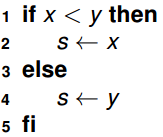
\includegraphics[scale=0.6]{images/if.png}\\
	\vspace{0.2cm}\p
	Eine \textbf{while}-Schleife\\
	\vspace{0.2cm}
	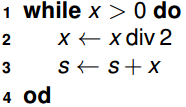
\includegraphics[scale=0.6]{images/while.png}\\
	\vspace{0.2cm}\p
	Eine \textbf{for}-Schleife\\
	\vspace{0.2cm}
	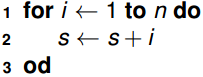
\includegraphics[scale=0.6]{images/for.png}
\end{frame}

\begin{frame}{Was kann man mit Algorithmen machen?}
	\begin{itemize}
		\pitem Komplexe Algorithmen mit Pseudocode definieren zu Sortierung, Graphen, Datenstrukturen\ip, im Modul \markBlue{Algorithmen I}
		\pitem Laufzeitanalyse von Algorithmen\ip, später.
		\pitem Korrektheitsbeweise\ip, jetzt.
	\end{itemize}
\end{frame}

\begin{frame}{Korrektheitsbeweise}
	\ip Wie findet man heraus, ob ein Algorithmus korrekt funktioniert?
	\begin{itemize}
		\pitem Durch den Beweis von Zusicherungen, die an bestimmten Stellen des Algorithmus gelten.
	\end{itemize}

	\vertspace

	\bp Was sind Zusicherungen?
	\begin{itemize}
		\pitem prädikatenlogische Formeln, die Aussagen über (Zusammenhänge zwischen) Variablen machen
	\end{itemize}
\end{frame}



%	\begin{frame}
%	\textbf{Beispiel}\\
%	Was ist hier die Schleifeninvariante?\\
%	\vspace{0.1cm}
%		Seien $a,b \in \mathbb{N}_0$\\
%		$x \leftarrow b$\\
%		$x \leftarrow a$\\
%		$while$ $y \neq 0$\\
%		do \\
%		\hspace{0.4cm} $y \leftarrow y - 1$\\
%		\hspace{0.4cm} $x \leftarrow x + 1$\\
%		od
%	\end{frame}


\subsection{Das Hoare-Kalkül}
\begin{frame}{Das Hoare-Tripel}
	\p
	
	\begin{block}{Definition}
		$\{P\}S\{Q\}$ heißt Hoare-Tripel. \ip Dabei gilt:
		\begin{itemize}
			\pitem S ist ein Programmstück im Pseudocode
			\pitem P und Q sind Zusicherungen
		\end{itemize}
	\end{block}
	\begin{itemize}
		\pitem P nennt man Vorbedingung, Q Nachbedingung
		\pitem Prädikatenlogische Formeln
		\pitem Beispiel (Vorausblick): $\{x \objequiv  1 \} x \leftarrow x + 1 \{x \objequiv 2\}$
		\pitem Meistens in jeder Zeile nur eine Zeile Code oder ein Zusicherungsblock
	\end{itemize}
\end{frame}

\begin{frame}{Das Hoare-Tripel}
	\begin{block}{Gültigkeit von Hoare-Tripeln}
		$\{P\}S\{Q\}$ ist gültig, wenn für jede gültige Interpretation $(D, I)$ und Variablenbelegung $\beta$ gilt:\\\bp
		Aus 
		\begin{itemize}
			\pitem $val_{D, I, \beta}(P) = w$
			\pitem $\beta'$ ist Variablenbelegung nach Ausführung von $S$
		\end{itemize}
		\ip folgt $val_{D, I, \beta'}(Q) = w$
	\end{block}
\end{frame}

\begin{frame}{Zuweisung}
	\begin{block}{Axiom HT-A}
		\begin{itemize}
			\pitem Sei $x \leftarrow E$ eine Zuweisung
			\pitem $Q$ eine Nachbedingung von $x \leftarrow E$ und
			\pitem $\sigma_{\{x/E\}}$ kollisionsfrei für Q
		\end{itemize}
		\p Dann ist $\sigma_{\{x/E\}}(Q) x \leftarrow E\{Q\}$ ein gültiges Hoare-Tripel
	\end{block}\p
	\textbf{Bemerkung}\\
	\begin{itemize}
		\pitem $\sigma_{\{x/E\}}$ ist die Substitution von $x$ mit $E$
		\pitem Bei Anwendung der Regel rückwärts vorgehen
	\end{itemize}
\end{frame}

\begin{frame}
	\textbf{Beispiel}\\
	Betrachte die Zuweisung \\
	$x \leftarrow x +1$\\
	und die Nachbedingung\\
	$\{x \dot = 1\}$\\
	\ip Nach HT-A gilt\\
	\pause
	$\{x+1 \dot = 1\}$ $ x \leftarrow x + 1$ $ \{x \dot = 1\}$ ist ein gültiges Hoare-Tripel.
\end{frame}

\begin{frame}{Ableitungsregeln: HT-E}
	\begin{itemize}
		\item Verstärkung der Vorbedingung
		\item Abschwächung der Nachbedingung
	\end{itemize}\p
	\begin{block}{HT-E}
		Wenn $\{P\}S\{Q\}$ ein gültiges Hoare-Tripel ist und $P' \vdash P$ und $Q \vdash Q'$ gelten, dann folgt:\\
		\pause
		$\{P'\}S \{Q'\}$ ist ein gültiges Hoare-Tripel.
	\end{block}
	\p\textbf{Bemerkung}\\
	$B \vdash A :\Leftrightarrow$ Aussage $A$ ist syntaktisch aus Aussage $B$ ableitbar
\end{frame}

\begin{frame}
	\textbf{Beispiel}\\
	Angenommen es sei $\{y > 3\}$ $x \leftarrow y-1$ $\{x > 1\}$ ein gültiges Hoare-Tripel.\\
	Es gilt $\{(y>4)\} \vdash \{(y>3)\} $ und $\{(x>1)\} \vdash \{(x>0)\} $.\\
	Also folgt nach HT-E:\\
	\pause
	$\{y > 4\}$ $x \leftarrow y-1$ $\{x > 0\}$ ist ein gültiges Hoare-Tripel.\\
	\pause
	\vertspace
	\textbf{Bemerkung}\\
	Es müssen sich nicht unbedingt beide Bedingungen ändern! \\
	Aus $\{(y>3)\} \vdash \{(y>3)\} $ und $\{(x>1)\} \vdash \{(x>0)\} $ \\folgt nach HT-E auch \\
	$\{y > 3\}$ $x \leftarrow y-1$ $\{x > 0\}$ ist ein gültiges Hoare-Tripel.
\end{frame}

\begin{frame}{Ableitungsregeln: HT-S}
	\p Hintereinanderausführung von durch Hoare-Triple bewiesene Code Segmente sind selbst gültig.\p
	\begin{block}{HT-S}
		Wenn $\{P\}S_1\{Q\}$ und $\{Q\}S_2\{R\}$ gültige Hoare-Tripel sind\ip, dann folgt:\ip $\{P\}S_1; S_2\{R\}$ ist ein gültiges Hoare-Tripel. 
	\end{block}
	\p\textbf{Bemerkung}\\
	";"  \space trennt hier zwei Programmstücke
\end{frame}

\begin{frame}
	\textbf{Beispiel}\\
	Angenommen es seien $\{y > 3\}$ $x \leftarrow y-1$ $\{x > 1\}$ und \\
	$\{x > 1\}$ $z \leftarrow x-1$ $\{z > -1\}$ gültige Hoare-Tripel.\\
	\ip Dann folgt nach HT-S:\\
	\pause
	$\{y > 3\}$ $x \leftarrow y-1; z \leftarrow x-1$ $\{z > -1\}$ ein gültiges Hoare-Tripel.
\end{frame}

\begin{frame} {Bedingte Anweisungen}\p
	\begin{block}{HT-I}
		Wenn $\{P \land B\}S_1\{Q\}$ und $\{P \land \lnot B\}S_2\{Q\}$ gültige Hoare-Tripel sind\ip, dann folgt:\\
		
		\vertspace
		\quad$\{P\}$\\
		\qquad\textbf{if} $B$ \textbf{then} $S_1$ \\
		\qquad\textbf{else} $S_2$\\
		\qquad\textbf{fi}\\
		\quad$\{Q\}$\\
		\vertspace
		
		
		ist ein gültiges Hoare-Tripel.
	\end{block}
\end{frame}

\begin{frame}{Beispiel}
	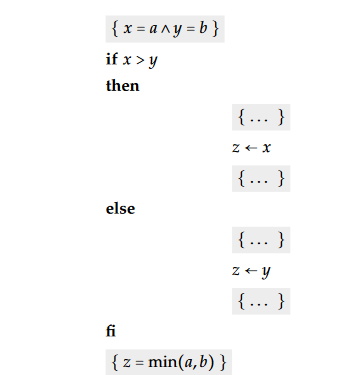
\includegraphics[scale=0.6]{images/if_fi.PNG}
\end{frame}		

\begin{frame}{Beispiel}
	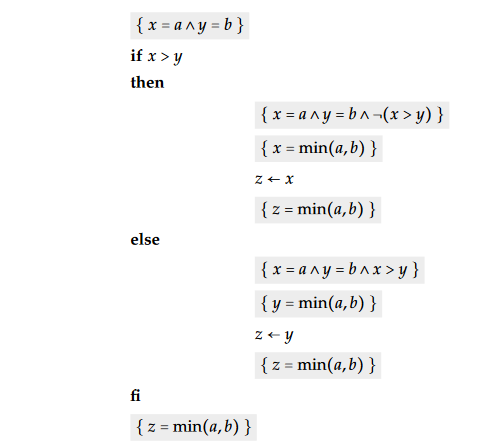
\includegraphics[scale=0.6]{images/if_fi_loes.PNG}
\end{frame}		

%\begin{frame}{Weiteres Beispiel}
%Sei $p$ eine Person, $betrunken(p)$ ein einstelliges Prädikat mit $betrunken(p) = wahr %:\Leftrightarrow getrunkeneGl"uhweins \objequiv 20$.
%\begin{algorithm}
%	$\{getrunkeneGl"uhweins = 0\}$
%	\While{$\lnot betrunken(p)$}{$getrunkeneGl"uhweins \leftarrow getrunkeneGl"uhweins + 1$}
%\end{algorithm}
%\end{frame}

\begin{frame} {Schleifen}
	\begin{block}{HT-W}
		Wenn $\{I \land B\}S\{I\}$ ein gültiges Hoare-Tripel ist\ip, dann folgt:\\\ip
		
		\vertspace
		$\{I\}$\\
		\textbf{while} $B$
		\textbf{do} $S$ \\
		\textbf{od}\\
		$\{I \land \lnot B\}$\\
		\vertspace
		
		ist ein gültiges Hoare-Tripel.
	\end{block}
\end{frame}

\begin{frame}{Schleifeninvariante}
	\begin{itemize}
		\pitem Eine spezielle Zusicherung
		\pitem Schleifeninvarianten müssen \textbf{vor}, \textbf{während} und \textbf{nach} jedem Schleifendurchlauf gelten
		\pitem Garantiert, dass die Schleife nicht während einem beliebigen Durchlauf ``kaputt'' geht.
		%\pitem Sie \textbf{müssen nicht} während des Schleifendurchlaufs gelten (können aber)
	\end{itemize}
\end{frame}

\begin{frame}
	\textbf{Beispiel}\\
	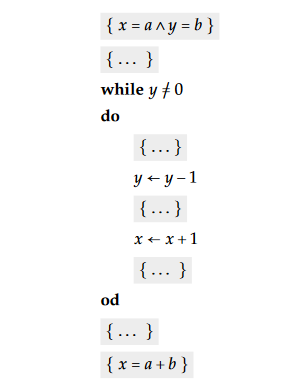
\includegraphics[scale=0.7]{images/do_od.PNG}
\end{frame}

\begin{frame}
	\textbf{Beispiel}\\
	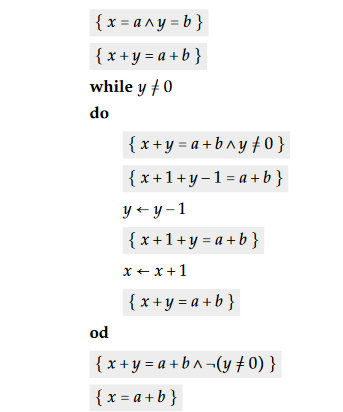
\includegraphics[scale=0.7]{images/do_od_loes.png}
\end{frame}
\ifdefined\compileall
\else


\ifthenelse{\equal{\compiletype}{print}}
{

\begin{frame}{Informationen}
	
	\begin{columns}
		\begin{column}{0.5\textwidth}
			
			\begin{block}{Zum Tutorium}
				\begin{itemize}
					\item Lukas Bach
					\item Tutorienfolien auf: 
					\begin{itemize}
						\item \url{http://gbi.lukasbach.com}
					\end{itemize}
					\item Tutorium findet statt:
					\begin{itemize}
						\item Donnerstags, 14:00 - 15:30
						\item 50.34 Informatikbau, -107
					\end{itemize}
				\end{itemize}
			\end{block}
			
			\begin{block}{Mehr Material}
				\begin{itemize}
					\item Ehemalige GBI Webseite:
					\begin{itemize}
						\item \url{http://gbi.ira.uka.de}
						\item Altklausuren!
					\end{itemize}
				\end{itemize}
			\end{block}
			
		\end{column}
		\begin{column}{0.5\textwidth}
			
			\begin{block}{Zur Veranstaltung}
				\begin{itemize}
					\item Grundbegriffe der Informatik
					\item Klausurtermin:
					\begin{itemize}
						\item 06.03.2017, 11:00
						\item Zwei Stunden Bearbeitungszeit
						\item 6 ECTS für Informatiker und Informationswirte, 4 ECTS für Mathematiker und Physiker
					\end{itemize}
				\end{itemize}
			\end{block}
			
			\begin{block}{Zum Übungsschein}
				\begin{itemize}
					\item Übungsblatt jede Woche
					\item Ab 50\% insgesamt hat man den Übungsschein
					\item Keine Voraussetzung für die Klausur, aber für das Modul
				\end{itemize}
			\end{block}
			
		\end{column}
	\end{columns}
	
\end{frame}

}{}

\ifdefined\livebeamermode
	\begin{frame}
		
\includegraphics[width=\linewidth]{images/thatsall.png}
	\end{frame}
\fi

\end{document}

\fi
\def\tutdate{12.01.2017}
\ifdefined\compileall \else
\ifdefined\compiletype
	\documentclass[handout]{beamer}
\else
	\documentclass{beamer}
	\def\compiletype{livebeamer}
\fi

\usepackage{templates/beamerthemekitwide}

\usepackage[utf8]{inputenc}
\usepackage[T1]{fontenc}
\usepackage[ngerman]{babel}
\usepackage{listings}
\usepackage{hyperref}
\usepackage{graphicx}

\usepackage{amsmath}
\usepackage{amsthm}
\usepackage{amssymb}
\usepackage{polynom}

\usepackage{ifthen}
\usepackage{adjustbox} % for \adjincludegraphics

\newcommand{\markBlue}[1]{\textcolor{kit-blue100}{#1}}
\newcommand{\markGreen}[1]{\textcolor{kit-green100}{#1}}

\newcommand{\pitem}{\pause\item}
\newcommand{\p}{\pause}

% -- MATH MACROS
\newcommand{\thistheoremname}{}
\newcommand{\G}{\mathbb{Z}}
\newcommand{\B}{\mathbb{B}}
\newcommand{\R}{\mathbb{R}}
\newcommand{\N}{\mathbb{N}}
\newcommand{\Q}{\mathbb{Q}}
\newcommand{\C}{\mathbb{C}}
\newcommand{\Z}{\mathbb{Z}}
\newcommand{\F}{\mathbb{F}}
\newcommand{\mi}{\mathrm{i}}
\renewcommand{\epsilon}{\varepsilon}


\newenvironment<>{taskblock}[1]{%
	\setbeamercolor{block title}{fg=kit-orange15,bg=kit-orange100}
	\setbeamercolor{block body}{fg=black,bg=kit-orange30}%
	\begin{block}#2{#1}}{\end{block}}

\setbeamertemplate{enumerate items}[default]

% Aussagenlogik Symbole
\newcommand{\W}{w}
\renewcommand{\F}{f}

% Kodierung
\newcommand{\frepr}{\textbf{repr}}
\newcommand{\fRepr}{\textbf{Repr}}
\newcommand{\fZkpl}{\textbf{Zkpl}}
\newcommand{\fbin}{\textbf{bin}}
\newcommand{\fdiv}{\textbf{ div }}
\newcommand{\fmod}{\textbf{ mod }}

\title[Grundbegriffe der Informatik]{Grundbegriffe der Informatik\\Tutorium 33}
\subtitle{}
\author{Lukas Bach, lukas.bach@student.kit.edu}
\date{\tutdate}

\institute{}

\titlelogo{lukasbach}

\titleimage{bg}
%\titleimage{bg-advent}


\ifthenelse{\equal{\compiletype}{livebeamer}}
	{
		\def\livebeamermode{1}
	}{}

\ifthenelse{\equal{\compiletype}{print}}
	{
		\def\printmode{1}
	}{}

\setbeamercovered{invisible}

%\usepackage[citestyle=authoryear,bibstyle=numeric,hyperref,backend=biber]{biblatex}
%\addbibresource{templates/example.bib}
%\bibhang1em

\begin{document}
	
\selectlanguage{ngerman}


%title page
\begin{frame}
	\titlepage
\end{frame}

%table of contents
\ifdefined\printmode
	\ifdefined\compileall \else
	\begin{frame}{Gliederung}
		\tableofcontents
	\end{frame}
\fi\fi

\fi

\section{Graphen}
\begin{frame}{Graphen}
	\begin{block}{Definition: Graph}
		\ip Ein Graph $G = (V,E)$ ist ein Tupel aus:
		\begin{itemize}
			\pitem Einer endlichen, nichtleeren Knotenmenge $V$
			\pitem Einer endlichen Kantenmenge $E \subseteq V \times V$
		\end{itemize}
	\end{block}
	
	\bp
	
	Beispiel: Knotenmenge $V := \{a, b, c, d\}$. Kantenmenge könnte zum Beispiel sein...
	
	\begin{itemize}
		\pitem $E := \{(a,b), (c, d), (a, d)\}$
		\pitem $E := \{(a,a), (b,b), (c,c)\}$
		\pitem $E := \emptyset$
	\end{itemize}
\end{frame}

\begin{frame}{Wie sehen diese Graphen aus?}
	Beispiel: Knotenmenge $V := \{a, b, c, d\}$. Kantenmenge könnte zum Beispiel sein...
	\begin{itemize}
		\pitem $V := \{a, b, c, d\}, E := \{(a,b), (c, d), (a, d)\}$\\
		\p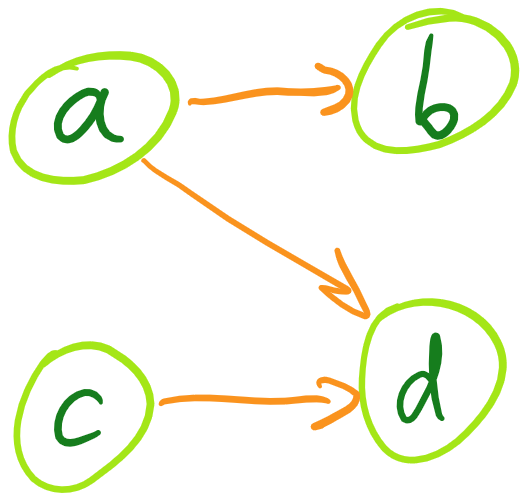
\includegraphics[scale=0.17]{images/graph_0_01.png}
		\pitem $V := \{a, b, c, d\}, E := \{(a,a), (b,b), (c,c)\}$\\
		\p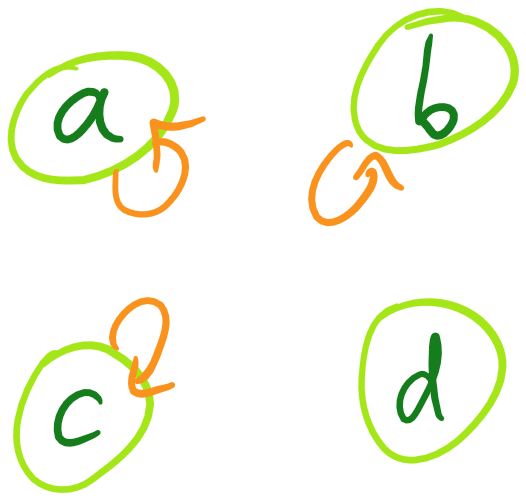
\includegraphics[scale=0.17]{images/graph_0_02.png}
		\pitem $V := \{a, b, c, d\}, E := \emptyset$\\
		\p
\includegraphics[scale=0.17]{images/graph_0_03.png}
	\end{itemize}
\end{frame}

\begin{frame}{Wann Angabe als Menge, wann als Visualisierung?}
	Wir verwenden gezeichnete Graphen und deren Definition als Mengen als äquivalent.
	
	\begin{itemize}
		\pitem $\{(a,b),(c,d),(a,d)\} = \{(a,b),(a,d),(c,d)\} \neq \{(b,a),(d,c),(d,a)\}$, also Kantenmenge mit unterschiedlichen Reihenfolgen darstellbar. Genauso die Knotenmenge.
	\end{itemize}

	\ip
	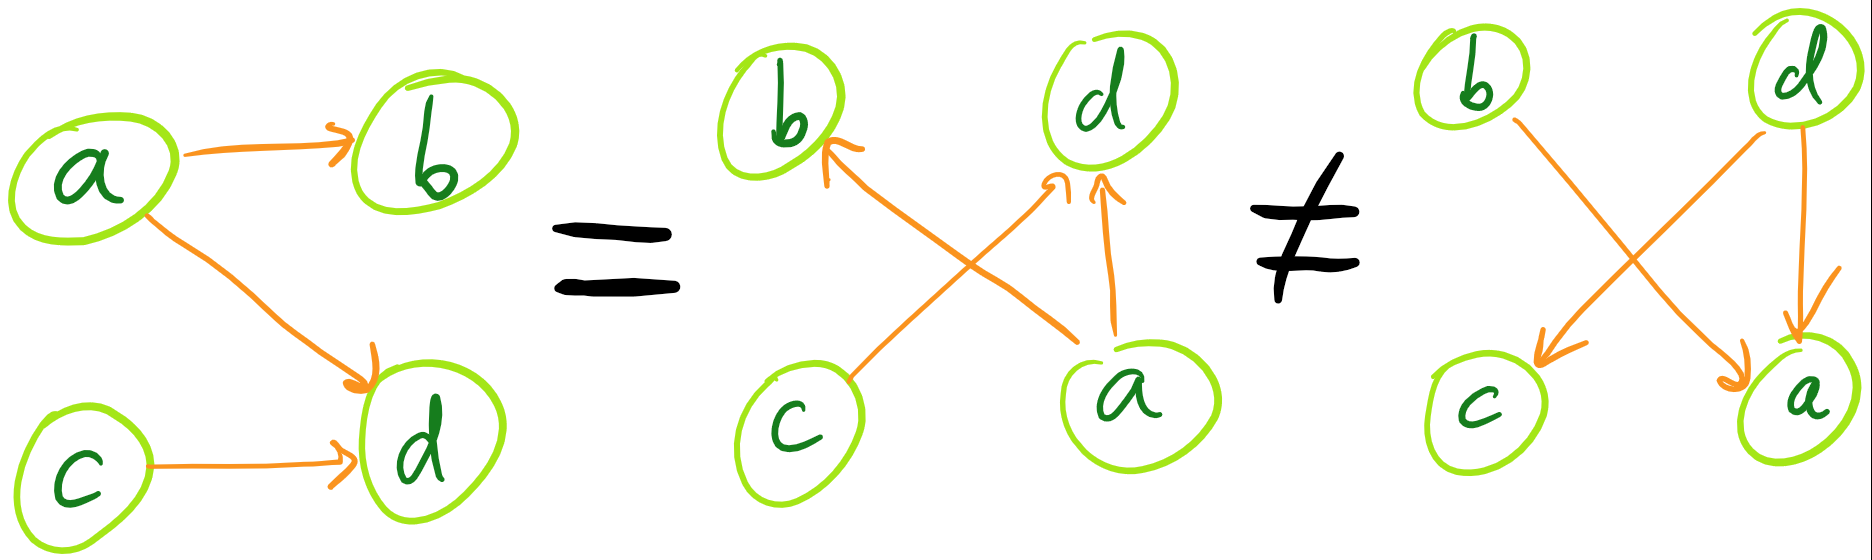
\includegraphics[scale=.3]{images/graph_1.png}
	
	\bp
	
	Es kann also in jedem Fall der Graph sowohl als ``Visualisierung'' oder als Menge angegeben werden, beide Varianten sind formal korrekt.
\end{frame}

\subsection{Praxisbeispiele}
% Hier bei allen Aussagen fragen, was die Tutanden als Ideen haben, wie man das als Graphenfrage formulieren kann
% Einige Sachen werden vorgegriffen (Wurzel, Knotengrad). Trotzdem fragen, Tutanden werden es vermutlich einfach komplizierter formulieren. Das so stehen lassen und erwähnen, dass darauf später genauer eingegangen wird.
% Dabei soll deutlich werden, dass konkrete Probleme in "die Sprache der Graphen" überführt werden kann und als bekanntes Problem gelöst werden kann

\begin{frame}{Praxisbeispiel: Soziales Netzwerk}
	\ip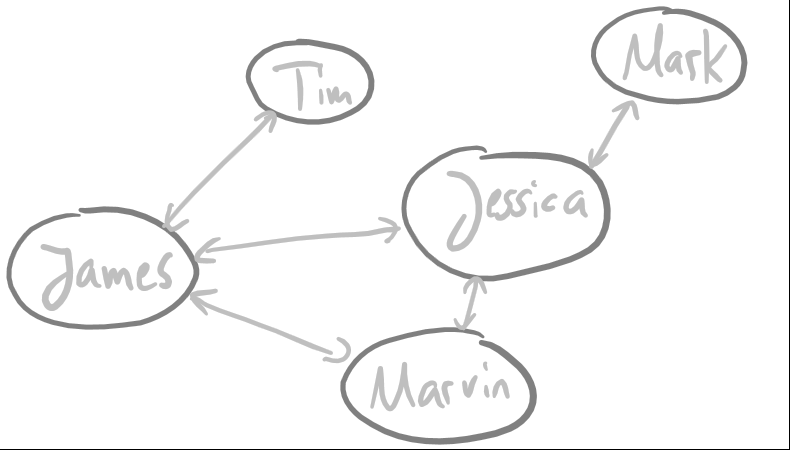
\includegraphics[scale=0.4]{images/graph_beispiel_socialnetwork.png}
	\begin{itemize}
		\pitem Ist Person $A$ direkt mit Person $B$ befreundet? \pause $\Leftrightarrow$ Gibt es eine Kante $(A,B)$?
		\pitem Ist Person $A$ über maximal 2 verschiedene Leute mit Person $B$ befreundet?\pause $\Leftrightarrow$  Gibt es einen Pfad von $A$ nach $B$ mit maximaler Länge 3?
		\pitem Wieviele Freunde hat Person $A$?\pause $\Leftrightarrow$ Welchen Grad hat Person $A \in V$?
	\end{itemize}
\end{frame}

\begin{frame}{Praxisbeispiel: Wie kommt man am schnellsten von $A$ nach $B$}
	\ip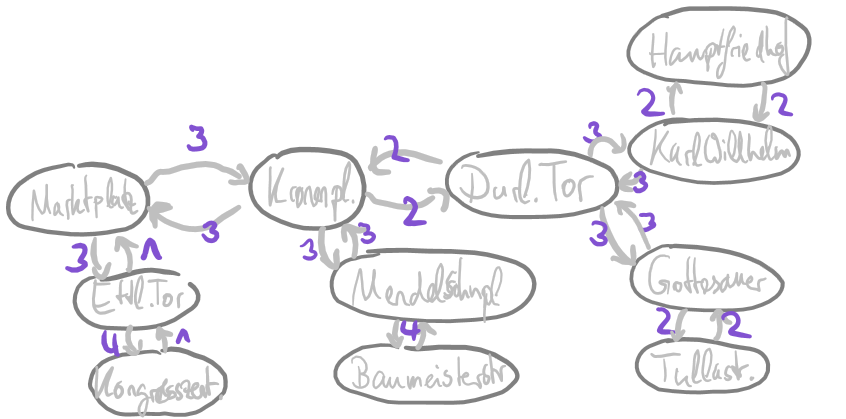
\includegraphics[scale=0.4]{images/graph_beispiel_kvv.png}
	\begin{itemize}
		\pitem Kantengewichtung: Jeder Kante wird eine Zahl $c \in \R$ zugewiesen.
		\pitem Wie lange dauert der kürzeste Weg von Kongresszentrum nach Hauptfriedhof? \pause $\Leftrightarrow$ Wie lang ist ein kürzester Pfad von Kongresszentrum nach Hauptfriedhof?
		\pitem Wo kommt man von Kronenplatz überall innerhalb von 5 Zeiteinheiten hin? \pause $\Leftrightarrow$ Für welche Orte $v \in V$ existiert ein Pfad $(Kronenplatz, ..., v)$ mit einer Länge von maximal 5?
	\end{itemize}
\end{frame}

\begin{frame}{Praxisbeispiel: Huffman-Bäume}
	\ip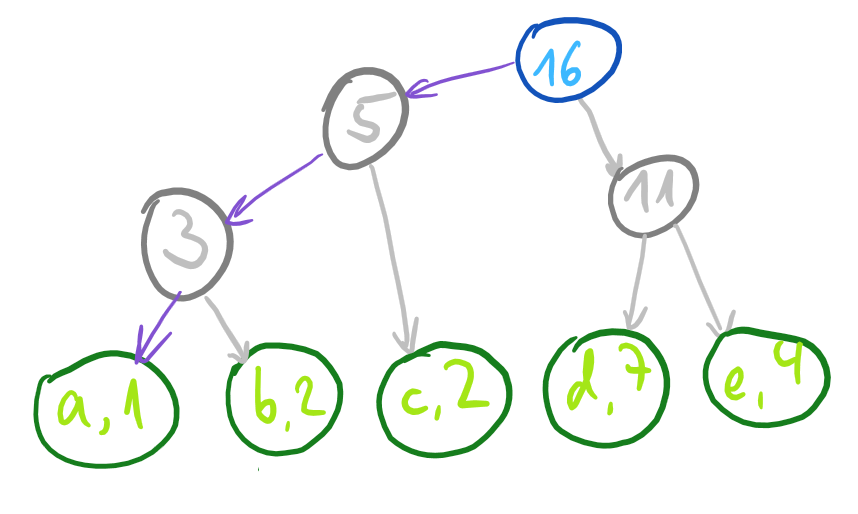
\includegraphics[scale=0.4]{images/graph_beispiel_huffman.png}
	\begin{itemize}
		\pitem Wie lang ist die Kodierung vom Zeichen $c$?\pause $\Leftrightarrow$ Wie lang ist der Pfad von Wurzel zu Knoten $c$? In diesem Fall $2$.
		\pitem Wie viele Zeichen werden kodiert? \pause $\Leftrightarrow$ Wie viele Knoten sind von der Wurzel erreichbar, die selbst keine ausgehenden Kanten haben? \pause $\Leftrightarrow$ Wie viele Blätter hat der Baum?
	\end{itemize}
\end{frame}


\subsection{Ungerichtete Graphen}
\begin{frame}{Ungerichtete Graphen}
	\begin{itemize}
		\pitem Bis jetzt\ip: Gerichtete Graphen\ip, dh. Kanten $(u,v)$ hatten eine Richtung von Knoten $u$ nach Knoten $v$.
	\end{itemize}

	\bp
	
	\begin{block}{Ungerichteter Graph}
		Ein ungerichteter Graph ist ein Graph\ip, dessen Kanten Mengen, und keine Tupel sind.
	\end{block}

	\bp
	
	\begin{itemize}
		\item Beispiel: Statt Kante $(u,v)$ jetzt Kante $\{u,v\} \pause = \{v, u\}$.
		\pitem Information über Richtung geht also verloren, Kanten verbinden nur noch Knoten, ohne sich zu merken, welcher Knoten Start und welcher Ziel ist.
	\end{itemize}
\end{frame}

\subsection{Begriffe}

\begin{frame}{Teilgraph}
	\begin{block}{Teilgraph}
		\ip Zu einem Graph $G := (V, E)$ \ip ist ein Teilgraph definiert \ip als $G' = (V', E')$\ip, falls gilt $V' \subseteq V$ und $E' \subseteq E$.
	\end{block}

	\bp	

	\begin{itemize}
		\item Beispiel: Sei $G := (V,E)$ mit $V := \{a,b,c,d,e,f\}$ und $E := \{(b,a),(b,f),(f,d),(e,f),(f,a),(e,b),(a,e),(f,c),(a,c),(c,a),(c,e)\}$
		\p\item Ist ein Graph mit $V_1:=\{a,c,d,e,f\}, E_1:= \{(a,c),(c,a),(a,e),(f,d)\}$ ein Teilgraph von $G$?
		\p\item Ist ein Graph mit $V_2:=\{d,f\}, E_2:= \{(f,d)\}$ ein Teilgraph von $G$?
		\p\item Ist ein Graph mit $V_3=E_3=\emptyset$ ein Teilgraph von $G$?
	\end{itemize}

	\bp
	
	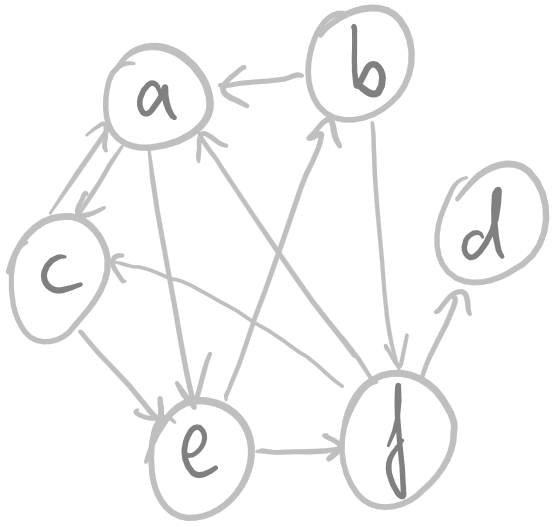
\includegraphics[scale=0.2]{images/graph_teilgraph_01.png}\ip
	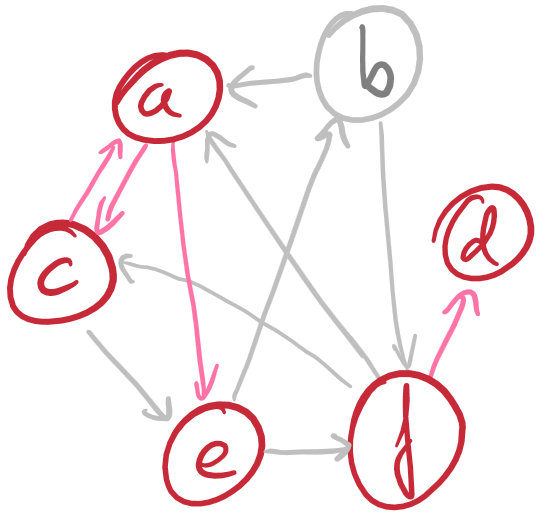
\includegraphics[scale=0.2]{images/graph_teilgraph_02.png}\ip
	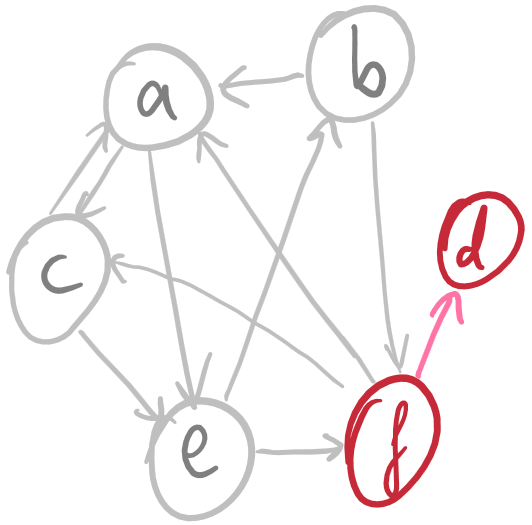
\includegraphics[scale=0.2]{images/graph_teilgraph_03.png}\ip
	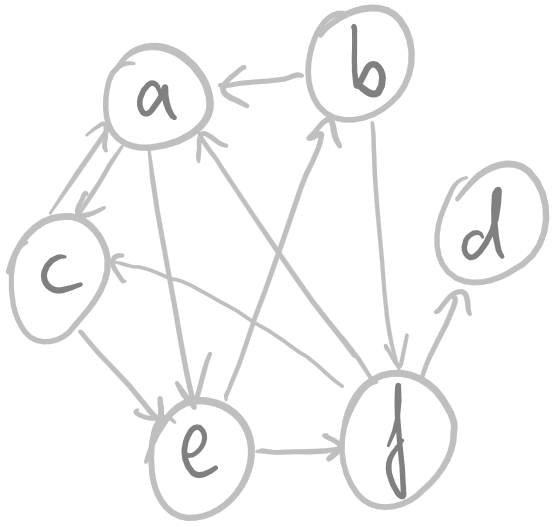
\includegraphics[scale=0.2]{images/graph_teilgraph_01.png} % Das ist technisch noch der letzte graph mit leeren kanten/knoten mengen
\end{frame}

\begin{frame}{Teilgraph}
	\begin{block}{Teilgraph}
		Zu einem Graph $G := (V, E)$ ist ein Teilgraph definiert als $G' = (V', E')$, falls gilt $V' \subseteq V$ und $E' \subseteq E$.
	\end{block}
	
	\begin{itemize}
		\item Beispiel: Sei $G := (V,E)$ mit $V := \{a,b,c,d,e,f\}$ und $E := \{(b,a),(b,f),(f,d),(e,f),(f,a),(e,b),(a,e),(f,c),(a,c),(c,a),(c,e)\}$
		\p\item Ist ein Graph mit $V_4:=\{a,b\}, E_4:= \{(f,d)\}$ ein Teilgraph von $G$?
		\p\item Ist ein Graph mit $V_5:=\{g,a\}, E_5:=\{(g,a),(a,g)\}$ ein Teilgraph von $G$?
		% Beides nicht.
	\end{itemize}
\end{frame}

\begin{frame}{Weg/Pfad}
	\begin{columns}
		\begin{column}{0.6\textwidth}
			\begin{block}{Pfad informell}
				Ein Pfad $(u,...,v)$ ist eine Aneinanderreihung von Knoten\ip, die jeweils mit Kanten verbunden sind\ip, sodass man über das \markGreen{traversieren} der Kanten vom Startknoten $u\in V$ zum Zielknoten $v\in V$ kommt.
			\end{block}
			
			\bp
			Anmerkung: Wenn man sich einen Knoten $x \in V$ merkt und eine Kante $(x,y) \in E$ traversiert, so gelangt man zu Knoten $y$.
			\bp
			
			\begin{block}{Pfad formell}
				Ein Pfad $P := (v_0, v_1, ..., v_n)$ der Länge $n$ \ip ist eine Permutation auf $V$ \ip, wobei gilt: \ip $\forall i \in \Z_n: (v_i, v_{i+1}) \in E$.
			\end{block}	
		\end{column}
		
		\begin{column}{0.4\textwidth}
			\bp
			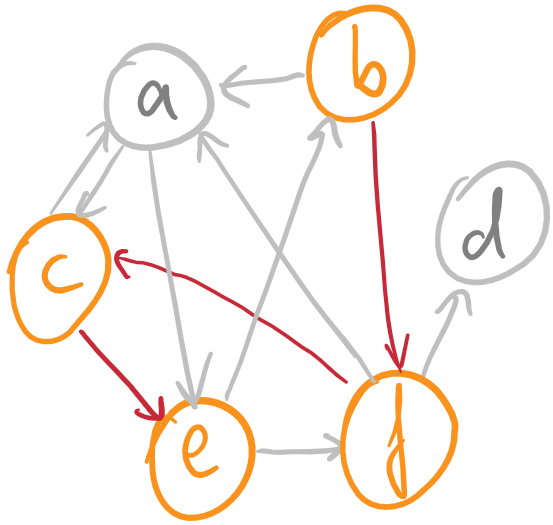
\includegraphics[scale=0.3]{images/graph_pfad.png}
			
			\ip Der Pfad $(b,f,c,e)$ ist ein möglicher Pfad von $b$ nach $e$ der Länge 3.
			
			\ip Gibt es noch andere solcher Pfade?
		\end{column}
	\end{columns}
\end{frame}

\begin{frame}{Zyklus}
	\begin{block}{Zyklus}
		\ip Ein Zyklus ist ein Pfad $(v_1, ..., v_n)$ mit $v_1 = v_n$.
	\end{block}
	\bp
	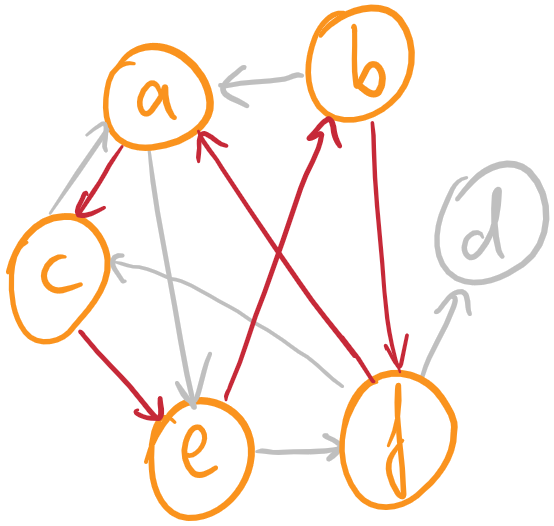
\includegraphics[scale=0.3]{images/graph_zyklus.png}
	
	\ip Der Pfad $(b,f,a,c,e)$ ist ein möglicher Zyklus.
	
	\ip Gibt es noch andere Zyklen?
\end{frame}

\begin{frame}{Zusammenhängend}

	% Jeweils Beispiele an der Tafel vormalen.

	\bp
	
	\begin{block}{Zusammenhängender Graph}
		Ein ungerichteter Graph heißt zusammenhängend, wenn gilt: $\forall u,v \in V \exists$ Pfad von $u$ nach $v$.
	\end{block}

	\bp

	\begin{block}{Stark zusammenhängender Graph}
		Ein gerichteter Graph heißt stark zusammenhängend, wenn gilt: $\forall u,v \in V \exists$ Pfad von $u$ nach $v$.
	\end{block}

	\bp
	
	\begin{block}{Schwach zusammenhängender Graph}
	Ein gerichteter Graph heißt schwach zusammenhängend, wenn der zugehörige ungerichteter Graph zusammenhängend ist.
	\end{block}
\end{frame}

\begin{frame}{Knotengrad}
	
	% Jeweils Beispiele an der Tafel vormalen.
	
	\begin{block}{Eingangsgrad}
		Der Eingangsgrad eines Knoten $u \in V$ ist definiert als: $d_{-}(u) := |\{(v, u) \in E: v \in V\}|$\ip, also die Anzahl der Kanten, die in den Knoten $u$ zeigen.
	\end{block}

	\bp 

	\begin{block}{Ausgangsgrad}
	Der Ausgangsgrad eines Knoten $u \in V$ ist definiert als: $d_{+}(u) := |\{(u, v) \in E: v \in V\}|$\ip, also die Anzahl der Kanten, die vom Knoten $u$ aus weg zeigen.
	\end{block}

	\bp
	
	\begin{block}{Grad}
		Der Grad eines Knoten $u$ ist definiert als: $d(u) := d_{+}(u) + d_{-}(u)$\ip, also die Anzahl der Kanten, über die $u$ verbunden ist.
	\end{block}
\end{frame}

\begin{frame}{Gerichtete Bäume}
	
	% Jeweils Beispiele an der Tafel vormalen.
	
	\begin{itemize}
		\pitem Kennt ihr schon: Huffman-Baum
	\end{itemize}

	\begin{block}{Gerichteter Baum}
	Ein gerichteter Baum ist ein \markGreen{schwach zusammenhängender kreisfreier} gerichteter Graph.	
	\end{block}

	\bp

	\begin{block}{Ungerichteter Baum}
		Ein ungerichteter Baum ist ein \markGreen{zusammenhängender kreisfreier} ungerichteter Graph.	
	\end{block}

	\bp

	\begin{itemize}
		\pitem Bäume haben immer einen Wurzelknoten, von dem alle anderen Knoten ausgehen.
		\pitem Ungerichtete Bäume \markBlue{können} mehrere Wurzeln haben.
		\pitem Knoten mit Grad 1 heißen Blätter.
	\end{itemize} 
\end{frame}



\begin{frame}{Randfälle}
	\begin{itemize}
		\pitem Wieviele Kanten kann ein Graph mit $n$ Knoten maximal haben? \pause $n^2$
		\pitem Wieviele Kanten kann ein schlingenfreier Graph mit $n$ Knoten maximal haben? \pause $n^2-n \p = n(n-1)$
		\pitem Wieviele Kanten kann ein ungerichteter Graph mit $n$ Knoten maximal haben? \pause $\frac{n(n-1)}{2} + n\p = \frac{n(n+1)}{2}$
		\pitem Wieviele Kanten kann ein ungerichteter schlingenfreier Graph mit $n$ Knoten maximal haben? \pause $\frac{n(n-1)}{2}$
	\end{itemize}
\end{frame}

\ifdefined\compileall
\else


\ifthenelse{\equal{\compiletype}{print}}
{

\begin{frame}{Informationen}
	
	\begin{columns}
		\begin{column}{0.5\textwidth}
			
			\begin{block}{Zum Tutorium}
				\begin{itemize}
					\item Lukas Bach
					\item Tutorienfolien auf: 
					\begin{itemize}
						\item \url{http://gbi.lukasbach.com}
					\end{itemize}
					\item Tutorium findet statt:
					\begin{itemize}
						\item Donnerstags, 14:00 - 15:30
						\item 50.34 Informatikbau, -107
					\end{itemize}
				\end{itemize}
			\end{block}
			
			\begin{block}{Mehr Material}
				\begin{itemize}
					\item Ehemalige GBI Webseite:
					\begin{itemize}
						\item \url{http://gbi.ira.uka.de}
						\item Altklausuren!
					\end{itemize}
				\end{itemize}
			\end{block}
			
		\end{column}
		\begin{column}{0.5\textwidth}
			
			\begin{block}{Zur Veranstaltung}
				\begin{itemize}
					\item Grundbegriffe der Informatik
					\item Klausurtermin:
					\begin{itemize}
						\item 06.03.2017, 11:00
						\item Zwei Stunden Bearbeitungszeit
						\item 6 ECTS für Informatiker und Informationswirte, 4 ECTS für Mathematiker und Physiker
					\end{itemize}
				\end{itemize}
			\end{block}
			
			\begin{block}{Zum Übungsschein}
				\begin{itemize}
					\item Übungsblatt jede Woche
					\item Ab 50\% insgesamt hat man den Übungsschein
					\item Keine Voraussetzung für die Klausur, aber für das Modul
				\end{itemize}
			\end{block}
			
		\end{column}
	\end{columns}
	
\end{frame}

}{}

\ifdefined\livebeamermode
	\begin{frame}
		
\includegraphics[width=\linewidth]{images/thatsall.png}
	\end{frame}
\fi

\end{document}

\fi
\def\tutdate{19.01.2017}
\ifdefined\compileall \else
\ifdefined\compiletype
	\documentclass[handout]{beamer}
\else
	\documentclass{beamer}
	\def\compiletype{livebeamer}
\fi

\usepackage{templates/beamerthemekitwide}

\usepackage[utf8]{inputenc}
\usepackage[T1]{fontenc}
\usepackage[ngerman]{babel}
\usepackage{listings}
\usepackage{hyperref}
\usepackage{graphicx}

\usepackage{amsmath}
\usepackage{amsthm}
\usepackage{amssymb}
\usepackage{polynom}

\usepackage{ifthen}
\usepackage{adjustbox} % for \adjincludegraphics

\newcommand{\markBlue}[1]{\textcolor{kit-blue100}{#1}}
\newcommand{\markGreen}[1]{\textcolor{kit-green100}{#1}}

\newcommand{\pitem}{\pause\item}
\newcommand{\p}{\pause}

% -- MATH MACROS
\newcommand{\thistheoremname}{}
\newcommand{\G}{\mathbb{Z}}
\newcommand{\B}{\mathbb{B}}
\newcommand{\R}{\mathbb{R}}
\newcommand{\N}{\mathbb{N}}
\newcommand{\Q}{\mathbb{Q}}
\newcommand{\C}{\mathbb{C}}
\newcommand{\Z}{\mathbb{Z}}
\newcommand{\F}{\mathbb{F}}
\newcommand{\mi}{\mathrm{i}}
\renewcommand{\epsilon}{\varepsilon}


\newenvironment<>{taskblock}[1]{%
	\setbeamercolor{block title}{fg=kit-orange15,bg=kit-orange100}
	\setbeamercolor{block body}{fg=black,bg=kit-orange30}%
	\begin{block}#2{#1}}{\end{block}}

\setbeamertemplate{enumerate items}[default]

% Aussagenlogik Symbole
\newcommand{\W}{w}
\renewcommand{\F}{f}

% Kodierung
\newcommand{\frepr}{\textbf{repr}}
\newcommand{\fRepr}{\textbf{Repr}}
\newcommand{\fZkpl}{\textbf{Zkpl}}
\newcommand{\fbin}{\textbf{bin}}
\newcommand{\fdiv}{\textbf{ div }}
\newcommand{\fmod}{\textbf{ mod }}

\title[Grundbegriffe der Informatik]{Grundbegriffe der Informatik\\Tutorium 33}
\subtitle{}
\author{Lukas Bach, lukas.bach@student.kit.edu}
\date{\tutdate}

\institute{}

\titlelogo{lukasbach}

\titleimage{bg}
%\titleimage{bg-advent}


\ifthenelse{\equal{\compiletype}{livebeamer}}
	{
		\def\livebeamermode{1}
	}{}

\ifthenelse{\equal{\compiletype}{print}}
	{
		\def\printmode{1}
	}{}

\setbeamercovered{invisible}

%\usepackage[citestyle=authoryear,bibstyle=numeric,hyperref,backend=biber]{biblatex}
%\addbibresource{templates/example.bib}
%\bibhang1em

\begin{document}
	
\selectlanguage{ngerman}


%title page
\begin{frame}
	\titlepage
\end{frame}

%table of contents
\ifdefined\printmode
	\ifdefined\compileall \else
	\begin{frame}{Gliederung}
		\tableofcontents
	\end{frame}
\fi\fi

\fi

\section{Repräsentation von Graphen}
\begin{frame}{Repräsentation von Graphen}
	Wie stellen wir Graphen da?\\\ip
	\center{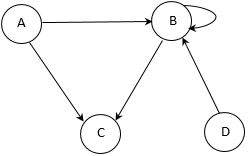
\includegraphics[scale=0.6]{images/Graph1.png}}\\
	Anschaulich ja, aber wie können wir Graphen z.B. mit Java realisieren?
\end{frame}

%Selber drauf kommen lassen
\begin{frame}{Objektorientierte Repräsentation von Graphen}
	Klassenmodell?\pause
	
	\begin{alltt}
		class Vertex \{ 					\\                                  
		\hspace{0.4cm} String name; //Genauer Inhalt interessiert uns nicht	\\                               
		\}   
		\vspace{0.3cm}        			\\               
		class Edge \{ 					\\ 
		\hspace{0.4cm}	Vertex start;    \\
		\hspace{0.4cm}	Vertex end;     \\
		\}  
		\vspace{0.3cm}                    \\               
		class Graph \{					\\
		\hspace{0.4cm}   Vertex[] vertices;\\
		\hspace{0.4cm}   Edge[] edges;	\\
		\}								\\
	\end{alltt}
\end{frame}

\begin{frame}{Objektorientierte Repräsentation von Graphen}
	\begin{itemize}
		\pitem[\textbf{+}] Intuitiv
		\pitem[\textbf{--}] Es lassen sich nur schwer Algorithmen hierfür entwerfen (z.B. gilt $(x,y) \in E$?)
	\end{itemize}
\end{frame}

\subsection{Adjazenzlisten}
\begin{frame}{Repräsentation mit Adjazenzlisten}
	Jeder Knoten speichert seine Nachbarn:
	\begin{alltt}
		class Vertex \{ 					\\                                  
		\hspace{0.4cm} String name; //Genauer Inhalt interessiert uns nicht	\\                               
		\hspace{0.4cm}   \textcolor{blue}{Vertex[] neighbours;} //Alle Nachbarknoten\\
		\}\\
		\vspace{0.3cm}
		class Graph \{					\\
		\hspace{0.4cm}   Vertex[] vertices;\\
		\hspace{0.4cm}  \deleted{Edge[] edges;}	\\
		\}	\\
	\end{alltt}
\end{frame}

\begin{frame}{Repräsentation mit Adjazenzlisten}
	\begin{itemize}
		\item[\textbf{+}] Speicherplatzeffizient bei wenigen Kanten im Vergleich zur Knotenanzahl ($|E| << |V|^2$)
		\item[\textbf{+}] Flexibel mit verketteten Listen statt Arrays (Leichtes Hinzufügen und Entfernen)
	\end{itemize}
\end{frame}



\begin{frame}{Repräsentation mit Adjazenzmatrix}
	\begin{itemize}
		\pitem Was ist eine Adjazenzmatrix?
		\pitem Zu allen Paaren $(i,j) \text{ mit } i, j \in V$ wird gespeichert, ob $(i,j) \in E$ gilt
		\pitem Zweidimensionales Array
	\end{itemize}
	\begin{alltt}
		class Graph \{					\\
		\hspace{0.4cm}   boolean[][] edges; //Größe $|V| \times |V|$\\
		\}	\\
	\end{alltt}
\end{frame}

\begin{frame}{Repräsentation mit Adjazenzmatrix}
	\begin{itemize}
		\pitem[\textbf{+}] Speicherplatzeffizient bei annähernd maximaler Anzahl von Kanten ($|E| \approx |V|^2$)
		\pitem[+] Algorithmen aus linearer Algebra können verwendet werden (Matrizenrechnung)
		\pitem[\textbf{--}] nicht flexibel
	\end{itemize}
\end{frame}

\begin{frame}
	\textbf{Aufgabe}\\
	Gebe alle Adjazenlisten und die Adjazenzmatrix für diesen Graphen an:
	\center{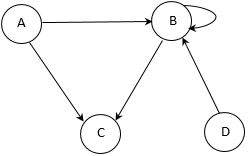
\includegraphics[scale=0.6]{images/Graph1.png}}
	\pause
	$ A =
	\begin{pmatrix}
	0&1&1&0\\
	0&1&1&0\\
	0&0&0&0\\
	0&1&0&0\\
	\end{pmatrix}	
	$
\end{frame}

\begin{frame}{Repräsentation von zweistelligen Relationen durch Matrizen}
	Wir können jede endliche zweistellige Relation durch eine Matrix darstellen!\\
	\textbf{Aufgabe}\\
	Stelle die Kleiner-Gleich-Relation auf der Menge $\{0, 1, 2, 3\}$ dar!\\
	\pause
	$ R_{\leq} =
	\begin{pmatrix}
	1&1&1&1\\
	0&1&1&1\\
	0&0&1&1\\
	0&0&0&1\\
	\end{pmatrix}	
	$
\end{frame}

\section{Erreichbarkeit}
\begin{frame}{Wege-Problem}
	\begin{itemize}
		\pitem Algorithmisches Problem
		\pitem Intuitiv: Gibt es einen Weg von $i$ nach $j$?
	\end{itemize}

	\pause
	
	\begin{block}{Wege-Problem}
		Gegeben einem Graphen $G = (V,E)$. Ist für $i,j \in V$ auch $(i,j) \in E^*$?
	\end{block}

	\pause

	\textbf{Ziel}\\
	\begin{itemize}
		\pitem Gegeben: Adjazenzmatrix
		\pitem Gesucht: Zugehörige \textbf{Wegematrix}, für die gilt:
	\end{itemize}

	\pause

	$W_{ij} = \begin{cases} 
	1 & \text{, falls ein Weg von i nach j existiert}\\
	0 & \text{, sonst}
	\end{cases}$
\end{frame}

\begin{frame}{Einschub Matrizen}
	Was wisst ihr zu folgenden Begriffen?
	
	\begin{itemize}
		\pitem Matrizenmultiplikation
		\pitem Matrizenaddition
		\pitem Potenzieren
		\pitem Einheitsmatrix
		\pitem Nullmatrix
	\end{itemize}
\end{frame}

\begin{frame}{Quadrierte Adjazenzmatrix}
	\textbf{Aufgabe}\\
	Quadriere die Adjazenzmatrix von vorhin:
	$ A =
	\begin{pmatrix}
	0&1&1&0\\
	0&1&1&0\\
	0&0&0&0\\
	0&1&0&0\\
	\end{pmatrix}	
	$
	\pause 
	
	\textbf{Ergebnis}\\
	$ A^2 =
	\begin{pmatrix}
	0&1&1&0\\
	0&1&1&0\\
	0&0&0&0\\
	0&1&1&0\\
	\end{pmatrix}	
	$
\end{frame}

\begin{frame}
	\textbf{Aufgabe}\\
	Bilde und quadriere die Adjazenzmatrix des veränderten Graphen:\\
	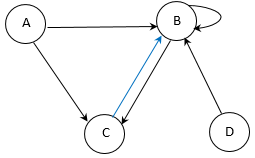
\includegraphics[scale=0.6]{images/Graph2_edit.png}\\
	\pause
	$ A' =
	\begin{pmatrix}
	0&1&1&0\\
	0&1&1&0\\
	0&1&0&0\\
	0&1&0&0\\
	\end{pmatrix}	
	$ 
	und 
	$ A'^2 =
	\begin{pmatrix}
	0&2&1&0\\
	0&2&1&0\\
	0&1&1&0\\
	0&1&1&0\\
	\end{pmatrix}	
	$
\end{frame}

\begin{frame}
	\textbf{Aufgabe}\\
	Was fällt euch auf? Wann steht in $A'^2$ eine $1$, wann eine $2$ und was bedeutet das für unseren Graphen?\\
	$ A' =
	\begin{pmatrix}
	0&1&1&0\\
	0&1&1&0\\
	0&1&0&0\\
	0&1&0&0\\
	\end{pmatrix}	
	$ 
	$ A'^2 =
	\begin{pmatrix}
	0&2&1&0\\
	0&2&1&0\\
	0&1&1&0\\
	0&1&1&0\\
	\end{pmatrix}	
	$ 
	\pause
	\includegraphics[scale=0.6]{images/Graph2.png} \hspace{0.3cm}\pause
	\includegraphics[scale=0.5]{images/multiplikation.png}\\
	\textbf{Tipp:} $c_{11} = a_{11} \cdot b_{11} + a_{12} \cdot b_{21} + a_{13} \cdot b_{31}$
\end{frame}

\begin{frame}
	\textbf{Lösung}\\
	In der $i$-ten Zeile und $j$-ten Spalte von $A^2$ steht die Anzahl der Wege von $i$ nach $j$ der Länge zwei.\\
	\begin{itemize}
		\item[$\rightarrow$]$(A^2)_{ij}$ = Anzahl der Pfade von $i$ nach $j$ der Länge zwei.
	\end{itemize}

	\pause

	\textbf{Aufgabe}\\
	Habt ihr Ideen, wie man herausfindet, zwischen welchen Knoten Pfade der Länge $n$ existieren?\\
	\pause
	\textbf{Lösung}\\
	Betrachte $A^n$!
\end{frame}

\subsection{Zwei-Erreichbarkeit}
\begin{frame}{Zwei-Erreichbarkeit}
	Eigentlich interessiert uns nur, ob ein Pfad der Länge zwei existiert und nicht wie viele...
	\pause
	\begin{block}{Definition Signum-Funktion}
		$sgn: \mathbb{R}\rightarrow \mathbb{R}$\\
		$x \mapsto \begin{cases}
		1& \text{, falls } x > 0\\
		0 & \text{, falls } x = 0\\
		-1& \text{, falls } x < 0
		\end{cases}$
	\end{block}
	\pause
	$sgn(A^2)$ liefert uns die Zwei-Erreichbarkeitsmatrix
\end{frame}

\subsection{Erreichbarkeit}
\begin{frame}
	\textbf{Aufgabe}\\
	Gebe $A^0$, $A^2$ und die Wegematrix $W$ an!
	\includegraphics[scale=0.6]{images/Graph3.png}\\
	\pause
	$ A^0 =
	\begin{pmatrix}
	1&0&0&0\\
	0&1&0&0\\
	0&0&1&0\\
	0&0&0&1\\
	\end{pmatrix}	
	$ \pause
	$ A^2 =
	\begin{pmatrix}
	0&0&1&0\\
	0&0&1&1\\
	0&0&1&1\\
	0&0&0&0\\
	\end{pmatrix}	
	$ \pause
	$ W =
	\begin{pmatrix}
	1&1&1&1\\
	0&1&1&1\\
	0&0&1&1\\
	0&0&0&1\\
	\end{pmatrix}	
	$ 
	
\end{frame}

\begin{frame}{Erreichbarkeit}
	Für Pfade beliebiger Länge erhalten wir:
	$W = sgn(A^0 + A^1 + A^2 + A^3 + ...) = sgn(\sum\limits_{i=0}^{\infty} A^i)$\\
	\pause
	Wir können nicht unendlich lange addieren... Ist das ein \textbf{Problem}? 
\end{frame}

\begin{frame}{Erreichbarkeit- unendlich addieren?}
	\ip Wenn ein Pfad $p$ der Länge $ \geq n := |V|$ zwischen $i \neq j$ existiert, muss mindestens ein Knoten doppelt vorgekommen sein! \ip Der Pfad $p$ enthält also einen Zyklus, den wir raus kürzen können.\\\p
	\vspace{0.15cm}
	\textbf{Ergebnis}\\
	Wenn ein Pfad $p$ der Länge $\geq n := |V|$ zwischen $i \neq j$ existiert, existiert auch ein Pfad $p'$ der Länge $< n$.\\\p
	\vspace{0.4cm}
	Für Pfade beliebiger Länge erhalten wir:
	$W = sgn(A^0 + A^1 + A^2 + A^3 + ...) = sgn(\sum\limits_{i=0}^{\infty} A^i)$ \markBlue{$= sgn (\sum\limits_{i=0}^{n-1} A^i)$} \\
\end{frame}

\subsection{Algorithmus}
\begin{frame}{Einfacher Algorithmus zu Berechnung der Wegematrix}
	\only<1>{\includegraphics[scale=0.7]{images/algo1.png}}
	\only<2,3>{\includegraphics[scale=0.7]{images/algo1_bed.png} \includegraphics[scale=0.8]{images/aufwand.png} }
	\only<3>{\\ Wie könnte man diesen Algorithmus schneller machen?}
	\only<4>{\includegraphics[scale=0.8]{images/algo2.png}}
\end{frame}
\section{Komplexitätstheorie}

\begin{frame}{Komplexitätstheorie}
	\pause
	Wichtige Komplexitätsmaße:
	\begin{itemize}
		\pitem Speicherplatzbedarf
		\pitem Rechen- bzw. Laufzeit
	\end{itemize}
	Unterscheidung in
	\begin{itemize}
		\pitem Best Case (oft uninteressant)
		\pitem Average Case (schwierig zu finden, deswegen selten angegeben)
		\pitem Worst Case  (meistens angegeben)
	\end{itemize}
\end{frame} 

\subsection{O-Notation}
\begin{frame}{Ignorieren konstanter Faktoren}
	\begin{block}{Definition}
		Seien $g,f: \mathbb{N}_0 \rightarrow \mathbb{R}_0^+$ Funktionen. Dann wächst $g$ asymptotisch genauso schnell wie $f$ genau dann, wenn gilt:\\
		$\exists c, c' \in \mathbb{R}_+ : \exists n_0 \in \mathbb{N}_0: \forall n \geq n_0 : c \cdot f(n) \leq g(n)\leq c' \cdot f(n)$
	\end{block}
	\pause

	\textbf{Notation}\\
	$f \asymp g$ oder $f(n) \asymp g(n)$ ("asymptotisch gleich")\\
	\textbf{Bemerkung}\\
	$\asymp$ ist eine Äquivalenzrelation
\end{frame}

\begin{frame}{Theta}
	\begin{block}{Definition}
		$\Theta (f) = \{g|g \asymp f\}$
	\end{block}

	\pause
	
	\begin{block}{Satz}
		$\forall a, b \in \mathbb{R}_+ : \Theta (a\cdot f) = \Theta (b \cdot f)$
	\end{block}
\end{frame}

\begin{frame}{Obere und untere Schranke}
	\begin{block}{Obere Schranke (Worst-Case Approximation)}
		$O(f) = \{g| \exists c \in \mathbb{R}_+ : \exists n_0 \in \mathbb{N}_0: \forall n \geq n_0 : g(n)\leq c \cdot f(n)\}$
	\end{block}

	\pause
	
	\begin{block}{Untere Schranke (Best-Case Approximation)}
		$\Omega(f) = \{g| \exists c \in \mathbb{R}_+ : \exists n_0 \in \mathbb{N}_0: \forall n \geq n_0 : g(n)\geq c \cdot f(n)\}$
	\end{block}
	\pause
	\textbf{Notation}\\
	\begin{itemize}
		\item $g\curlyeqprec f$ falls $g \in O(f)$ bzw. g wächst asymptotisch höchstens so schnell wie f
		\item $g \curlyeqsucc f $ falls $g \in \Omega (f)$ bzw. g wächst asymptotisch mindestens so schnell wie f
	\end{itemize}
	\pause
	\textbf{Bemerkung}\\
	Es gilt $\Theta (f) = O(f) \cap \Omega (f)$
\end{frame}

\begin{frame}
	\begin{block}{Lemma}
		$log_a n \in \Theta (log_b n)$
	\end{block}
	\textbf{Beispiel}\\
	$log_2 n \in \Theta(log_8 n)$\\
	\pause
	\textbf{Beweis}\\
	$\frac{1}{3} log_2 n \ip= \frac{1}{log_2 8} log_2 n \ip= \frac{log_2 n}{log_2 8} \ip= log_8 n \leq log_2 n$
\end{frame}

\begin{frame}
	\textbf{Aufgabe}\\
	Gilt $log_2(n^{20}) \in \Theta (log \space n)$\\
	\pause
	\textbf{Lösung}\\
	Ja, denn $log_2 (n^{20}) = 20 \cdot log_2 n$
\end{frame}

\begin{frame}
	Probeklausur
\end{frame}

\ifdefined\compileall
\else


\ifthenelse{\equal{\compiletype}{print}}
{

\begin{frame}{Informationen}
	
	\begin{columns}
		\begin{column}{0.5\textwidth}
			
			\begin{block}{Zum Tutorium}
				\begin{itemize}
					\item Lukas Bach
					\item Tutorienfolien auf: 
					\begin{itemize}
						\item \url{http://gbi.lukasbach.com}
					\end{itemize}
					\item Tutorium findet statt:
					\begin{itemize}
						\item Donnerstags, 14:00 - 15:30
						\item 50.34 Informatikbau, -107
					\end{itemize}
				\end{itemize}
			\end{block}
			
			\begin{block}{Mehr Material}
				\begin{itemize}
					\item Ehemalige GBI Webseite:
					\begin{itemize}
						\item \url{http://gbi.ira.uka.de}
						\item Altklausuren!
					\end{itemize}
				\end{itemize}
			\end{block}
			
		\end{column}
		\begin{column}{0.5\textwidth}
			
			\begin{block}{Zur Veranstaltung}
				\begin{itemize}
					\item Grundbegriffe der Informatik
					\item Klausurtermin:
					\begin{itemize}
						\item 06.03.2017, 11:00
						\item Zwei Stunden Bearbeitungszeit
						\item 6 ECTS für Informatiker und Informationswirte, 4 ECTS für Mathematiker und Physiker
					\end{itemize}
				\end{itemize}
			\end{block}
			
			\begin{block}{Zum Übungsschein}
				\begin{itemize}
					\item Übungsblatt jede Woche
					\item Ab 50\% insgesamt hat man den Übungsschein
					\item Keine Voraussetzung für die Klausur, aber für das Modul
				\end{itemize}
			\end{block}
			
		\end{column}
	\end{columns}
	
\end{frame}

}{}

\ifdefined\livebeamermode
	\begin{frame}
		\includegraphics[width=\linewidth]{images/thatsall.png}
	\end{frame}
\fi

\end{document}

\fi
\def\tutdate{26.01.2017}
\ifdefined\compileall \else
\ifdefined\compiletype
	\documentclass[handout]{beamer}
\else
	\documentclass{beamer}
	\def\compiletype{livebeamer}
\fi

\usepackage{templates/beamerthemekitwide}

\usepackage[utf8]{inputenc}
\usepackage[T1]{fontenc}
\usepackage[ngerman]{babel}
\usepackage{listings}
\usepackage{hyperref}
\usepackage{graphicx}

\usepackage{amsmath}
\usepackage{amsthm}
\usepackage{amssymb}
\usepackage{polynom}

\usepackage{ifthen}
\usepackage{adjustbox} % for \adjincludegraphics

\newcommand{\markBlue}[1]{\textcolor{kit-blue100}{#1}}
\newcommand{\markGreen}[1]{\textcolor{kit-green100}{#1}}

\newcommand{\pitem}{\pause\item}
\newcommand{\p}{\pause}

% -- MATH MACROS
\newcommand{\thistheoremname}{}
\newcommand{\G}{\mathbb{Z}}
\newcommand{\B}{\mathbb{B}}
\newcommand{\R}{\mathbb{R}}
\newcommand{\N}{\mathbb{N}}
\newcommand{\Q}{\mathbb{Q}}
\newcommand{\C}{\mathbb{C}}
\newcommand{\Z}{\mathbb{Z}}
\newcommand{\F}{\mathbb{F}}
\newcommand{\mi}{\mathrm{i}}
\renewcommand{\epsilon}{\varepsilon}


\newenvironment<>{taskblock}[1]{%
	\setbeamercolor{block title}{fg=kit-orange15,bg=kit-orange100}
	\setbeamercolor{block body}{fg=black,bg=kit-orange30}%
	\begin{block}#2{#1}}{\end{block}}

\setbeamertemplate{enumerate items}[default]

% Aussagenlogik Symbole
\newcommand{\W}{w}
\renewcommand{\F}{f}

% Kodierung
\newcommand{\frepr}{\textbf{repr}}
\newcommand{\fRepr}{\textbf{Repr}}
\newcommand{\fZkpl}{\textbf{Zkpl}}
\newcommand{\fbin}{\textbf{bin}}
\newcommand{\fdiv}{\textbf{ div }}
\newcommand{\fmod}{\textbf{ mod }}

\title[Grundbegriffe der Informatik]{Grundbegriffe der Informatik\\Tutorium 33}
\subtitle{}
\author{Lukas Bach, lukas.bach@student.kit.edu}
\date{\tutdate}

\institute{}

\titlelogo{lukasbach}

\titleimage{bg}
%\titleimage{bg-advent}


\ifthenelse{\equal{\compiletype}{livebeamer}}
	{
		\def\livebeamermode{1}
	}{}

\ifthenelse{\equal{\compiletype}{print}}
	{
		\def\printmode{1}
	}{}

\setbeamercovered{invisible}

%\usepackage[citestyle=authoryear,bibstyle=numeric,hyperref,backend=biber]{biblatex}
%\addbibresource{templates/example.bib}
%\bibhang1em

\begin{document}
	
\selectlanguage{ngerman}


%title page
\begin{frame}
	\titlepage
\end{frame}

%table of contents
\ifdefined\printmode
	\ifdefined\compileall \else
	\begin{frame}{Gliederung}
		\tableofcontents
	\end{frame}
\fi\fi

\fi

\section{Komplexitätstheorie}
\begin{frame}{Rückblick}
	\begin{itemize}
		\pitem Was ist $\Omega(f), \Theta(f), \okalk(f)$?
		\pitem Wieso messen wir nicht einfach Laufzeit in ``Anzahl Operationen''?
		
	\end{itemize}
\end{frame}

\begin{frame}{Obere und untere Schranke}
	\begin{block}{Obere Schranke (Worst-Case Approximation)}
		$O(f) = \{g| \exists c \in \mathbb{R}_+ : \exists n_0 \in \mathbb{N}_0: \forall n \geq n_0 : g(n)\leq c \cdot f(n)\}$
	\end{block}
	
	\pause
	
	\begin{block}{Untere Schranke (Best-Case Approximation)}
		$\Omega(f) = \{g| \exists c \in \mathbb{R}_+ : \exists n_0 \in \mathbb{N}_0: \forall n \geq n_0 : g(n)\geq c \cdot f(n)\}$
	\end{block}

	\pause

	\begin{block}{Average-Case Approximation}
		$\Theta(f) = \{g|\exists c, c' \in \mathbb{R}_+ : \exists n_0 \in \mathbb{N}_0: \forall n \geq n_0 : c \cdot f(n) \leq g(n)\leq c' \cdot f(n)\}$
	\end{block}

	\pause
	
	Auf welche Weise wird hier approximiert? % durch weglassen konstanter faktoren, durch setzen eines n_0, ab dem approximation immer gilt
\end{frame}

\begin{frame}
	Gelten folgende Approximationen?
	
	\begin{itemize}
		\pitem $4n^2 + \pi n + 2 \sqrt{n} \in \Theta(n^2)?$ \pause Ja.
		\pitem $5n^2 + \pi n + 2 \sqrt{n} \in \Theta(n^2)?$ \pause Ja.
		\pitem $4n^{2,1} + \pi n + 2 \sqrt{n} \in \Theta(n^2)?$ \pause Nein.
	\end{itemize}

	\bp Es sind immer nur die höchsten Faktoren interessant!
	
	\begin{itemize}
		\pitem $4n^4 + 3c^6 \in \Theta(n^4)$? \pause Ja\ip, $c$ ist eine Konstante, $3c^6=(3c^6)n^0$ hat eine kleinere Potenz als $n^4$.
		\pitem $\log_{4213}(n) \in \Theta(\log_2(n)$ \pause Ja\ip, die Basis des Logarithmus ist im O-Kalkül egal.
		
		\pitem $n! \in \Theta(n^{\pi e 2000})$ \pause Nein\ip, Fakultät wächst asymptotisch schneller als fast alles andere.
	\end{itemize}
\end{frame}

\begin{frame}
	Gelten folgende Approximationen?
	
	\begin{itemize}
		\pitem $4n^3 + 2n^2 \in \okalk(n^5)$? \pause Ja.
		\pitem $4n^3 + 2n^2 \in \okalk(n^4)$? \pause Ja.
		\pitem $4n^3 + 2n^2 \in \okalk(n^3)$? \pause Ja.
		\pitem $4n^3 + 2n^2 \in \okalk(n^2)$? \pause Nein.
		\pitem $4n^3 + 2n^2 \in \Omega(n^5)$? \pause Nein.
		\pitem $4n^3 + 2n^2 \in \Omega(n^4)$? \pause Nein.
		\pitem $4n^3 + 2n^2 \in \Omega(n^3)$? \pause Ja.
		\pitem $4n^3 + 2n^2 \in \Omega(n^2)$? \pause Ja.
	\end{itemize}
\end{frame}

\begin{frame}{Aufgabe}
	\begin{taskblock}{Übungsaufgabe}
		Entscheide für jede Zelle, ob die Formel der Zeile in der Menge der Spalte liegt.
		
		\begin{center}
			\begin{tabular}{r||c|c|c|c|c|c}%*{2}{>{$}c<{$}}|*{4}{>{$}c<{$}}
				\hline
				& $\okalk(n^3)$ & $\okalk(n)$ & $\Theta(c!)$ & $\Theta(n^\pi)$ & $\Omega(n^6)$ & $\Omega(n!)$ \\\hline\hline
				
				$2n^2 + 4n$ 
					& \visible<2->{$\in$}
					& \visible<3->{$\not\in$}
					& \visible<4->{$\not\in$}
					& \visible<5->{$\not\in$}
					& \visible<6->{$\not\in$}
					& \visible<7->{$\not\in$}
					\\\hline
					
				
				$\pi$
					& \visible<8->{$\in$}
					& \visible<9->{$\in$}
					& \visible<10->{$\in$}
					& \visible<11->{$\not\in$}
					& \visible<12->{$\not\in$}
					& \visible<13->{$\not\in$}
					\\\hline
				
				$\log(n)$
					& \visible<14->{$\in$}
					& \visible<15->{$\in$}
					& \visible<16->{$\not\in$}
					& \visible<17->{$\not\in$}
					& \visible<18->{$\not\in$}
					& \visible<19->{$\not\in$}
					\\\hline
				
				$n\log(n)$
					& \visible<20->{$\in$}
					& \visible<21->{$\not\in$}
					& \visible<22->{$\not\in$}
					& \visible<23->{$\not\in$}
					& \visible<24->{$\not\in$}
					& \visible<25->{$\not\in$}
					\\\hline
				
				$n^\pi$
					& \visible<26->{$\not\in$}
					& \visible<27->{$\not\in$}
					& \visible<28->{$\not\in$}
					& \visible<29->{$\in$}
					& \visible<30->{$\not\in$}
					& \visible<31->{$\not\in$}
					\\\hline
				
				$12n^3+7000n^2$
					& \visible<32->{$\in$}
					& \visible<33->{$\not\in$}
					& \visible<34->{$\not\in$}
					& \visible<35->{$\not\in$}
					& \visible<36->{$\not\in$}
					& \visible<37->{$\not\in$}
					\\\hline
				
				$n^3$
					& \visible<38->{$\in$}
					& \visible<39->{$\not\in$}
					& \visible<40->{$\not\in$}
					& \visible<41->{$\not\in$}
					& \visible<42->{$\not\in$}
					& \visible<43->{$\not\in$}
					\\\hline
				
				$n!$
					& \visible<44->{$\not\in$}
					& \visible<45->{$\not\in$}
					& \visible<46->{$\not\in$}
					& \visible<47->{$\not\in$}
					& \visible<48->{$\in$}
					& \visible<49->{$\in$}
					\\\hline
				
				%\visible<1->{\F} & \visible<1->{\F} & \visible<5->{\F} & \visible<9->{\F} & \visible<17->{\W} & \visible<13->{\F} \\\hline
				
			\end{tabular}
		\end{center}
	\end{taskblock}
\end{frame}


\begin{frame}
	\begin{itemize}
		\pitem $\okalk (n^2) \cap \okalk(n) = \okalk(?)$? \pause $= \okalk(n)$.
		\pitem $\okalk(n^2) \cap \Omega(n^3) = \pause \emptyset$
	\end{itemize}
\end{frame}

\begin{frame}
	\includegraphics[scale=0.5]{images/okalk_algo.png}
	
	\begin{itemize}
		\pitem Wie oft wird die innere Schleife durchlaufen? \pause $n-2i+1$ mal.
		\pitem Wie kommen wir jetzt auf die Gesamtlaufzeit?
		\pitem $\sum\limits_{i=0}^{n/2} (n-2i+1) \ip = \frac{n}{2}n -2\sum\limits_{i=0}^{n/2}i+\frac{n}{2} \ip = \frac{n^2}{2}+\frac{n}{2}-2\frac{\frac{n}{2}\cdot \left(\frac{n}{2}+1\right)}{2} \ip = \frac{n^2}{2}+\frac{n}{2}-\frac{n^2}{4}-\frac{n}{2}\ip = \frac{1}{4}n^2$
		\pitem Kann man das einfacher machen?
	\end{itemize}
\end{frame}


\subsection{Mastertheorem}

\begin{frame}{Mastertheorem}
	\ip
	\begin{block}{Formel für Mastertheorem}
		\ip Rekursive Komplexitätsformeln der Form\\
		
		\vspace{.2cm}
		\ip$\quad T(n) = a \cdot T(\frac{n}{b}) + f(n)$
		\vspace{.2cm}
		
		\ip lassen sich mit dem Mastertheorem Komplexitätsklassen zuordnen.
	\end{block}

	\begin{block}{Auflösung des Mastertheorem}
		\begin{description}
			\item[Fall 1:] Wenn $f \in \okalk(n^{\log_b a -\epsilon})$ für ein
			$\epsilon>0$ ist, dann ist $T\in \Theta(n^{\log_b a})$.
			\item[Fall 2:] Wenn $f \in \Theta(n^{\log_b a})$ ist, dann ist
			$T\in \Theta(n^{\log_b a}\log n)$.
			\item[Fall 3:] Wenn $f \in \okalk(n^{\log_b a +\epsilon})$ für ein
			$\epsilon>0$ ist, und wenn es eine Konstante $d$ gibt mit $0<d<1$, so
			dass für alle hinreichend großen $n$ gilt $af(n/b)\leq d f$, dann
			ist $T\in \Theta(f)$.
		\end{description}
	\end{block}
\end{frame}

\begin{frame}{Aufgaben zum Mastertheorem}
	\begin{itemize}
		\pitem $T(n) := 2 T(\frac{n}{4}) + \sqrt{n}$\pause, also $a=2, b=4, f(n) = \sqrt{n}$\pause, also zweiter Fall des Mastertheorems\pause. $T \in \Theta (\sqrt{n}\log n)$
		\pitem $T(n) := 3 T(\frac{n}{2}) + n\log n$\pause, also $a = 3, b=2, f(n) = n\log n$\pause, also erster Fall des Mastertheorems\pause, $T \in \Theta(n^{\log_2 3})$
		\pitem $T(n) := 4 T(\frac{n}{2}) + n^2\sqrt{n}$\pause, also $a = 4, b=2, f(n) = n^2\sqrt{n}$\pause, also dritter Fall des Mastertheorems\pause, $T \in \Theta(n^2\sqrt{n})$.
	\end{itemize}
\end{frame}

%\subsection{Beweisaufgaben}

%\begin{frame}{Beweisaufgabe zu O-Kalkül}
%	\begin{taskblock}{Beweisaufgabe}
%		Zeige, dass gilt: $3n^3 \not\in \okalk(n^2)$.
%	\end{taskblock}
%
%	\pause
%	
%	Annahme: \ip $3n^3 \in \okalk(n^2)$. 
%	
%	\ip Dann gilt: $\exists c \in \R_+ : \exists n_0 \in \N_0 : \forall n \geq n_0 : \ip c\cdot 3n^3 \leq n^2$.
%	
%	\ip Da der linke Term möglichst klein sein soll\ip, können wir $c < 1$ setzen. \ip Sei $k_0 = \%lceil c \rceil ^{-1} \geq c^{-1}$.
%	
%	\ip Dann: $c \cdot 4k_0^3 = c \cdot k_0 \cdot 3k_0^2 \ip = 3m \cdot k_0^2 \ip \geq k_0^2$ \ip ($m$ durch den Rundungsrest).
%	
%	\ip $m > 1$ und $\forall k \in \N_0, k \geq k_0 : 3k^3 > k^2$.
%\end{frame}


\section{Automaten}

\begin{frame}{Definition eines endlichen Automaten}
	\begin{block}{Endlicher Automat}
		Ein endlicher Automat ist ein Tupel $A = (Z, z_0, X, f, Y, g)$ mit...
		
		\begin{itemize}
			\pitem endliche Zustandsmenge $Z$
			\pitem Anfangszustand $z_0 \in Z$
			\pitem Eingabealphabet $X$
			\pitem Zustandsübergangsfunktion $f: Z \times X \rightarrow Z$
			\pitem Ausgabealphabet $Y$
			\pitem Ausgabefunktion 
			\begin{itemize}
				\pitem Mealy-Automat: $g: Z \times X \rightarrow Y^*$
				\pitem Moore-Automat: $h: Z \rightarrow Y^*$
			\end{itemize}
		\end{itemize}
	\end{block}
\end{frame}

\ifdefined\compileall
\else


\ifthenelse{\equal{\compiletype}{print}}
{

\begin{frame}{Informationen}
	
	\begin{columns}
		\begin{column}{0.5\textwidth}
			
			\begin{block}{Zum Tutorium}
				\begin{itemize}
					\item Lukas Bach
					\item Tutorienfolien auf: 
					\begin{itemize}
						\item \url{http://gbi.lukasbach.com}
					\end{itemize}
					\item Tutorium findet statt:
					\begin{itemize}
						\item Donnerstags, 14:00 - 15:30
						\item 50.34 Informatikbau, -107
					\end{itemize}
				\end{itemize}
			\end{block}
			
			\begin{block}{Mehr Material}
				\begin{itemize}
					\item Ehemalige GBI Webseite:
					\begin{itemize}
						\item \url{http://gbi.ira.uka.de}
						\item Altklausuren!
					\end{itemize}
				\end{itemize}
			\end{block}
			
		\end{column}
		\begin{column}{0.5\textwidth}
			
			\begin{block}{Zur Veranstaltung}
				\begin{itemize}
					\item Grundbegriffe der Informatik
					\item Klausurtermin:
					\begin{itemize}
						\item 06.03.2017, 11:00
						\item Zwei Stunden Bearbeitungszeit
						\item 6 ECTS für Informatiker und Informationswirte, 4 ECTS für Mathematiker und Physiker
					\end{itemize}
				\end{itemize}
			\end{block}
			
			\begin{block}{Zum Übungsschein}
				\begin{itemize}
					\item Übungsblatt jede Woche
					\item Ab 50\% insgesamt hat man den Übungsschein
					\item Keine Voraussetzung für die Klausur, aber für das Modul
				\end{itemize}
			\end{block}
			
		\end{column}
	\end{columns}
	
\end{frame}

}{}

\ifdefined\livebeamermode
	\begin{frame}
		\includegraphics[width=\linewidth]{images/thatsall.png}
	\end{frame}
\fi

\end{document}

\fi
\def\tutdate{02.02.2017}
\ifdefined\compileall \else
\ifdefined\compiletype
	\documentclass[handout]{beamer}
\else
	\documentclass{beamer}
	\def\compiletype{livebeamer}
\fi

\usepackage{templates/beamerthemekitwide}

\usepackage[utf8]{inputenc}
\usepackage[T1]{fontenc}
\usepackage[ngerman]{babel}
\usepackage{listings}
\usepackage{hyperref}
\usepackage{graphicx}

\usepackage{amsmath}
\usepackage{amsthm}
\usepackage{amssymb}
\usepackage{polynom}

\usepackage{ifthen}
\usepackage{adjustbox} % for \adjincludegraphics

\newcommand{\markBlue}[1]{\textcolor{kit-blue100}{#1}}
\newcommand{\markGreen}[1]{\textcolor{kit-green100}{#1}}

\newcommand{\pitem}{\pause\item}
\newcommand{\p}{\pause}

% -- MATH MACROS
\newcommand{\thistheoremname}{}
\newcommand{\G}{\mathbb{Z}}
\newcommand{\B}{\mathbb{B}}
\newcommand{\R}{\mathbb{R}}
\newcommand{\N}{\mathbb{N}}
\newcommand{\Q}{\mathbb{Q}}
\newcommand{\C}{\mathbb{C}}
\newcommand{\Z}{\mathbb{Z}}
\newcommand{\F}{\mathbb{F}}
\newcommand{\mi}{\mathrm{i}}
\renewcommand{\epsilon}{\varepsilon}


\newenvironment<>{taskblock}[1]{%
	\setbeamercolor{block title}{fg=kit-orange15,bg=kit-orange100}
	\setbeamercolor{block body}{fg=black,bg=kit-orange30}%
	\begin{block}#2{#1}}{\end{block}}

\setbeamertemplate{enumerate items}[default]

% Aussagenlogik Symbole
\newcommand{\W}{w}
\renewcommand{\F}{f}

% Kodierung
\newcommand{\frepr}{\textbf{repr}}
\newcommand{\fRepr}{\textbf{Repr}}
\newcommand{\fZkpl}{\textbf{Zkpl}}
\newcommand{\fbin}{\textbf{bin}}
\newcommand{\fdiv}{\textbf{ div }}
\newcommand{\fmod}{\textbf{ mod }}

\title[Grundbegriffe der Informatik]{Grundbegriffe der Informatik\\Tutorium 33}
\subtitle{}
\author{Lukas Bach, lukas.bach@student.kit.edu}
\date{\tutdate}

\institute{}

\titlelogo{lukasbach}

\titleimage{bg}
%\titleimage{bg-advent}


\ifthenelse{\equal{\compiletype}{livebeamer}}
	{
		\def\livebeamermode{1}
	}{}

\ifthenelse{\equal{\compiletype}{print}}
	{
		\def\printmode{1}
	}{}

\setbeamercovered{invisible}

%\usepackage[citestyle=authoryear,bibstyle=numeric,hyperref,backend=biber]{biblatex}
%\addbibresource{templates/example.bib}
%\bibhang1em

\begin{document}
	
\selectlanguage{ngerman}


%title page
\begin{frame}
	\titlepage
\end{frame}

%table of contents
\ifdefined\printmode
	\ifdefined\compileall \else
	\begin{frame}{Gliederung}
		\tableofcontents
	\end{frame}
\fi\fi

\fi

\ifdefined\compiletype
\else
\section*{}
\begin{frame}
	\begin{itemize}
		\item Letztes Übungsblatt bis nächsten Donnerstag!
		\item Insgesamt Maximalpunktzahl aller Übungsblätter ist 206.5, also mit 103.5 hat man den Übungsschein!
	\end{itemize}
\end{frame}
\fi

\section{Automaten}
\subsection{Mealy-Automat}
\begin{frame}{Mealy-Automat}
	\begin{block}{Mealy-Automat}
		Ein Mealy-Automat ist ein Tupel $A = (Z, z_0, X, f, Y, h)$ mit...
		\begin{itemize}
			\pitem endliche Zustandsmenge $Z$
			\pitem Anfangszustand $z_0 \in Z$
			\pitem Eingabealphabet $X$
			\pitem Zustandsübergangsfunktion $f: Z \times X \rightarrow Z$
			\pitem Ausgabealphabet $Y$
			\pitem Ausgabefunktion $h: Z \times X \rightarrow Y^*$
		\end{itemize}
	\end{block}

	\pause 
	
	
	\textbf{Darstellung als Graph}\\
	\begin{itemize}
		\pitem Zustände $\rightarrow$ Knoten
		\pitem Startzustand $\rightarrow$ Pfeil an diesen Knoten (ohne Anfang)
		\pitem Zustandsüberführungsfunktion $\rightarrow$ Kanten mit Beschriftung
		\pitem Ausgabefunktion $\rightarrow$ zusätzliche Kantenbeschriftung
	\end{itemize}
\end{frame}

\begin{frame}{Beispiel Mealy-Automat}
	\includegraphics[scale=0.6]{images/MealyBsp.png}
\end{frame}


\subsection{Moore-Automat}

\begin{frame}{Moore-Automat}
	\pause
	\begin{block}{Moore-Automat}
		Ein Moore-Automat ist ein Tupel $A = (Z, z_0, X, f, Y, h)$ mit...
		\begin{itemize}
			\item endliche Zustandsmenge $Z$
			\item Anfangszustand $z_0 \in Z$
			\item Eingabealphabet $X$
			\item Zustandsübergangsfunktion $f: Z \times X \rightarrow Z$
			\item Ausgabealphabet $Y$
			\pitem[$\rightarrow$] \textcolor{red}{Bis hierhin alles wie bei Mealy!}
			\pitem Ausgabefunktion $h: Z \rightarrow Y^*$
		\end{itemize}
	\end{block}

	\pause
	
	\textbf{Bemerkung}\\
	Für jeden Mealy-Automaten kann man einen Moore-Automaten konstruieren, der genau die gleiche Aufgabe erfüllt, und umgekehrt.
\end{frame}

%Mal selber ausprobieren lassen
\begin{frame}{Umwandlung Mealy- in Moore-Automat}
	Links ein Mealy-, rechts ein Moore-Automat
	
	\includegraphics[scale=0.5]{images/MealyBsp.png} \pause
	\includegraphics[scale=0.5]{images/MooreBsp.png} \pause
	
	\begin{taskblock}{Aufgabe}
		Wie sieht der Mealy-Automat als äquivalenter Moore-Automat aus, wie sieht der Moore-Automat als äquivalenter Mealy-Automat aus?
	\end{taskblock}
\end{frame}

\subsection{Endliche Akzeptoren}
\begin{frame}{Endliche Akzeptoren}
	\begin{itemize}
		\pitem Sonderfall von Moore-Automaten
		\pitem Bei einem Akzeptor will man nur wissen, ob die Eingabe akzeptiert wurde oder nicht (also reicht ein Bit als Ausgabealphabet)
		\pitem Statt der Ausgabefunktion $h$ schreibt man einfach die Menge der akzeptierenden Zustände $F \subseteq Z$ auf
		\pitem Zustände, die nicht akzeptieren, heißen ablehnend
		\pitem Im Graphen werden akzeptierende Zustände einfach mit einem doppelten Kringel gekennzeichnet \includegraphics[scale=0.6]{images/Doppelkringel.png}
	\end{itemize}
\end{frame}

\begin{frame}{Akzeptierte Wörter und Sprachen}
	\pause
	
	\begin{block}{Akzeptierte Wörter}\p
		Ein Wort $w \in X^*$ wird vom endlichen Akzeptor akzeptiert\ip, wenn man ausgehend vom Anfangszustand bei Eingabe von w in einem akzeptierenden Zustand endet.
	\end{block}

	\pause
	
	\textbf{Bemerkung}\\
	\begin{itemize}
		\item Wird ein Wort nicht akzeptiert, dann wurde es abgelehnt
	\end{itemize}

	\pause
	
	\begin{block}{Akzeptierte formale Sprache}\p
		Die von einem Akzeptor $A$ akzeptierte formale Sprache $L(A)$ ist die Menge aller von ihm akzeptierten Wörter.
	\end{block}
\end{frame}

\begin{frame}{Endliche Akzeptoren}
	\begin{taskblock}{Aufgabe zu endlichen Akzeptoren}
		Konstruiere einen endlichen Akzeptor, der die Sprache $L_1(A) = \{w \in \{a,b\}^* : (N_a(w) \geq 3 \land N_b(w) \geq(2)\}$ erkennt.
	\end{taskblock}
	
	\pause
	\textbf{Lösung}\\
	\includegraphics[scale=0.6]{images/AufgAkzeptor2.png}
\end{frame}
		
		

\begin{frame}{Endliche Akzeptoren}
	\begin{taskblock}{Aufgabe zu endlichen Akzeptoren}
		Konstruiere einen endlichen Akzeptor, der die Sprache $L_2(A) = \{w_1 ababb w_2| w_1, w_2 \in \{a,b\}^*\}$ erkennt.
	\end{taskblock}
	
	\pause
	\textbf{Lösung}\\
	\includegraphics[scale=0.7]{images/AufgAkzeptor.png}\\
	\pause
	\begin{taskblock}{Aufgabe}
		Konstuiere einen endlichen Akzeptor der die Sprache $L_3 =\{w \in \{a,b\}^*| w \not \in L_2\}$ akzeptiert.
	\end{taskblock}
	\pause
	\textbf{Lösung} \\Ablehnende Zustände wereden zu akzeptierenden und andersrum.
\end{frame}		 

\begin{frame}{Endliche Akzeptoren}
	\begin{taskblock}{Aufgaben zu endlichen Akzeptoren}
		\begin{itemize}
			\item Gebe für den unten stehenden Automaten an, welche Sprache dieser akzeptiert.
			\item Gebe für die folgende Sprache über dem Alphabet $\{a,b\}$ einen endlichen Akzeptor an:
			$L = \{w \in \Sigma^* | N_a(w) \text{ mod } 3 > N_b(w) \text{ mod } 2\}$
		\end{itemize}
	\end{taskblock}

	\includegraphics[scale=0.7]{images/AufgAkzeptor1.png}
\end{frame}

\begin{frame}{Lösungen}	
	\textbf{Lösung 1}\\
	$L = \{w \in \Sigma^* | |w| \text{ mod } 2 = 1\}$ (Worte ungerader Länger)\\
	\pause
	\textbf{Lösung 2}\\
	\includegraphics[scale=0.8]{images/LoesAkzeptor.png}
\end{frame}

\begin{frame}{Endliche Akzeptoren}
	Wann wird das leere Wort $\varepsilon$ von einem endlichen Akzeptor akzeptiert?\\
	\pause
	$\varepsilon \in L(A)$ gilt genau dann, wenn der Startzustand akzeptiert wird.
\end{frame}
\section{Reguläre Ausdrücke}

\begin{frame}{Regulärer Ausdruck}
	\begin{block}{Regulärer Ausdruck}
		\begin{itemize}
			\pitem Alphabet $Z = \{ |, (,), *, \emptyset\}$ von "Hilfssymbolen"
			\pitem Alphabet $A$ enthalten keine Zeichen aus $Z$
			\pitem Ein \textbf{regulärer Ausdruck} (RA) über $A$ ist eine Zeichenfolge über dem Alphabet $A \cup Z$, die gewissen Vorschriften genügt.
			\pitem Vorschriften
			\begin{itemize}
				\pitem $\emptyset$ ist ein RA
				\pitem Für jedes $x \in A$ ist x ein RA
				\pitem Wenn $R_1$ und $R_2$ RA sind, dann auch $(R_1|R_2)$ und $(R_1R_2)$
				\pitem Wenn R ein RA ist, dann auch $(R*)$
			\end{itemize}
		\end{itemize}
	\end{block}
\end{frame}

\begin{frame}{Klammerregeln}
	\begin{itemize}
		\pitem ``Stern- vor Punktrechnung''
		\pitem ``Punkt- vor Strichrechnung''
		\pitem[$\rightarrow$]$R_1|R_2R_3*$ Kurzform für $(R_1|(R_2(R_3*)))$
		\pitem Bei mehreren gleichen Operatoren ohne Klammern links geklammert
		\pitem[$\rightarrow$] $R_1|R_2|R_3$ Kurzform für $((R_1|R_2)|R_3)$
	\end{itemize}
	\pause
	\textbf{Aufgabe}\\
	Entferne so viele Klammern wie möglich, ohne die Bedeutung des RA zu verändern.\\
	\begin{itemize}
		\item $(((((ab)b)*)*)|(\emptyset*))$ \pause $\rightarrow$ $(abb)**|\emptyset*$ \pause
		\item $((a(a|b))|b)$ \pause  $\rightarrow$ $a(a|b)|b$
	\end{itemize}
\end{frame}

\begin{frame}{Alternative Definition}
	Wir können die Syntax von regulären Ausdrücken auch über eine kontextfreie Grammatik definieren. \\ \vspace{0.2cm}
	\begin{taskblock}{Aufgabe}Vervollständigt die folgende Grammatik.\end{taskblock}
	$G = (\{R\}, \{|,(,),*,\emptyset\} \cup A, R, P)$\\
	mit $P =\{R\rightarrow \emptyset, R \rightarrow \pause x \text{ }(\text{mit } x \in A),$\\$
	R \rightarrow (R|R), R \rightarrow (RR),$\\$
	R \rightarrow(R*)$\\$
	R \rightarrow \epsilon\}$
	
	\pause
	
	\vspace{.4cm} 
	Wieso brauchen wir $\epsilon$?
\end{frame}

\begin{frame}{Durch R beschriebene Sprache}
	\textbf{Notation}\\
	\begin{itemize}
		\item Spitze Klammern $\langle , \rangle$
	\end{itemize}

	\pause
	
	\textbf{Regeln}\\
	%Hier vielleicht selbst auf die Regeln kommen lassen		
	\begin{itemize}
		\item $\langle \emptyset \rangle = \pause \{\}$ \pause
		\item $\langle x \rangle = \pause \{x\}$ für jedes $x \in A$ \pause
		\item $\langle R_1| R_2\rangle = \pause \langle R_1\rangle \cup \langle R_2\rangle$ \pause
		\item $\langle R_1 R_1 \rangle = \pause \langle R_1 \rangle \cdot \langle R_2 \rangle$ \pause
		\item $\langle R* \rangle = \pause \langle R \rangle *$
	\end{itemize}
\end{frame}

\begin{frame}{Charakterisierung regulärer Sprachen}
	\begin{block}{Satz}
		Für jede formale Sprache $L$ sind äquivalent:
		\begin{enumerate}
			\item $L$ kann von einem endlichen Akzeptor erkannt werden.
			\item $L$ kann durch einen regulären Ausdruck beschrieben werden
			\item $L$ kann von einer rechtslinearen Grammatik erzeugt werden.
		\end{enumerate}
		Solche Sprachen heißten regulär.
	\end{block}
\end{frame}

\begin{frame}{Anwendung von regulären Ausdrücken}
	\vfill \centering Zum selbst probieren:\\http://regexr.com/\\\vspace{.2cm}Achtung: Reguläre Ausdrücke in praktischer Programmierung funktionieren zwar ähnlich, haben aber eine andere Syntax und können teils mehr!\vfill
\end{frame}

\section{Rechtslineare Grammatiken}
\begin{frame}{Rechtslineare Grammatiken}
	\begin{block}{Definition}
		Eine rechtslineare Grammatik ist eine reguläre Grammatik $G=(N,T,S,P)$ mit der Einschränkung, dass alle Produktionen die folgende Form haben:
		\begin{itemize}
			\item $X \rightarrow w$ mit $w \in T^*$ oder
			\item $x\rightarrow wY$ mit $w \in T^*$, $Y \in N$
		\end{itemize}
	\end{block}
\end{frame}

\begin{frame}
	\begin{taskblock}{Aufgabe zu rechtslinearen Grammatiken}
		Gebe zu $L = \{ w \in \{ 0,1 \}^* | \exists k \in \mathbb{N}_0: Num_2(w) = 2^k + 1 \}$ jeweils einen regulären Ausdruck R und eine rechtslineare Grammatik G an, sodass $L = \langle R \rangle = L(G)$ gilt.
	\end{taskblock}
	\pause
	\textbf{Lösung}\\		
	\begin{itemize}
		\item $R = (0*10)|(0*1(0)* 1) = \pause 0*10|0*10* 1 $ \pause
		\item $G = (\{S,A\}, \{0,1\}, S, \{S \rightarrow0S|10|1A, A \rightarrow 0A|1\})$
	\end{itemize}
\end{frame}

\ifdefined\compileall
\else


\ifthenelse{\equal{\compiletype}{print}}
{

\begin{frame}{Informationen}
	
	\begin{columns}
		\begin{column}{0.5\textwidth}
			
			\begin{block}{Zum Tutorium}
				\begin{itemize}
					\item Lukas Bach
					\item Tutorienfolien auf: 
					\begin{itemize}
						\item \url{http://gbi.lukasbach.com}
					\end{itemize}
					\item Tutorium findet statt:
					\begin{itemize}
						\item Donnerstags, 14:00 - 15:30
						\item 50.34 Informatikbau, -107
					\end{itemize}
				\end{itemize}
			\end{block}
			
			\begin{block}{Mehr Material}
				\begin{itemize}
					\item Ehemalige GBI Webseite:
					\begin{itemize}
						\item \url{http://gbi.ira.uka.de}
						\item Altklausuren!
					\end{itemize}
				\end{itemize}
			\end{block}
			
		\end{column}
		\begin{column}{0.5\textwidth}
			
			\begin{block}{Zur Veranstaltung}
				\begin{itemize}
					\item Grundbegriffe der Informatik
					\item Klausurtermin:
					\begin{itemize}
						\item 06.03.2017, 11:00
						\item Zwei Stunden Bearbeitungszeit
						\item 6 ECTS für Informatiker und Informationswirte, 4 ECTS für Mathematiker und Physiker
					\end{itemize}
				\end{itemize}
			\end{block}
			
			\begin{block}{Zum Übungsschein}
				\begin{itemize}
					\item Übungsblatt jede Woche
					\item Ab 50\% insgesamt hat man den Übungsschein
					\item Keine Voraussetzung für die Klausur, aber für das Modul
				\end{itemize}
			\end{block}
			
		\end{column}
	\end{columns}
	
\end{frame}

}{}

\ifdefined\livebeamermode
	\begin{frame}
		\includegraphics[width=\linewidth]{images/thatsall.png}
	\end{frame}
\fi

\end{document}

\fi


\ifthenelse{\equal{\compiletype}{print}}
{

\begin{frame}{Informationen}
	
	\begin{columns}
		\begin{column}{0.5\textwidth}
			
			\begin{block}{Zum Tutorium}
				\begin{itemize}
					\item Lukas Bach
					\item Tutorienfolien auf: 
					\begin{itemize}
						\item \url{http://gbi.lukasbach.com}
					\end{itemize}
					\item Tutorium findet statt:
					\begin{itemize}
						\item Donnerstags, 14:00 - 15:30
						\item 50.34 Informatikbau, -107
					\end{itemize}
				\end{itemize}
			\end{block}
			
			\begin{block}{Mehr Material}
				\begin{itemize}
					\item Ehemalige GBI Webseite:
					\begin{itemize}
						\item \url{http://gbi.ira.uka.de}
						\item Altklausuren!
					\end{itemize}
				\end{itemize}
			\end{block}
			
		\end{column}
		\begin{column}{0.5\textwidth}
			
			\begin{block}{Zur Veranstaltung}
				\begin{itemize}
					\item Grundbegriffe der Informatik
					\item Klausurtermin:
					\begin{itemize}
						\item 06.03.2017, 11:00
						\item Zwei Stunden Bearbeitungszeit
						\item 6 ECTS für Informatiker und Informationswirte, 4 ECTS für Mathematiker und Physiker
					\end{itemize}
				\end{itemize}
			\end{block}
			
			\begin{block}{Zum Übungsschein}
				\begin{itemize}
					\item Übungsblatt jede Woche
					\item Ab 50\% insgesamt hat man den Übungsschein
					\item Keine Voraussetzung für die Klausur, aber für das Modul
				\end{itemize}
			\end{block}
			
		\end{column}
	\end{columns}
	
\end{frame}

}{}

\end{document}
